\documentclass[11pt,a4paper,openright]{book}
% \documentclass[11pt,a4paper,openany]{book}
% \documentclass[11pt,a4paper,oneside]{book}

% openany will remove the requirement that chapters begin on odd numbered pages only. However, it seems to get rid of the header margins... oneside may also work however makes some images off centre???

% Also can use the command: \let\cleardoublepage\clearpage before the blank page which will only remove the singular instance!!!

\usepackage{nomencl}
% For defines symbol
\usepackage{mathtools}


% give the header a bit more room for fancyhdr below
% otherwise LaTeX will spew on each page
\addtolength{\headheight}{2.5pt}


\usepackage{epigraph}
\usepackage{rotating}
\usepackage[section]{placeins}
\usepackage{breakcites}

\usepackage{diagbox} % for making diagonal bar table boxes!

%
%\usepackage{makeidx}
%\makeindex
\usepackage{lipsum}  

\usepackage{longtable}

% first set to zero ... 
\setlength{\oddsidemargin}{-1in}
\setlength{\evensidemargin}{-1in}
\setlength{\topmargin}{-1in}       

% adjust these if printer is off by a bit
\setlength{\hoffset}{0mm}
\setlength{\voffset}{0mm}

% from HDR Thesis Preparation Advice 2008
% margins >= 3.5cm on binding edge and >= 1.5cm on opposite
%         >= 2.0cm on top and bottom 

% NB also that the optimal number of characters per line 
% for readability is only 60-70, we're over so we'll be a
% bit more generous on the evensidemargin

\addtolength{\oddsidemargin}{40mm} 
\addtolength{\evensidemargin}{20mm}
\addtolength{\topmargin}{30mm}

% set up some of the spacing
\setlength{\marginparwidth}{40pt}  
\setlength{\marginparsep}{10pt}
\setlength{\headsep}{0.5in}

% A4 dimensions [mm]: 209.903 x 297.039
\setlength{\textwidth}{21 cm}
\setlength{\textheight}{29.7 cm}

% fix up width
\addtolength{\textwidth}{-\oddsidemargin}
\addtolength{\textwidth}{-\evensidemargin}
% now we've added 2inches in setting up margins
\addtolength{\textwidth}{-2in}

% fix up height
\addtolength{\textheight}{-2\topmargin}
\addtolength{\textheight}{-\headheight}
\addtolength{\textheight}{-\headsep}
\addtolength{\textheight}{-\footskip}
% now we've added 2inches in setting up margins
\addtolength{\textheight}{-2in}

\brokenpenalty=10000   % dunno what this does, maybe handy


% this stops one figure taking up a whole page and lets more text onto
% the one page when a figure exists
\renewcommand\floatpagefraction{0.8} %   Default = 0.5

\newcommand{\NewAppendix}[1]{
    % put appendix on a new page
    \clearpage

    % reset the page counter
    \pagenumbering{arabic}

    % set the format for the appendix page number
    \renewcommand{\thepage}{\thesection - \arabic{page}}

    % set the appendix name
%    \section{#1}
}

%%% load the required packages
% fancyhdr for nice, fancy headings
\RequirePackage{fancyhdr}
% ccaption for good caption handling
\RequirePackage{ccaption}
% xspace so that spaces after commands are handled correctly
\RequirePackage{xspace}
% required for nice pictures
\RequirePackage{graphicx} 
% required to use \ifpdf statements, see end of doc
\RequirePackage{ifpdf}
% ifthenelse for if loops
\RequirePackage{ifthen}

%\usepackage{caption}
\usepackage{subcaption}
\usepackage{tabularx,booktabs}  % Combines tabularx and longtable functionality
%\usepackage{subfigure}
\usepackage{array} 
\usepackage{multicol} 
\usepackage{multirow}

% improved version of caption handling
\usepackage{ccaption}
\captionnamefont{\scshape}
\captionstyle{}
\makeatletter
\renewcommand{\fnum@figure}[1]{\quad\small\textsc{\figurename~\thefigure}:}
\renewcommand{\fnum@table}[1]{\quad\small\textsc{\tablename~\thetable}:}
\renewcommand{\@makecaption}[2]{%
\vskip\abovecaptionskip
\sbox\@tempboxa{#1: #2}%
\ifdim \wd\@tempboxa >\hsize
\def\baselinestretch{1}\@normalsize
#1: #2\par
\def\baselinestretch{1.5}\@normalsize
\else
\global \@minipagefalse
\hb@xt@\hsize{\hfil\box\@tempboxa\hfil}%
\fi
\vskip\belowcaptionskip}
\makeatother

\let\origdoublepage\cleardoublepage
\newcommand{\clearemptydoublepage}{%
  \clearpage
  {\pagestyle{empty}\origdoublepage}%
}


% set the pagestyle to look good
\pagestyle{fancy}

%%%%% Fancyhdr stuff
% define how headers are marked, for details, see fancyhdr docs
\renewcommand{\chaptermark}[1]{\markboth{#1}{}}
\renewcommand{\sectionmark}[1]{\markright{\thesection\ #1}}


% define where sections, chapters and pagenumbers are put
% see fancyhdr docs for details
% the \nouppercase stops book.cls making the contents, bibliography
% and index headers from being all in uppercase.
% The options used here are essentially that in Lamport's book, but
% with small caps for the headings.
\fancyhf{}
\fancyhead[LE,RO]{\nouppercase{\thepage}}
\fancyhead[LO]{\sc \nouppercase{\rightmark}}
\fancyhead[RE]{\sc \nouppercase{\leftmark}}

%%% other settings required for a thesis
% It's a references section, not a bibliography, hence redefine
% \bibname i.e. change ``Bibliography'' to ``References''
\renewcommand*{\bibname}{References}
\newcommand{\blankpage}{\newpage This page intentionally left blank.}
\newcommand{\blankfrontpage}{\newpage}
% single line spacing for the final copy
\renewcommand{\baselinestretch}{1}

% spell things correctly
\newenvironment{centre}{\begin{center}}{\end{center}}
\newenvironment{itemise}{\begin{itemize}}{\end{itemize}}



%\usepackage{play}
\usepackage[grey,times]{quotchap} % this makes the chapter title look nice, 
                                               % and you can insert a quote



%%%%% optional packages
%\usepackage[square,comma,numbers,sort&compress]{natbib}
		% this is the natural sciences bibliography citation
		% style package.  The options here give citations in
		% the text as numbers in square brackets, separated by
		% commas, citations sorted and consecutive citations
		% compressed 
		% output example: [1,4,12-15]

\usepackage[nottoc]{tocbibind}  
				% allows the table of contents, bibliography
				% and index to be added to the table of
				% contents if desired, the option used
				% here specifies that the table of
				% contents is not to be added.
				% tocbibind needs to be after natbib
				% otherwise bits of it get trampled.


\newcommand{\varFM}[1]{{\operatorname{\mathit{#1}}}}
\newcommand{\ABK}{$(\alpha,\beta)$-$k$}

\usepackage[pdftitle={PhD Thesis Title}, pdfauthor={Mohammad Nazmul Haque}, pdfsubject={Thesis},  
 bookmarks,
 bookmarksopen = true,
 bookmarksnumbered = true,
 breaklinks = true,
 linktocpage,
 hyperindex = false,
 hyperfigures,
 pagebackref,
 colorlinks=true,
 linkcolor=blue,
 urlcolor=blue,
 citecolor=red,
 anchorcolor=green
 ]{hyperref}
\usepackage{hyperref}

\usepackage{listings}
\usepackage{color}
\usepackage{tabularx} 
\newcolumntype{A}{>{\arraybackslash}X}
\newcolumntype{L}[1]{>{\raggedright\arraybackslash}p{#1}}
\newcolumntype{C}[1]{>{\centering\arraybackslash}p{#1}}
\newcolumntype{R}[1]{>{\raggedleft\arraybackslash}p{#1}}


\definecolor{dkgreen}{rgb}{0,0.6,0}
\definecolor{gray}{rgb}{0.5,0.5,0.5}
\definecolor{mauve}{rgb}{0.58,0,0.82}


\usepackage[toc,page]{appendix}
\usepackage{graphicx}
\usepackage{amsthm}
\usepackage{amsfonts}
\usepackage{amsmath}
\usepackage{multirow}
\usepackage{lscape}
\usepackage{textcomp}
\usepackage{subfloat}
\usepackage[linesnumbered,ruled,vlined]{algorithm2e}

\DeclareMathOperator*{\argmax}{arg\,max}

\theoremstyle{plain}
\newtheorem{thm}{Theorem}[chapter] % reset theorem numbering for each chapter
\newtheorem{obj}{Objective}[chapter] % use global Objective numbering 

\theoremstyle{definition}
\newtheorem{defn}[thm]{Definition} % definition numbers are dependent on theorem numbers
\newtheorem{exmp}[thm]{Example} % same for example numbers

\usepackage{setspace}
%\doublespacing
% or:


\begin{document}

\frontmatter


\pagenumbering{roman}  % make sure that front matter is numbered roman
\hypersetup{urlcolor=black}{}
\thispagestyle{empty}%
    \null
    \begin{center}
            \huge\sc\expandafter{Deep Learning for Acoustic Data Analysis} % put in small caps
    \end{center}
    \vskip1cm%
    \begin{center}
        \textrm{By}\\
        \vskip0.25cm%
        \Large\textrm{\href{mailto:Calen.Blake@uon.edu.au}{Calen Murray Blake} \\\small{BSc (University of Newcastle)}}

    \end{center}
    \vfill
    \begin{center}
         \Large\textbf{Thesis}\\
         \vskip0.2cm
         \textit{submitted in fulfilment of the requirements for the Degree of}\\
         \vskip0.2cm
          \Large\textbf{Bachelor of Electrical Engineering (Hon) \& Bachelor of Mathematics}

	    \vskip1cm%
           
\includegraphics[width=0.2 \columnwidth]{images/newcastle.png}\\
		School of Engineering\\
		\href{http://www.newcastle.edu.au/}{The University of Newcastle}\\
		Callaghan, New South Wales 2308, Australia\\
           June 2023\\
        \vspace{1cm}
    \end{center}
    \vfill
    \newpage
    \thispagestyle{empty}
    \mbox{}
\hypersetup{urlcolor=blue}{}
%%%%% Submition date if different from creation date
%\submitdate{September 2013}

\onehalfspacing

\chapter*{Statement of Originality}

The thesis contains no material which has been accepted for the award of any other degree or diploma in any university or other tertiary institution and, to the best of my knowledge and belief, contains no material previously published or written by another person, except where due reference has been made in the text. I give consent to the final version of my thesis being made available worldwide when deposited in the University's Digital Repository$^{**}$, subject to the provisions of the Copyright Act 1968.

${}^{**}$Unless an Embargo has been approved for a determined period.\\
\begin{tabular}{l}
\\
\\
\\
\line(1,0){220}\\
Calen Blake, June 2023\\
\end{tabular}

%\clearpage\thispagestyle{empty}

\chapter*{Statement of Collaboration}
I hereby certify that the work embodied in this thesis has been done in collaboration with Dr. Stephan Chalup and Dr. Ali Bakhshi from the School of Engineering, The University of Newcastle, Callaghan, New South Wales, Australia. I have included as part of the thesis a statement clearly outlining the extent of collaboration, with whom under which auspices.

\begin{tabular}{l}
\\
\\
\\
\line(1,0){220}\\
Calen Blake, June 2023\\
\end{tabular}
% \clearpage\thispagestyle{empty}

\chapter*{Statement of Authorship}

By signing below I confirm that the work embodied in this thesis contains following published paper work of which \textbf{Calen Blake} is the leading author. It is worth mentioning that \textbf{Ali Bakhshi} had the active role in the conception and design of this study. Software has been designed by \textbf{Calen Blake} based on the methodologies proposed by \textbf{Ali Bakhshi}.

I included this written statement, endorsed by all authors, attesting to my contribution to the publication.

\begin{tabular}{lr}
& \\
& \\
& \\

\line(1,0){200} & \line(1,0){180} \\
Calen Blake, June 2023 & Stephan Chalup, June 2023 \\
%& \\
& \\
& \\
& \\
\line(1,0){200} \\
Ali Bakhshi,  June 2023
\end{tabular}


% \chapter*{Acknowledgements}



\chapter*{}
\begin{center}
\textit{To\\ my family,\\friends, associates,\\ and those with love in their hearts.}
\end{center}



\tableofcontents

\listoffigures
\listoftables
% \listofalgorithms
% \addcontentsline{toc}{chapter}{List of Algorithms}




\chapter*{Abstract}
The classification of emotion in speech is a pertinent challenge for humanity and underpins the future of human-machine interaction. Despite the nature of such a problem existing within the sound processing realm, many modern methods utilise an image-processing approach through cross-domain transformations. This technique benefits from the ubiquity and complexity of soundly trained image classification networks. This paper introduces and explores the CyTex transform, a means of converting from the acoustic domain to an RGB textured image, without the loss of information \cite{CyTexRef}. The transform only relies upon prior knowledge of a signals fundamental frequency, which is readily obtainable through signal processing strategies. Extensions to advanced deep learning models are employed to classify the emotional content of speech signals through image classification. \\ \\
After training and comparing a number of models on the EMODB and RAVDESS datasets, the ResNet18 architecture was selected \cite{he2015deep}. An extended model, fine-tuned to CyTex data, was evaluated on both datasets. An average test accuracy of $70.27\%$ was achieved for the EMODB dataset when classifying across seven different emotional states. The same model was trained and evaluated using the RAVDESS dataset and achieved an average  classification accuracy of $56.87\%$ over a set of six emotions. All software resources used to acquire these results are included in the GitHub repository for this thesis \cite{Blake_ELEC4840B-Repo}.\\ \\
% After introducing the transform and its motivations, this thesis builds the foundational knowledge required for speech processing. Contemporary methods are discussed as well as the finer detail of the CyTex method itself. Finally, the future direction of the research is considered.

\clearpage\thispagestyle{empty}
\onehalfspacing


\mainmatter



%=======================================
%	Chapter 1
%=======================================
\chapter{Introduction}\label{ch-intro}
Perhaps one of humanity's greatest inventions is that of language. The ability to communicate through intricate articulations of sound. It defines us and our interactions to the world around us. Language, however, is not only a tool for communication, but also expression. How one's emotional state is expressed through speech may drastically alter how they are interpreted. It is the emotion that characterizes speech that makes it such an informative communication tool in the first place. One can see this simply by comparing a face-to-face conversation with one entirely based in text. Without the use of spoken audio one loses the context that emotion enriches spoken language with. \\ \\
Machines are already capable of accurately identifying and acting on human speech. However, emotion is usually not a part of a machine's decision making process. Just as a human may respond differently to different emotional deliveries of speech, it is of interest that machines do so too. Consider the case of an aggravated driver ordering an autonomous vehicle to do something which may jeopardise the safety of the passengers. In this scenario a machine may identify the emotional state of the driver and could make decisions based on this knowledge.\\ \\
Enter the field of Speech Emotion Recognition (SER). Despite existing for over two decades \cite{2decs}, only more recently has this field been gaining attention from the broader machine learning research community. The increase in attention can be attributed to the availability of more databases and powerful advancements in machine learning methods. Despite this recent garnering of attention, the field is still relatively infantile when compared to other branches of machine learning like image processing. In the case of image processing, this field has existed for nearly seven decades \cite{imgprocsurveyOLD}. Within such an area lies a wealth of high-performing, deeply trained models. These models demonstrate better bias and variance performance due to the larger training data pools and community interest in the image processing domain. Thus, it is only natural for one to hope to bridge the gap between the audio and image realms to make use of image processing models and techniques.\\ \\
The CyTex transform represents a means of transforming a 1-dimensional audio time series data into a 2-dimensional textured RGB image. Thus, the nature of the machine learning problem becomes one of image classification, as opposed to an audio-based classification problem. Through this domain conversion, one can make use of the extensively broad array of image processing models available. This drastically saves time, increases usability, and improves the performance of models in a traditionally challenging domain. 


\section{Motivation \& Applications}
From a technical point of view, the key motivating factors of the CyTex transform are the reduced processing time and higher test accuracy. By converting the signal to an image, an entire assortment of audio pre-processing can be avoided. Further, image processing in machine learning is more equipped with ready made packages to perform such tasks. This means that the pre-processing itself becomes a much simpler task for the engineer. As previously mentioned, the accuracy of emotional classification is also increased. This is because the textured images can capture and articulate more information for the network to learn. These images have an extra dimensional quality, allowing for greater insight into the complicated time-frequency relations of the signal being analysed.
\\ \\
If one was to broadly categorize the useful components of acoustic human signals, the key features would be contents of the signal and how the contents were expressed. Put more simply, what was said and how it was said. As previously mentioned, speech processing, for the most part, currently only makes use of the first of these features. By utilising the emotional contents of a speech signal and acting accordingly, one can experience a more human-like interaction with a machine. Implementations of this technology range from finance and marketing, to Criminal Psychology. \cite{Ramakrishnan12} lists a number of interesting applications for SER, some of which are detailed below.
\begin{description}
\item[Smart Car Communication System\label{carComms}:]
By taking into account the emotional state of both the driver and passengers, a semi-autonomous/autonomous vehicle can make more informed decisions. Improved safety strategies can be implemented and vocal commands of highly emotional users may be acted upon using alternate approaches. Advanced systems may be able to differentiate highly emotional users from emotionally stable users. Vehicle lockdown mechanisms may also be introduced for users who are deemed to be in an unfit state to drive. This would reduce the phenomena of road rage and could serve as a preventative measure for driving under the influence of illicit substances.

\item[Machine Learning Lie Detection\label{LieDect}:]
Humans are poor judges of deception. A meta-analysis of 206 studies demonstrated an average of 54\% correct lie-truth judgements \cite{lyingPsych}. This is only marginally better accuracy than classifying deception completely at random. This suggests that machine classification is a much better alternative. By analysing the emotional stress present in a speaker's voice one can gain insight into whether a subject is lying. This technology would see use in the legal sector by means of criminal conviction or anti-corruption enforcement.

\item[Human-like Machine Banking\label{smartBank}:]
Further security measures are being introduced to prevent fraud and theft of one's personal assets. One of the next security measures introduced may well be speaker authentication. The usefulness of emotion in this context can be considered in a theft scenario. Consider a user whom is pressured to make a transaction by a third party. The machine may be able to accept or deny this transaction based on the detected emotional state of the user. Enhanced security and authentication measures may also prevent clients from completing hasty transactions which they may come to regret.

\item[Voice Mail Priority System\label{voiceMailSys}:]
Currently voice mail is sorted on a phone by how recently the message was received. Priority is given to the voice mail which was received the longest time ago. This means that when a human user wishes to review a number of voice-mails they must listen through a number of, potentially no longer relevant, messages. This can become an issue if a particular voice message attempts to contact the user regarding an emergency. By identifying this, one would be able to prioritise responses to voice mails which require a higher sense of urgency. Furthering upon this concept, a person could be notified appropriately when they receive an audio message indicating high stress levels. 

\end{description}



\section{Research Objectives \label{sec:obj}}
The objectives of this research project are listed below in a chronologically sequential order. The final objective is currently left broad and ambiguous as this is an active area of investigation. Any number of directions may be taken with regard to the extension of the usability of CyTex.
\begin{itemize}
    \item Review and document fundamental concepts necessary for understanding.
    
    \item Conduct contemporary literature review.

    \item Expand upon the existing CyTex transform literature.
    
    \item Train a deep learning model, employing the CyTex transform to conduct an emotional classification of speech.
    
    \item Attempt to recreate former benchmark results demonstrated by Bakhshi et al. \cite{CyTexRef}.
    
    \item Make note of the current challenges of the CyTex transform and suggest expansions to its current applications. 
\end{itemize}



\section{Organisation of the Thesis}
The thesis begins by extensively documenting foundational topics in relation to signal processing in a digital domain, see chapter \ref{ch-bas-acou}. This analysis is used to define speech signals in different contexts.\\ \\
Chapter \ref{ch-lit-rev} then defines different models of emotion and highlights a number of pertinent characteristics that contextualise emotion in terms of prosodic speech features. A brief overview of SER frameworks is provided. With understanding of the general SER workflow, the reader is introduced to multiple formative studies from contemporary SER literature. Each of the papers discussed employs different strategies, all of which are based in deep learning. A number of barriers preventing the advancement of SER methods are introduced.\\ \\
Chapter \ref{ch-theory} details the theoretical principles applied throughout this project. Concepts involving the speech to image transform are presented first, followed by an introduction of common SER benchmark datasets. The fundamentals of deep learning applied in this project exhibited, and finally the basics of transfer learning are formally discussed.\\ \\
The implementation of the CyTex transform and a proposed deep learning model is detailed in chapter \ref{ch-ser_sim}. Multiple datasets were used and results as well as model development is provided for each case. A discussion of the obtained results and means to improve them is conducted.\\ \\
The report closes with chapter \ref{ch-concl} detailing some weaknesses of the CyTex transform from the perspective of this study. In looking towards the future, suggestions for further research are made, as well as proposed work to be conducted prior to demonstration of this project.




%=======================================
%	Chapter 2
%=======================================
\chapter{Basics of Acoustics - Processing Speech}\label{ch-bas-acou}
This section aims to introduce the reader to real-world signals and their representation in Digital Signal Processing (DSP). Such topics as sampling, filtering  and signal analysis fall under the umbrella of DSP. All of the concepts addressed for general signals extend to those of acoustic signals.\\ \\
Acoustic signals are, as in their physical nature, audible signals in continuous time ($t \in \mathbb{R}$). This means that such a signal will vary infinitely over a given length of time. Modelling such complexity in a digital environment, like computing, is infeasible. For this reason the following thesis will restrict it's analysis of signals to the discrete-time domain.

% ======================================================
\section{Sampling - A means of temporal truncation}
\subsection{Sampled Signals}
Sampling refers to taking a continuous-time signal, which is essentially a string of infinite data points in time, an converting the signal to a finite set of numbers. The finite set of data points gathered during the sampling process are collected from the continuous time signal at a finite time interval. This time interval is called the sampling period or sampling interval, $T_0$. If the sampling period is small enough then the sampled signal sufficiently represents the continuous-time signal.\\ \\
Now we must mathematically define the act of sampling. Consider the continuous-time function $x(t)$ such that $t \in \mathbb{R}$. As we wish to sample this signal at a finite sampling interval, we obtain definition \ref{samp_def};
\begin{equation}\label{samp_def}
    x[n] = x(nT_0), \hspace{3mm} n \in \mathbb{N}
\end{equation}
Here $nT_0$ refers to the incremental sampling points with a fixed sampling interval $T_0$. The resulting signal may also be referred to as a discrete-time signal. To construct an alternate definition we may first define the Impulse/Delta function, defined in \ref{delta_def}.
\begin{equation}\label{delta_def}
    \delta(t) =
\left\{
	\begin{array}{ll}
		+\infty  & t=0 \\
		0 & t \neq 0
	\end{array}
\right.
\end{equation}
Whose definite integral is constrained by \ref{delta_cons}. This function will also be referred to as a '\textit{pulse}' throughout this text.
\begin{equation}\label{delta_cons}
    \int_{-\infty}^{\infty} \delta(t) \,dt = 1 \\
\end{equation}
Thus, by multiplying the continuous-time signal $x(t)$ by a shifted series of pulses we obtain the following alternate definition for a sampled function.
\begin{align}\label{samp_def_2}
    x_p(t)  &= x(t) \Big[ \sum_{-\infty}^{\infty} \delta(t - nT_0) \Big] \nonumber \\
            &= \sum_{-\infty}^{\infty} x(nT_0)\delta(t-nT_0)
\end{align}

% ======================================================
\subsection{The Fourier Transform}
The Fourier transform, in a very simplified sense, is a means of taking a signal defined in the time domain and representing it in the frequency domain. For $\omega = 2\pi f$ the Fourier Transform of a continuous-time signal $x(t)$ is defined as in \ref{FT_def}.
\begin{equation}\label{FT_def}
    X(\omega) = \int_{-\infty}^{\infty} x(t) e^{-j\omega t} \, dt
\end{equation}
The inverse of this transform, as one would hope, acts as an inverse mapping between domains. In this case a function in the frequency domain will be mapped back to the temporal domain. See definition \ref{IFT_def}.
\begin{equation}\label{IFT_def}
    x(t) = \dfrac{1}{2\pi} \int_{-\infty}^{\infty} X(\omega) e^{j\omega t} \, d\omega
\end{equation}
The Discrete Time Fourier Transform (DTFT) is one more applicable to digital computing, see \ref{DTFT_def}.
\begin{equation}\label{DTFT_def}
    X(\theta) = \sum_{n = -\infty}^{n = \infty} x[n] e^{-j\theta n}, \hspace{3mm} \theta \in \mathbb{R}
\end{equation}
Nyquist then provides a seminal result for the field of signal processing highlighted in \ref{Nyq1}. He noted that; The discrete-time Fourier transform of a sampled signal is a summation of infinite replicas of the Fourier transform of the original continuous-time signal where each replica is shifted horizontally by an integer multiple of $w_0 = 2\pi / T_0$ \cite{SP_03_textbook}.
\begin{equation}\label{Nyq1}
    X(\theta) = \dfrac{1}{T_0}\sum_{n = -\infty}^{n = \infty} X\Bigg( \dfrac{\theta - 2 \pi n}{t_0} \Bigg), \hspace{3mm} \infty < \theta < \infty
\end{equation}
Thus, the discrete-time Fourier transform can be computed practically after one has computed $X(\omega)$. It is important to note that a result of \ref{Nyq1} is that periodicity will be produced in the frequency domain, caused by the act of sampling.

% ======================================================
\subsection{Nyquist-Shannon Sampling}
We now consider a band-limited function with bandwidth $\omega_b = 2 \pi f_b$ defined by \ref{bl_def}. This is a function such that it only has nonzero values within a specific frequency 'band'. Outside of this band, the frequency domain representation of the function is entirely zero.
\begin{equation}\label{bl_def}
    X(\omega) = 0, \hspace{3mm} |\omega| \geq \omega_b
\end{equation}
For a signal whose bandwidth is $\omega_b$, the \textbf{Nyquist rate} is given by $2f_b$. This is the minimum threshold of which one must sample at to ensure a band-limited signal can be reconstructed from it's samples, as noted by Shannon \cite{SP_03_textbook}. This minimum sampling frequency constraint comes about from the result of \ref{Nyq1}, as mentioned previously. Sampling will produce periodicity in the frequency domain. Thus, one must ensure that the periodic replicas of the original spectrum do not overlap in the frequency domain. Failure to do so will mean that, upon using a Low Pass Filter (LPF) to recover the original spectrum, the spectrum will no longer resemble that of the original band-limited signal $x(t)$. For this reason we always choose a sampling frequency greater than or equal to the Nyquist rate (\ref{Nyq-Shan}). To illustrate this phenomena, refer to figure \ref{Aliases_underSamp}. 
\begin{equation}\label{Nyq-Shan}
    f_0 = \dfrac{1}{T_0} \geq 2f_b
\end{equation}
\begin{figure}
        \centering
        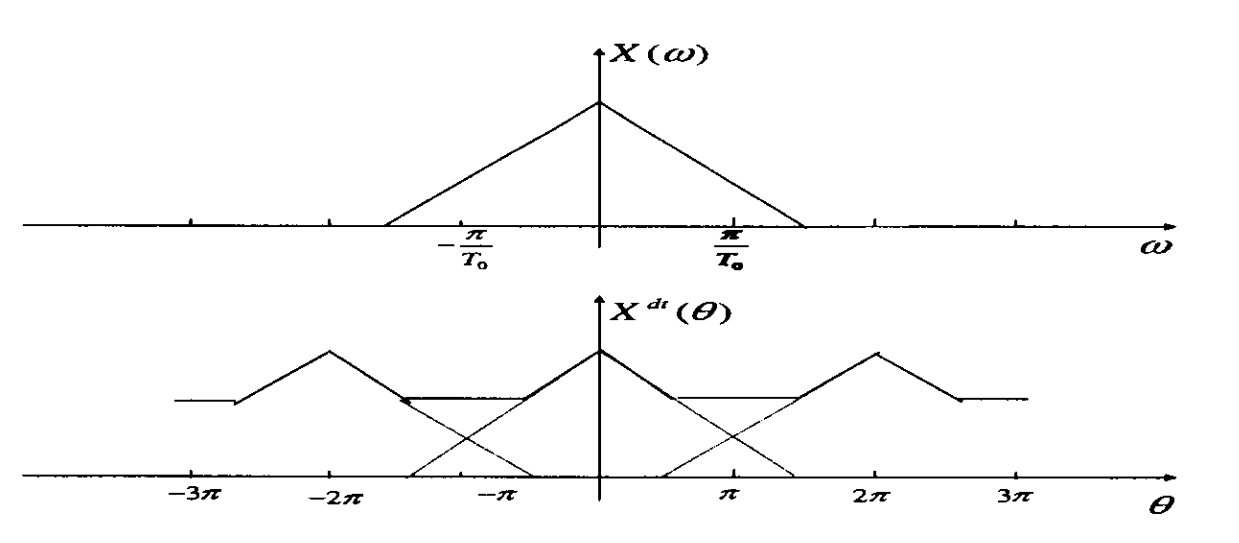
\includegraphics[scale = 1.0]{images/Aliases-under sampled.png}
        \caption{Original spectrum (top) and DTFT and overlapping replicas (bottom) \cite{SP_03_textbook}}
        \label{Aliases_underSamp}
\end{figure}
A corollary of \ref{Nyq-Shan} is that any signal with infinite bandwidth will always have overlapping spectrum replicas. Meaning, reconstruction of such a signal from it's samples is not possible.

% ======================================================
\section{Discrete Time System Classification}
In the simplest terms, a discrete-time system is a transformation, $\mathcal{T}\{\}$, which maps any given input sequence $x[n]$ to an output sequence $y[n]$. This output sequence may be referred to as the system response and is given below.
$$ y[n] = \mathcal{T}\{ x[1], x[2], ..., x[n], ... \} $$

\subsection{Linear Systems}
A linear system is any system under which both \textbf{superposition} properties are always true. These two properties are that of \textbf{scaling} and \textbf{additivity}. The scaling property states that, given an input $x[n]$ that produces an output $y[n]$ under transformation, the same input scaled by a constant will produce the same corresponding output scaled by the same constant. \vspace{-3mm}
\begin{align*}
&\mathcal{T}\{x[n]\} = y[n] \\
&\Longrightarrow \mathcal{T}\{ \lambda x[n]\} = \lambda y[n]
\end{align*}
The additivity property states that the addition of input sequences under transformation will result in the addition of the two corresponding output sequences.
$$\mathcal{T}\{x_1[n] + x_2[n]\} = y_1[n] + y_2[n]$$

\subsection{Time-invariant Systems}
A time-invariant system is one which, under the presence of translation at the input, will produce the same translation at the output.
\begin{align*}
&\mathcal{T}\{x[n]\} = y[n] \\
&\Longrightarrow \mathcal{T}\{ x[n-n_0]\} = y[n-n_0]
\end{align*}

\subsection{Causal Systems}
A causal system is any system for which any given output is not influenced by inputs from the future. An example of a non-causal system would be one such as $y[n_0] = x[n_0 + 1]$, for instance.

\subsection{Stable Systems}
A stable system is one which demonstrates, for a bounded input, a bounded output. This mathematical bound is analogous to limiting the amplitude of a signal, which is commonplace in any quantization process.
\begin{align*}
& |x[n]| \leq B_1 \leq \infty \\
&\Longrightarrow |y[n]| \leq B_2 \leq \infty
\end{align*}

% \subsection{The Linear, Time-Invariant Property}
% ON PAGE 42, INCLUDE IF NECESSARY OR CONVOLUTION IS BROUGHT UP LATER IN THE PAPER.

% ======================================================
\section{Discrete Fourier Transforms}
\subsection{Defining the DFT}
The Discrete Fourier Transform (DFT) is a computationally feasible version of the DTFT. It is obtained by sampling the DTFT in the frequency domain. For a signal with finite sequence length $N$, the DFT is given by definition \ref{DFT_def}.
\begin{align}\label{DFT_def}
    X^d[k]  &= \sum_{n=0}^{N-1}x[n]\exp{\Big( -\dfrac{j2\pi kn}{N} \Big)}, \hspace{3mm} 0\leq k \leq N-1
\end{align}
The key advantage of the DFT is that, by sampling the DTFT at $N$ points, we are able to reconstruct the original signal. The DTFT, on the other hand, required knowledge of the transform at infinitely many points. This is infeasible for a computing system and for this reason the DFT becomes very important. Similarly to the previously defined inverse Fourier transform, the inverse DFT is given in \ref{IDFT_def}.
\begin{align}\label{IDFT_def}
    x[n]  &= \dfrac{1}{N} \sum_{n=0}^{N-1}X^d[k]\exp{\Big( \dfrac{j2\pi kn}{N} \Big)}, \hspace{3mm} 0\leq n \leq N-1
\end{align}
\subsection{Disadvantages of the DFT}
It must be noted, whilst using the DFT, that there is an inherent limit in frequency resolution as opposed to previously mentioned methods. This is because, by analysing a signal of fixed duration $N$, we introduce gaps in between analysed frequencies of width $\Delta \theta = 2 \pi / N$. As is seen from this fraction, the gaps will decrease as the length of the signal increases, also increasing the frequency resolution. However, this poses a large issue for the analysis of short sequences as the resolution in the frequency domain will become severely limited. One such technique to work around this limitation is by using \textbf{zero-padding} to plaster the gaps of the DFT analysis. This will not be discussed in this paper. 

% ======================================================
\section{Short-Time Fourier Transforms}
\subsection{What Necessitates the STFT?}
Typical signal processing methods are performed on signals which are not time varying, and as a result do not change frequency over time. Speech signals, however, are much more complicated than this. As one would be familiar with, when vocalising a complex speech pattern the pitch of your voice may increase and decrease over time. Such is demonstrated in a natural speech signal, which can be characterised by shifting of the signals frequency peaks with respect to time. \\ \\
In such a scenario, an engineer may not want to apply a global transform to an input signal. Such a transform would be representative of those which this paper has concerned itself with up until this point. Instead, one may consider using a number of transforms over smaller intervals of the signal. It is this extension upon previous methods that forms the basis for the Short-Time Fourier Transform (STFT).

\subsection{Defining the STFT}
We may define a windowing function by $w(n-m)$. Such a function is usually symmetric about its midpoint $m=n$. This window function starts near or at zero, then increases to a maximum at the center of the time series and decreases again \cite{heinzel2002spectrum}. Common window functions include Hamming, Hanning and Rectangular windows. After this, the STFT can be defined by \ref{STFT_def}.
\begin{equation}\label{STFT_def}
    X[n, \theta]  = \sum_{m=-\infty}^{\infty} x[m]w[n-m]e^{-j\theta m}, \hspace{3mm} \theta \in \mathbb{R},n \in \mathbb{N}
\end{equation}

\subsection{Multi-Resolution via Spectrogram}
As a STFT is composed of different transforms over a time range, when we take the magnitude of the STFT we do not obtain the same result as for typical Fourier Transforms. Instead we obtain a plot with both a time dimension and a frequency dimension. This is known as a \textbf{spectrogram}. Typically this is plotted by using time as the x-axis, frequency as the y-axis, and colour to indicate the corresponding magnitude at a specific time and frequency. Many contemporary speech recognition and SER machine learning strategies will use some form of spectrogram as inputs, (among other things). They are incredibly useful for deciphering both speech and underlying emotions. One of these graphs, and its corresponding time series counterpart, is depicted in figure \ref{t_spec_plot}.
\begin{figure}
        \centering
        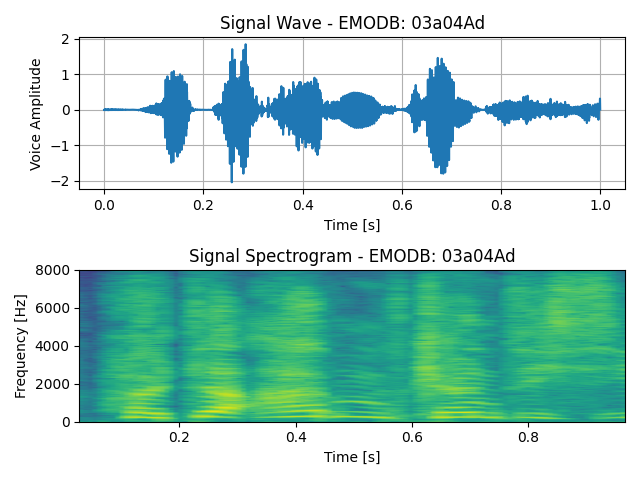
\includegraphics[scale = 0.8]{images/PLOT_TimeANDSpectrogram.png}
        \caption{Spectrogram of emotional speech}
        \label{t_spec_plot}
\end{figure}
It is of important note that the spectrogram does possess its flaws. The window bandwidth (frequency domain) and window time-frame (time domain) are identical under the Fourier transform. It follows that having both a small window bandwidth and small window time-frame, as to capture as much data as is attainable, is not possible. This means that any increase to the granularity of detail in one axis comes at a sacrifice to the detail in the alternate axis. 

% ======================================================
\section{Speech Signals}
Speech can be defined as any acoustic signal, typically created by a human, with frequency content existing within the human range of hearing. This range is approximately from $20Hz$ to $20kHz$. However, realistic ranges are often in between the lower and upper thresholds. As the signal composition of speech is very complicated, speech processing often involves extracting what the engineer deems to be the most useful information. Acoustic signals like speech have many characteristics and deciding which to isolate are application dependent. These extracted characteristics are known as features. As is the case for other domains of machine learning, these features form the basis for analysis and network training. 

\subsection{Speech Signal Analysis - Time \& Frequency Domains}
When analysing speech signals we have the choice to analyse them over a particular domain. That is, we can analyse them over the time domain, frequency domain, or both. Each of these different domains highlight different features and properties of the speech signals. Time and frequency representations of a speech signal taken from the EMODB dataset are illustrated in figure \ref{t_and_f_plot}. \\ \\
When visualising or analysing these signals in the time domain, the signal is referred to as a waveform. The key observable property of the speech in this state is the amplitude as a function of time. This directly relates to the volume or perceived loudness of such a signal. \\ \\
More observable in the frequency domain representation are frequency 'peaks'. These peaks correspond to where the majority of energy is stored in the signal, with respect to frequency. The highest peak would indicate that, across the signal, the most energy is present at or near that particular frequency.
\begin{figure}
        \centering
        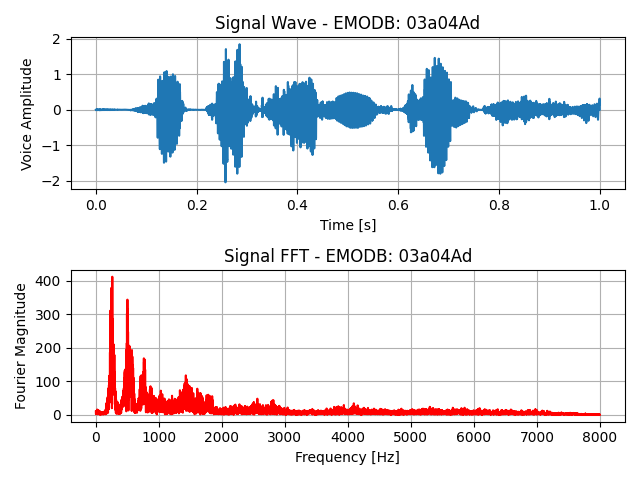
\includegraphics[scale = 0.8]{images/PLOT_timeAndFreq.png}
        \caption{Time and frequency representations of speech}
        \label{t_and_f_plot}
\end{figure}

\subsection{Fundamental Characteristics of Speech}
\begin{description}
\item[Overall Power:]
This is a measure for volume over the duration of the speech signal (or otherwise specified durations). Where amplitude is volume measured at an instant in time, overall power is essentially an average of volume over a range of time. This can give insights to the gender or emotional stress level of a speaker. 

\item[Short-time Power:]
Short-time power, as the name suggests, refers to the power observed over a shorter time frame. It is important to note that due to the linguistic complexity of speech production, speech signals are prone to changing drastically over very small time intervals. To capture this change, it is the role of a processing engineer to divide a signal into small windows of time. In doing so, the rapid and dynamic nature of the acoustic waveform should be roughly captured.\\ \\
Choosing a window length is application dependent due to the inherent trade-off of minimising window length. It would be ideal to have infinitely small time windows, as to capture every microscopic change in dynamic speech. However, this would result in enormous amount of digital processing, which is not computationally feasible. Thankfully, we can use insights from speech pathology to inform us of suitable window lengths which will not overburden a computer. The content of the speech signal can also drastically alter the required size of time windows. For example, long vowels  sounds can be captured with sufficient detail with time-frames of ~100 ms. However, other more abrupt noises may require windows of 5ms to 10 ms \cite{SP_03_textbook}. In general, the vocal tract system of a human deforms at a relatively slow rate. For this reason, the approximation can be made that speech signals do not vary over a window length of $\approx 10ms$ \cite{introtoDSP_core2}. The speech signal over these non-varying windows are referred t as \textit{stationary}.

\item[Fundamental Frequency:]
The fundamental frequency, $F_0$, is conventionally associated with the pitch of the speaker. In terms of SER, it is one of the most revealing features. It is crucial for identifying a subjects intonation; the rise and fall of one's pitch as they produce a speech signal. This intonation can be directly related to a current emotional state.

\item[Frequency Spectrum:]
This refers to the band of frequency of which the signal exists within. For example, if a human male was speaking between frequencies of $200Hz$ and $800Hz$ the spectrum would lie mostly between these two values. This range of frequencies is also known as the bandwidth of a speech signal. An example of the overall frequency spectrum is plotted in the bottom subplot of figure \ref{t_and_f_plot}.

% \item[Short-time average zero-crossing rate:]???

% \item[Short-time autocorrelation function:]???

\end{description}

% ======================================================
% \section{Tracking Speech and It's Formants}
% IN SECTION 2.4 OF TEXTBOOK


% ======================================================
\section{Fundamental Frequency Calculation}
Due to the non-stationary nature of speech (dynamically time-variant), among other factors, the calculation of $F_0$ is rather complex. It is also one of the most formative features of speech signals. Thus, their is a large importance placed upon accurate calculation of the fundamental frequency. 
\\ \\
Speech can, however, be approximated as periodic and stationary over a small enough timescale. As the signal is quasi-periodic, it follows that the fundamental frequency will generate additional harmonics at integer multiples of $F_0$. If one works backwards from the frequency spectrum, by observing the placement of the harmonics one may be able to estimate the fundamental frequency. $F_0$ Can also be calculated through time domain methods, however, this typically yields a lower accuracy \cite{SP_03_textbook}. It does typically provide a means of more efficient computation though. The basic process of estimating pitch is summarised by the subsequent steps.
\begin{itemize}
    \item \textbf{Pre-processing:} This typically involves some kind of filtering or adjustments made to the signal. Such adjustments are made to create a simplified signal which is easier to process.
    
    \item \textbf{Extraction:} This refers to the actual estimation of $F_0$ for the specific signal being analysed at that time. The quantity can be derived from the perspective of the time or frequency domain. 
    
    \item \textbf{Post-processing:} Given that the fundamental frequency obtained is an estimate, this process is prone to errors. This final step involves forms of error correction. This can look like enforcing continuity over the set of calculated frequencies for all windows.
\end{itemize}

% \subsection{Time Domain Calculation}
% \subsection{Frequency Domain Calculation}



% ======================================================
\section{Phonetic Classification of Speech}
While a mathematical classification of speech and its fundamentals is incredibly useful for DSP applications, a phonetic classification is also necessary. Through understanding the physical processes used in the creation of speech, one may better design DSP systems. Notably, this understanding is vital for feature identification.
\\ \\
Speech can be classified as a pressure based waveform, traditionally created by a human. Most people relate speech waveforms to a signal emitted from one's mouth. While this is correct, the signals are created by complicated processes also involving the vocal tract, nostrils, and other body parts. All of these body parts will vibrate in specific ways, creating sound. Among the main tools shaping the speech output are the vocal tract and vocal cords. They are responsible for volume and pitch of the emitted signal. These sounds can be analysed on a 'chunk by chunk' basis. The resulting fragmented speech chunks are referred to as \textbf{phones}. The most fundamental unit of speech is a \textbf{phoneme}. These are essentially distinct sounds, used to differentiate words and larger units of speech from one another. Phones are the acoustic, audible counterparts of phonemes. In order to create a particular phoneme verbally, one must correctly position their jaw, teeth, tongue, velum, lips and their vocal cords. It is simple to see, upon further inspection, how complicated the speech generation process is mechanically, via the necessary collaboration of so many articulatory systems. Phonemes can generally be classed as one of two categories in speech processing. The first category of phonemes is vowels. These typically manifest as more intense sounds. The second category is consonants. These phonemes impose a constriction on the vocal tract and limit the airflow through it. On the contrary, vowels impose no limit on vocal tract airflow.




%=======================================
%	Chapter 3
%=======================================
\chapter{Literature Review - Speech Classification}\label{ch-lit-rev}
Having reviewed the acquisition and processing of speech-like signals, this text now seeks to define emotion from a speech signal context. While a number of features can be used to indicate an emotion present in a speech signal, (refer to table \ref{Emo_Char_Tab}), the CyTex transform is primarily (and almost solely) interested in pitch. However, it must be noted that classification is conducted on the basis of a deep learning framework. This means that manual feature extraction is not necessary. Although, the CyTex is a means of implicitly extracting certain features from an audio file. Different models of emotion are defined for reference within this chapter. This section also introduces the reader to SER from a high level, detailing each step of the process. Contemporary methods and models tested on well known SER datasets are briefly detailed. These modern studies function as comparative points to grade the success of CyTex relative to established approaches. Their implementation and results are primarily discussed. Finally, a number of the challenges facing current researchers are presented, some of which CyTex addresses.


% SECTION:
% ================================================
\section{Defining Emotion in Speech Signals}
Interestingly, no consensus definition of emotion exists in the psychological research community \cite{surveyCORE1}. Part of the reason may be the many ways to classify a concept as broad as emotion. By constraining the definition of emotion to one within the domain of speech, this definition becomes easier to construct, although less rigorous. However, the rigour used is sufficient for machine learning applications. Two models of emotion are considered, with varying simplicity and robustness. These models are the \textbf{discrete emotional model} and the \textbf{dimensional emotional model}.
\subsection{The Discrete Emotional Model}
Six prominent categories of emotions have been formulated as the "building blocks" of other emotions. These emotions consist of sadness, happiness, fear, anger, disgust and surprise, as suggested by \cite{ekman2013emotion}. In defining these as \textit{basic emotions}, it is implied that more complicated emotions are expressed as combinations of the basic emotions. While this model is simple and easy to interpret, some researchers believe it lacks the ability to clearly express more complicated emotions. This emotional model (or one tangential to it) is often used in the construction of emotional speech datasets like the EMODB dataset \cite{EMODB_97}. It allows for simple labelling of data and identification of the target classification. 

\subsection{The Dimensional Emotional Model}
This model of emotional state was developed to describe all emotional states \cite{RUSSELL1977}. This model opts for com[posing emotion of broad factors/dimensions. In particular, these include valence, arousal, control and power. In defining all emotions in terms of these dimensions, as opposed to separate base emotions, we can better define what makes an emotion. \cite{nicolaou2011} notes that most emotions can be characterised by two dimensions: valence and arousal. \textit{Valence} describes the positivity of an emotion, described in terms of pleasant or unpleasant. \textit{Arousal} details the relative strength of a particular emotion to the subject exhibiting that emotion. For example, anger would have a large arousal strength, where as an emotion like boredom would typically have a much smaller arousal strength. The use of arousal and valence as the defining criteria for emotional states is a popular two-dimensional model. Dominance/power may be included as a third dimensional to give a more robust model of emotion and further differentiate between emotions. This characteristic is effectively the perceived strength of a subject displaying an emotional reaction. Depending on the number of dimensions used, however, some emotions may appear as identical. One may obviously note that a large number of dimensions may be required to sufficiently describe all emotions. This is infeasible in a machine learning setting and as such there is an inherent trade off between dimensions and precision. Also, unlike the discrete emotional model, classification of emotions loses its ease of identification. 

\subsection{Prosodic Features of Emotional Speech}
Many SER systems utilise prosodic features for the classification of emotion in acoustic signals. These features are intuitive for humans as they form the basis for verbal communication. All verbal speakers are familiar with features like pitch, intensity and speaking rate. A sufficient summary of prosodic features is detailed in table \ref{Emo_Char_Tab} and related to corresponding emotions that exhibit such features, (excerpted from \cite{Ramakrishnan12}). Contemporary literature has previously demonstrated a preference for the use of prosodic features, as they yield more distinct properties than their non-prosodic counterparts. In particular, \cite{zeng2009} notes that a large amount of research in this field points to pitch (fundamental frequency) and energy forming the largest basis for recognising emotion.
\begin{table}[h]
% [h] argument will place the table here approximately.
% centering not working so use negative hspace instead!
    % \centering
    \hspace*{-2.5cm}
    \begin{tabular}{|l||p{2cm}|p{2cm}|p{2cm}|p{2cm}|p{2cm}|}\hline
        \backslashbox[14em]{\textbf{Characteristics}}{\textbf{Emotions}}
        & \textbf{JOY} & \textbf{ANGER} & \textbf{SADNESS} & \textbf{FEAR} & \textbf{DISGUST}\\\hline\hline
        Pitch Mean &High &Very High &Very Low &Very High &Very Low\\\hline
        Pitch Range &High &High &Low &High &High-male, Low-female\\\hline
        Pitch Variance &High &Very High &Low &Very High &Low\\\hline
        Pitch Contour &Incline &Decline &Decline &Incline &Decline\\\hline
        Intensity Mean &High &Very High-male, High-female& Low& Med/High &Low\\\hline
        Intensity Range &High &High &Low &High &Low\\\hline
        Speaking Rate & High & Low-male, High-female & High-male, Low-female & High & Very low-male, Low-female\\\hline
        Transmission Durability &Low &Low &High &Low &High\\\hline
        Voice Quality &Modal/tense &Breathy; med blaring timbre &Resonant timbre &Falsetto &Resonant timbre\\\hline
    \end{tabular}
    \caption{Emotional Acoustic Characteristics \cite{Ramakrishnan12}}
    \label{Emo_Char_Tab}
\end{table}


% SECTION:
% ================================================
\section{Speech Emotion Recognition - An Overview}
SER encompasses the methods and techniques employed to detect emotion(s) within speech signals. The core inclusion of an SER system is some supervised learning model which seeks to classify these emotions. Figure \ref{ser_branch_fig} illustrates a broad view of some of the major considerations of building an SER system. Generally, in working through an SER related task, one would traverse from left to right in this diagram. While not every sub-branch is necessary for successful implementation, each should be considered.
\begin{figure}[h]
        \hspace{-1cm}
        % \centering
        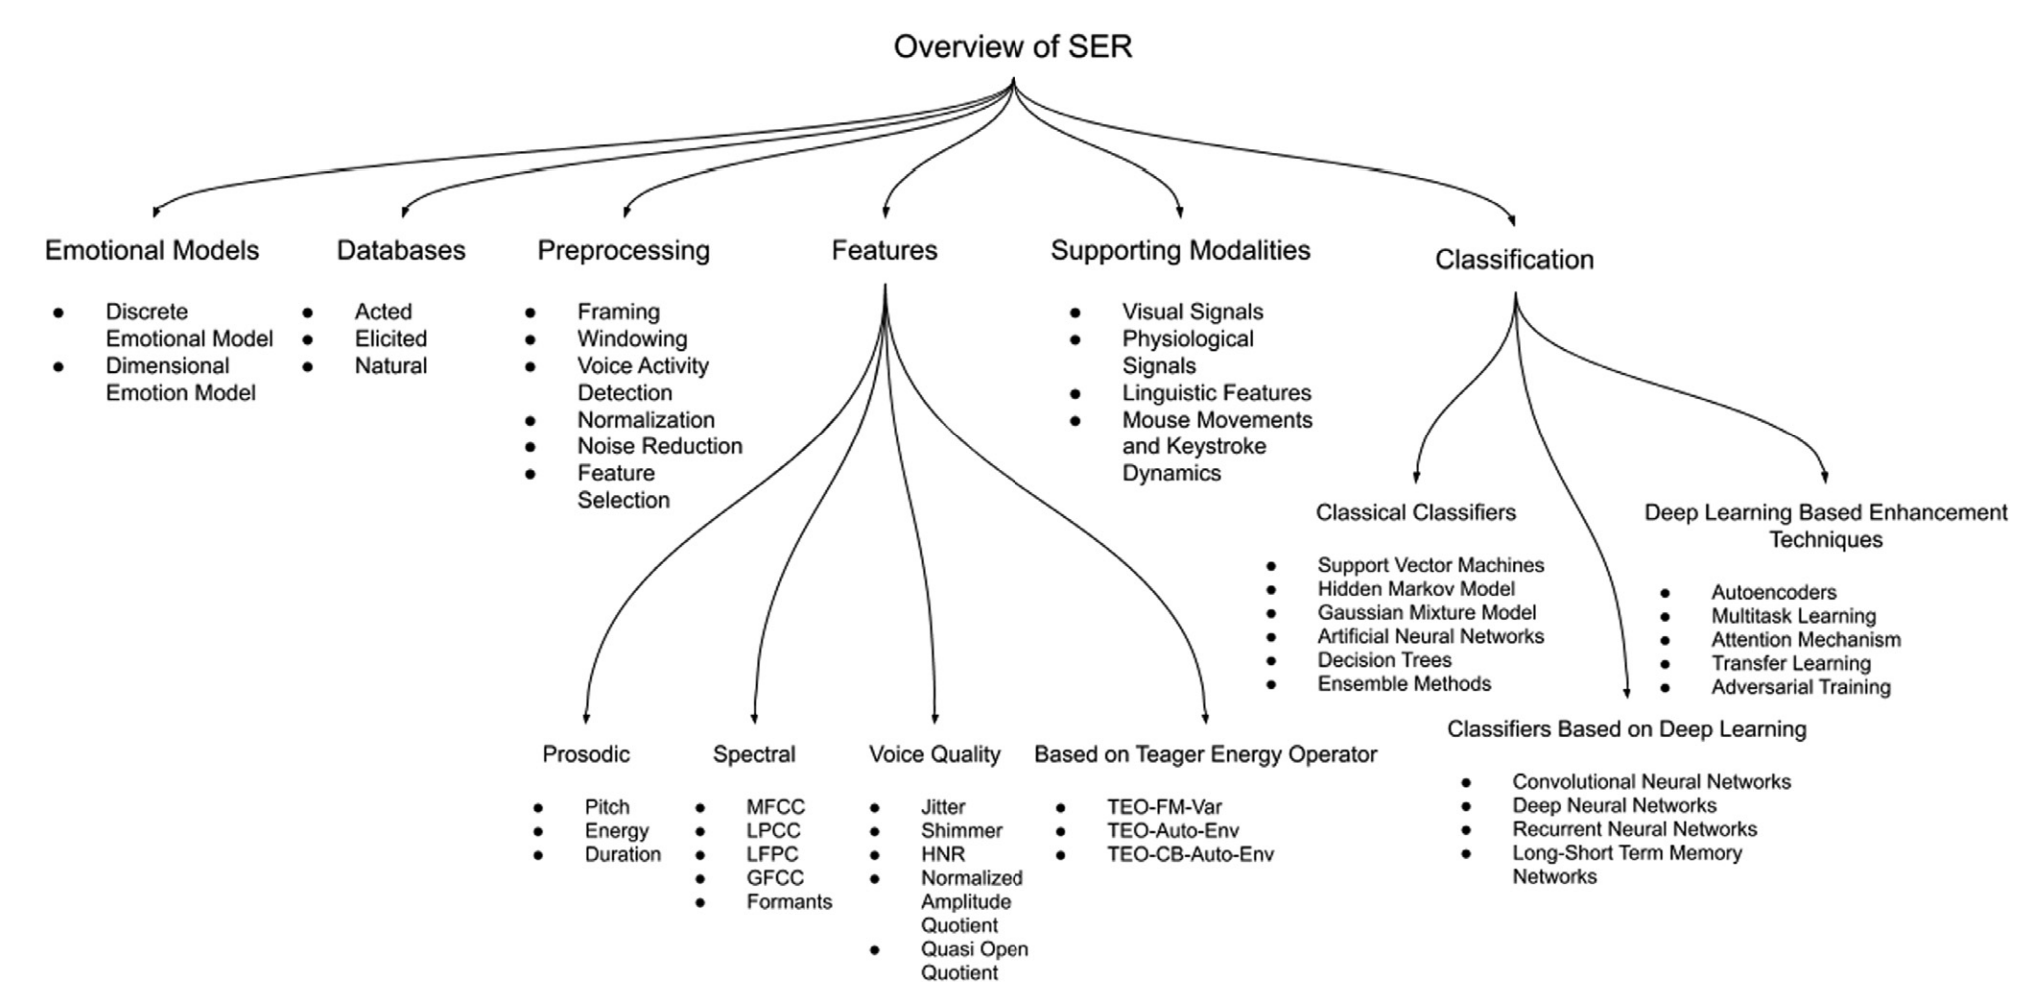
\includegraphics[scale = 1.0]{images/SER Overview Map.png}
        \caption{SER Overview \cite{surveyCORE1}}
        \label{ser_branch_fig}
\end{figure}
 Different models for emotion have been discussed in detail in the sections prior and the databases of SER are detailed in chapter \ref{ch-theory}. The CyTex transform itself serves as a means of employing preprocessing and preliminary feature extraction, also discussed in chapter \ref{ch-theory}. Supporting modalities are other media which support a classifier in determining which emotion is present in a data sample. This may involve things like video and facial motion capture. However, this study is solely interested in the analysis of acoustic audio data. As such, supporting modalities will not be addressed within this thesis. A number of classification schemes can be utilised in SER, including traditional machine learning approaches or advanced deep learning approaches. This study employs a deep learning approach based on a convolutional neural network architecture and utilises transfer learning for model enhancement. Both of these topics are discussed in further detail in chapter \ref{ch-theory}.\\ \\
 Figure \ref{ser_pipeline_fig} details a similar, albeit simplified, framework for the implementation of an SER system. Here the signal source will be some acoustic signal from a labelled emotional audio dataset. Feature extraction synthesises key identifiers of emotional from the signal source. Post processing is used to 'clean' the format of the incoming signal prior to selecting which features to use for training and classification. Following this, a machine learning model is trained and employed as a means of classifying data. It should be noted that a more common approach is to implement some form of preprocessing initially and then perform feature extraction and selection in a single step. When using a deep learning model as a classifier, feature extraction and selection can be discounted entirely.
\begin{figure}[h]
        \centering
        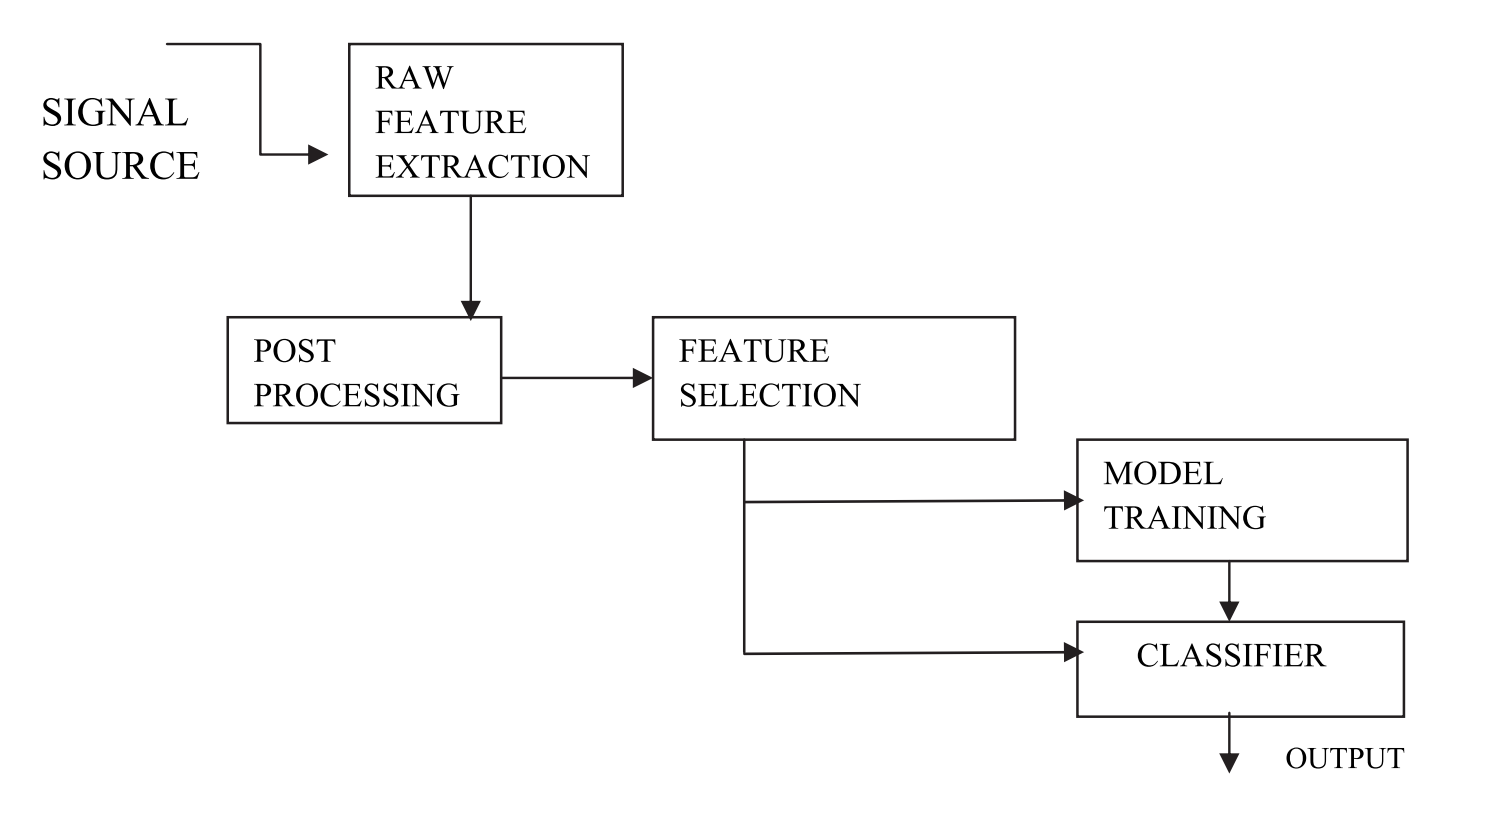
\includegraphics[scale = 1.0]{images/Basic SER framework.png}
        \caption{Basic SER Framework \cite{Ramakrishnan12}}
        \label{ser_pipeline_fig}
\end{figure}

\subsection{SER Using Deep Learning}
In this study a deep learning algorithm is used to classify the emotion of acoustic signals. This deep learning algorithm is trained on CyTex images, defined in chapter \ref{ch-theory}. While the CyTex images perform some kind of feature extraction, these features are not explicitly provided to the deep learning model. With advancements in technology and its access, the popularity of deep learning has increased. This increase in the application of deep learning usage has also seen improvements in results on benchmark SER datasets. As noted previously, deep learning possesses the benefit of requiring no manual extraction or selection of features from the data. The deep learning model will automatically 'learn' which features provide the best means of classification.


% SECTION:
% ================================================
\section{Benchmarks \& Contemporary Methods}
The two key datasets that this dissertation aims to focus on are the EMODB and RAVDESS datasets. To give a fair point of comparison for the developed model's performance other benchmark methods have been studied for the same datasets. Methods highlighted employ novel schemes and have achieved high accuracy on their respective datasets. Not all methods utilised in contemporary studies will be rigorously define. Readers are encouraged to to access the provided reference papers of contemporary methods for more comprehensive explanations on applied procedures. This section merely highlights general strategies and the prominent results of each case.

\subsection{Stacked Autoencoder Network \& Deep Belief Network}
Two models are constructed by Zhou et al. harnessing a Stacked Autoencoder (SAE) network and a Deep Belief Network (DBN) \cite{zhou2016deep}. In using deep learning, emotional feature extraction is automated, reducing complexity of implementation and eliminating subjectivity of feature selection. Audio files from the EMODB dataset are used as direct inputs into the model. Preprocessing begins with signal sampling at $16kHz$. This is followed by dividing the data into $50ms$ frames (to be considered stationary) via Hamming windowing. Each Hamming window has a length of 256 and contains an overlap percentage of $50\%$. Following this the frames are divided into a training and test set and fed into the deep learning model. This process is depicted in figure \ref{zhou2016_flowchart}.\\ \\
\begin{figure}[h]
        \centering
        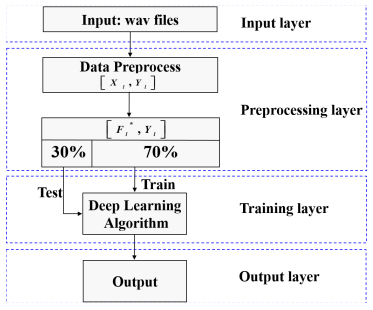
\includegraphics[scale = 0.8]{images/zhou_flowchart_fig.png}
        \caption{SER via Direct Signal Learning \cite{zhou2016deep}}
        \label{zhou2016_flowchart}
\end{figure}
In the SAE approach, autoencoders are placed in a sequential pipeline. Following this, parameters are fine tuned and autoencoders are stacked in a network. The DBN is based on a Restricted Boltzmann Machine (RBM). RBM's are trained and also pipelined. After stacking these machines and retraining several times, one obtains a DBN.\\ \\
During testing on the EMODB dataset, recognition accuracy reached a height of $65.00\%$ for both models (although the stacked autoencoder approach was marginally lower). However, in this case the number of predicted emotional states was reduced to two. Both models demonstrated significantly worse performance when required to predict seven emotional states. The SAE model exhibited an accuracy of $25\%$, while the DBN demonstrated an accuracy of $38\%$. While this accuracy is significantly lower than the other methods discussed in this paper, it is still important. This result contextualises the performance of deep learning when applied directly to audio signals. Such results also suggest that both methods of feature extraction do not yield salient enough features for the basis of classification.

\subsection{Deep 1D \& 2D CNN-LSTM Networks}
Zhao et al. employs two different CNNs and LSTMs and compares the two systems. The first of the two CNNs (1D) aims to model local emotional features extracted from the speech signal itself. The second CNN (2D) analyses log-mel spectrogram images to learn features that more globally describe the emotional content of a signal \cite{ZHAO2019}. Models share closely related architectures containing four local feature learning blocks (LFLBs). Each of these blocks are composed of a convolutional layer, batch normalization layer, exponential linear unit layer and finally a max-pooling layer. These blocks are proceeded by a single LSTM layer in each case. The LSTM layers specialise in learning long-term dependencies, which in the case of log-mel spectrogram approaches, is traditionally lacking. This counteracts the frequency/time trade-off of log-mel spectrogram generation to some degree. Figure \ref{zhao2019_arch_fig} illustrates a block diagram comprised of the discussed blocks.\\ \\
\begin{figure}[h]
        \centering
        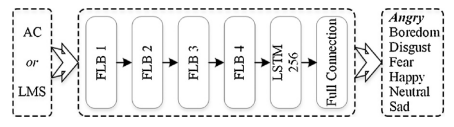
\includegraphics[scale = 1.0]{images/zhao_architecture.png}
        \caption{1D and 2D CNN-LSTM Architectures \cite{ZHAO2019}}
        \label{zhao2019_arch_fig}
\end{figure}
The training and validation results of the two-dimensional CNN-LSTM architecture are displayed in figure \ref{zhao2019_train_fig}. The largest validation accuracy achieved for the EMODB dataset was $76.64\%$. After validating and testing the data on the EMODB dataset, an average accuracy of $95.33\%$ was achieved through use of the two-dimensional model. The one-dimensional model performed less favourably, achieving an average accuracy of $86.73\%$. These metrics were found by retrieving the confusion matrix of classification rates across all emotion types and averaging the correct prediction percentages for each. This result is one of the highest benchmarks on this dataset in recent years. Exemplary results were also demonstrated on the IEMOCAP database. An accuracy of $89.16\%$ was achieved utilising the same two-dimensional CNN-LSTM approach. 
\begin{figure}[h]
        \centering
        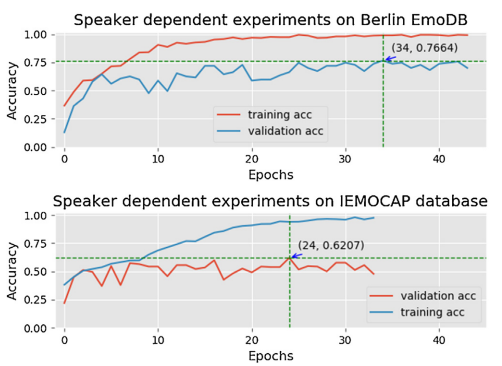
\includegraphics[scale = 0.8]{images/Zhao-2dCNN_trainvalResults.png}
        \caption{2D CNN LSTM train-val Accuracy \cite{ZHAO2019}}
        \label{zhao2019_train_fig}
\end{figure}

\subsection{3D CNN for Spectro-Temporal Feature Learning}
The addition of LSTM blocks to the output of CNN systems introduces increased model complexity. In attempts to capture important temporal data, without the addition of LSTM blocks, Kim et al. presents an additional dimension in a CNN architecture \cite{kim2017speech}. These three-dimensional CNN structures are capable of simultaneous short and long-term spectral feature extraction. Such models were found to be more effective than other methods in the domain of spectro-temporal feature extraction and classification. Figure \ref{3dcnn_fig} depicts a two-dimensional CNN which is fed into LSTM layers (a), and a three-dimensional CNN. In (a), a 2D convolution is applied to each spectral image (feature map). These spectral feature maps are arranged in time (annotated L). By applying a 3D convolution to a time series of feature maps, we preserve the three-dimensional structure of the input. \\ \\
\begin{figure}[h]
        \centering
        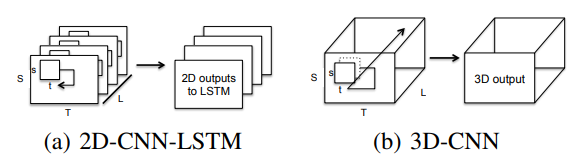
\includegraphics[scale = 0.8]{images/3dcnn_IMG.png}
        \caption{Differing Dimensions of CNN Architectures \cite{kim2017speech}}
        \label{3dcnn_fig}
\end{figure}
The dataset used for the training and validation of this approach was created by aggregating seven other SER datasets. Thus, the specific accuracy metrics are not provided for the EMODB, RAVDESS or IEMOCAP datasets. This approach did, however, outperform a number of \textit{'off the shelf'} methods on the constructed dataset, like those proposed in \cite{ZHAO2019}.


% Check definition of speaker independent???
% \subsection{A Speaker Independent SVM Approach}
% \cite{Shirani2016}

\subsection{Novel Temporal Emotional Modeling - TIM\_NET}
Temporal-aware bI-direction Multi-scale Network (TIM-Net) details a network capable of temporal learning on different time scales. Information from both the past and future instances of a signal are used to enhance feature representation \cite{ye2023temporal}. This appraoch seeks to remedy some common drawbacks of LSTM implementation. Specifically, an inability to capture long-term dependencies which inform context. Mel-Frequency Cepstral Coefficients (MFCCs) were chosen as inputs for the model. Framing and windowing is applied to inputs, utilising a Hamming window. The first 39 coefficients are utilised after further processing. The key method exploited in this system is the use of temporal-aware blocks which, in parallel, process forwards and backwards time cases of the input. These blocks analyse a number of consecutive frames and select the most affective. A causal constraint is applied to ensure the elimination of leakage from future to past samples. Feature outputs from the forward and backward direction paths are fused dynamically using weighted summation. The net process is represented in figure \ref{timnet_fig}, also further detailing the temporal-aware blocks.\\ \\
\begin{figure}[ht]
        % \hspace{-2.5cm}
        \centering
        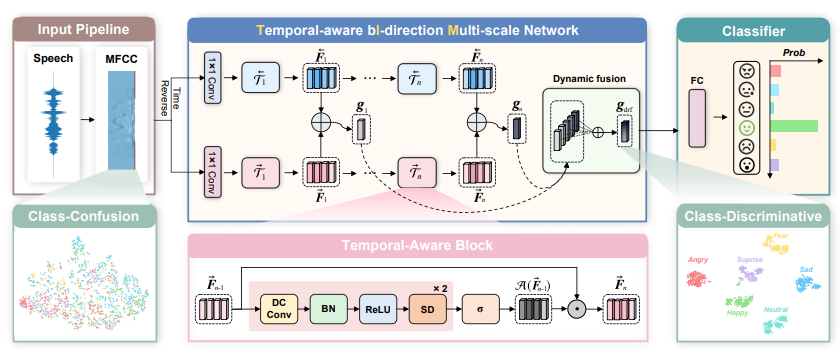
\includegraphics[scale = 0.8]{images/TIM_NET_fig.png}
        \caption{TIM-Net Framework for SER \cite{ye2023temporal}}
        \label{timnet_fig}
\end{figure}
TIM-Net has demonstrated exceptional results over a number of standard datasets within the SER community. Of interest for comparison to this study and those previously mentioned, the EMODB, RAVDESS and IEMOCAP databases are all utilised. Accuracy is measured using both Unweighted Average Recall (UAR) and Weighted Average Recall (WAR). The WAR measures seek to compensate for the imbalance of classes in some datasets. However, only the UAR results are noted here as they are directly comparable to the average accuracy specified in other contemporary methods. For the EMODB dataset, a UAR score of $95.17\%$ was achieved, existing in the same neighbourhood as other state of the art solutions. TIM-Net is one of the highest performing models on the RAVDESS dataset, demonstrating an average accuracy of $91.93\%$. Finally, this model achieved a $72.5\%$ UAR score on the IEMOCAP database. 


% \subsection{CNN-Assisted Enhanced Audio Signal Processing}
% \cite{kwon2020_cnn-assist}

% SECTION:
% ================================================
\section{Speech Processing Challenges}
Speech emotion recognition is still juvenile in the context of machine learning fields. This entails periods of rapid advancement, but comes with the disadvantages of numerous obstacles that the field is yet to overcome. Some of these are discussed subsequently and are recommended as further areas of research into the future of the SER field.

\subsection{Databases}
Any machine learning system is only as good as the data it is trained on. However, it is very difficult to approximate life-like emotional speech datasets for reasons discussed in chapter \ref{ch-theory}. Many of these reasons involve the legality of capturing real emotional responses. Those datasets that attempt to create more realistic emotional responses are often incomplete (emotionally) and are difficult to label. Annotation, in these circumstances, may introduce error into the dataset as the recognition rate is at or below $90\%$ \cite{surveyCORE1}.\\ \\
The validation of a model's performance is also dependant on its underlying database. Comparison between the performance of different models can prove difficult as models may be specialised for particular databases, or trained on separate ones altogether. \cite{zeng2009} notes the requirement of research communities unionising to formulate common evaluation procedures on comparative datasets. This will better allow for comparison of models and indicate their relative proficiency. 

\subsection{Cultural Barriers}
A universal SER model seems like an impossibility. A number of studies, attempt to recognise emotion for different languages. However, these methods typically exhibit lower accuracy than speaker dependent methods. The obvious caveat to methods that use prosodic features, for instance, is tonal languages. In non-tonal languages, features like pitch provide formative grounds for the classification of emotions. Whereas a tonal language utilises pitch to imply the meaning of speech, rather than the emotional state.

\subsection{Multi-Speech Recognition}
Further work should be conducted in the domain of identifying which signal, in a composition, a machine should focus on. In a real-world setting, it is likely that environments will be noisy and contain numerous acoustic signals. Algorithms that separate speech from ambient noise or other speech singals can be implemented in preprocessing, however, \textit{"current systems fail to notice this problem"} \cite{surveyCORE1}.
 
\subsection{Pre-trained Model Limitations}
Finally, that which CyTex and other image processing based approaches addresses, is the lack of pre-trained models able to be utilised for speech emotion recognition. This introduces a barrier into the field of SER as many methodologies require the construction and training of entirely new models. By converting audio signals to an image domain, a wealth of pre-trained and openly accessible deep learning models may be used.



% ===========================================
%	Chapter 4
% ===========================================
\chapter{Theory and Principles - Classification with CyTex}\label{ch-theory}
% SECTION:
% ================================================
\section{Fundamental Concepts of the CyTex Image}
Figure \ref{cytexFlowchart} details the stepped process of transforming a speech signal into an equivalent CyTex image. Such a process is likely necessary to learn insights of the time-frequency correlations of speech, suggested by \cite{zhang2017speech}.The two dimensional textured images are able to capture more information than a corresponding one dimensional audio signal. The following sections provide an in-depth reference of each of the function blocks present in figure \ref{cytexFlowchart}. 
\begin{figure}
        \centering
        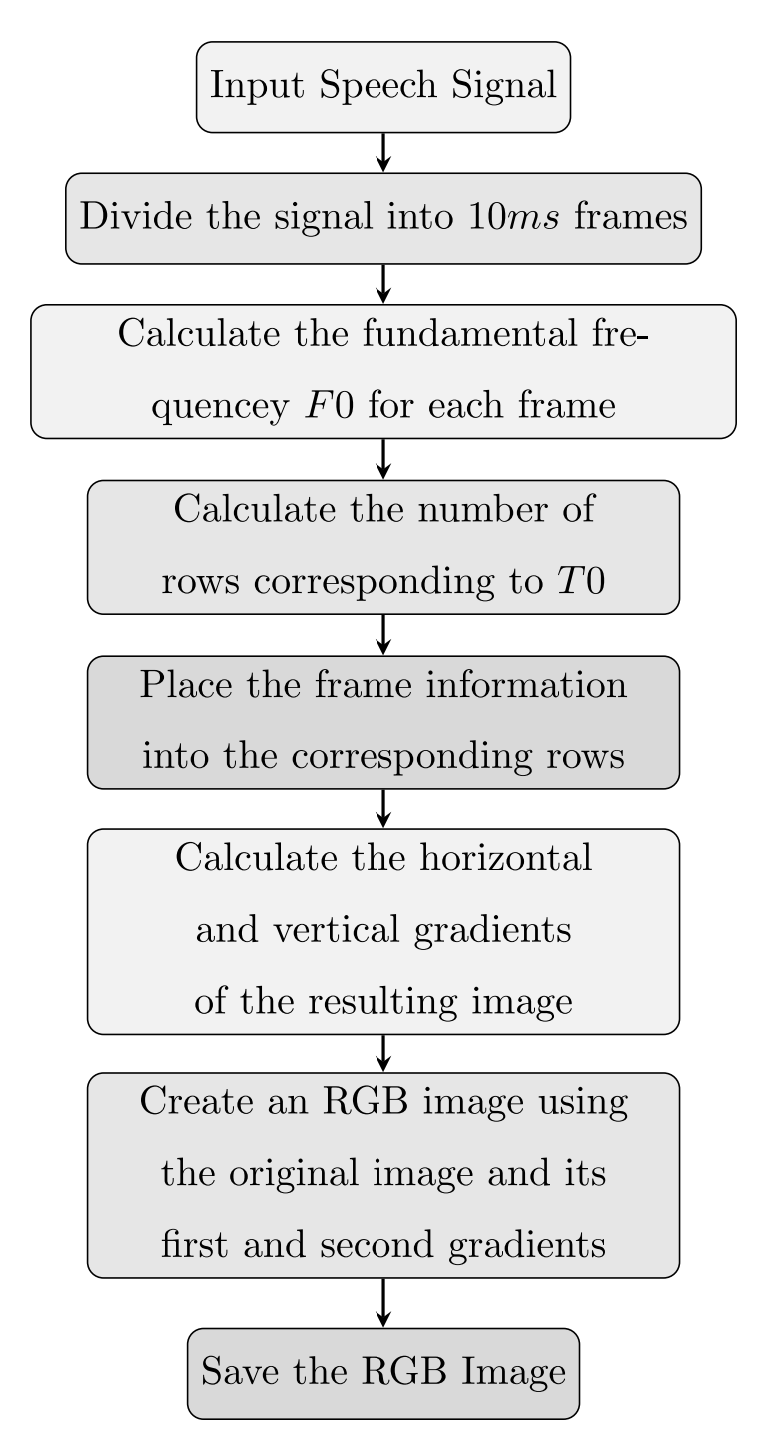
\includegraphics[scale = 0.8]{images/CyTex Procedure Flowchart.png}
        \caption{CyTex transformation process \cite{CyTexRef}}
        \label{cytexFlowchart}
\end{figure}
\subsection{Frame Division}
As speech signals are quasi-periodic, the demonstrate some periodicity, however, also vary in accordance with time. This means that analysing the signal on a global scale is a poor decision as at two distant time-points the signal will likely be drastically different. By dividing the audio signal into smaller width time-frames, as discussed when dealing with the STFT, one is able to capture the temporal evolution of the signal. Smaller time windows also better capture the intonation of speech. This information proves vital for the classification of emotions in this context. As was previously noted, a suitable window length of $10ms$ is chosen for most applications. This strikes a balance of being wide enough to minimise the processing required, while also being small enough to consider the signal as stationary over the time interval. Stationary refers to non-changing frequency and spectral contents over some time interval.

\subsection{Fundamental Frequency via Fourier Transform}
For each window frame $F_{0_n}$ is calculated using the librosa package \cite{mcfee2015librosa}. This uses a modified STFT approach to find the fundamental frequency. Specifications for duration and pitch thresholds must be declared by the user. It may be of interest to make these parameters dynamic or alterable when generalising CyTex to other kinds of data. As one can imagine, the pitch limits set are entirely dependent on the frequency production range of the type of acoustic data being analysed. For human speech contexts, limits of below $1kHz$ are a suitable choice. It is of very important note that the calculation of $F_{0_n}$ is extremely crucial. The benefit of CyTex is that the transform can be conducted purely on the knowledge of $F_{0_n}$. However, the disadvantage of this is that if such a calculation possesses significant error, the entire classification process will dramatically suffer. 

\subsection{Mapping to the Image Domain}
For each frame a fundamental frequency, $F_{0_n}$ is found. The inversion of this is the fundamental period $T_{0_n}$. Each of these periods are to a horizontal row of the CyTex image, having a vertical width of one pixel. This means that the $n^{th}$ row of the image will correspond to the $n^{th}$ fundamental period. The length of an image row is determined by the sampling rate and the minimum frequency allowance specified to the librosa package. The maximum length is provided in equation \ref{max_width_cytex}.  A sampling frequency, $f_s = 16kHz$, is chosen. This is because all humans should speak well within the band of $[0, 8kHz]$ and the upper limit is double to satisfy the Nyquist rate. Zero-padding is applied in cases where the pixel width does not take up the max length. In practical cases the lower frequency limit is set to $40Hz$ and thus the resulting length is $400$ pixels wide.
\begin{align}\label{max_width_cytex}
    S_{T_{max}} &= \dfrac{f_s}{f_{min}} \\ \nonumber
                &= \dfrac{16kHz}{40} \\ \nonumber
                &= 400
\end{align}
 The number of vertical rows is calculated as follows. This height is directly related to the duration of the entire the signal. So, the longer a signal is in the time scale, the taller the resulting CyTex image. 
\begin{align}\label{vert_rows_eqn}
    n = ceil \Big( \dfrac{160 F_{0_n}}{N_{F_{0_n}}} \Big)
\end{align}
Finally, the intensity of the pixels are directly related to the intensity of the signal at that specific point in time. The numerical range of values the pixels can take on is in between 0 and 255 due to the RGB nature of the output image. Pixel intensities at the upper or lower boundaries relate to more intensely felt emotions such as anger or immense joy. The intensity calculation is provided by equation \ref{P_intensity}. Here $S_n$ refers to the speech sampled value at a particular time instant.
\begin{align}\label{P_intensity}
    P_n = round \Big( \dfrac{255 (S_n + 1)}{2} \Big)
\end{align}
A detailed speech to image mapping is illustrated in figure \ref{cytexVis_example}. By working up from the base of the image one can see how a time series signal is mapped to the RGB image domain. 
\begin{figure}
        \centering
        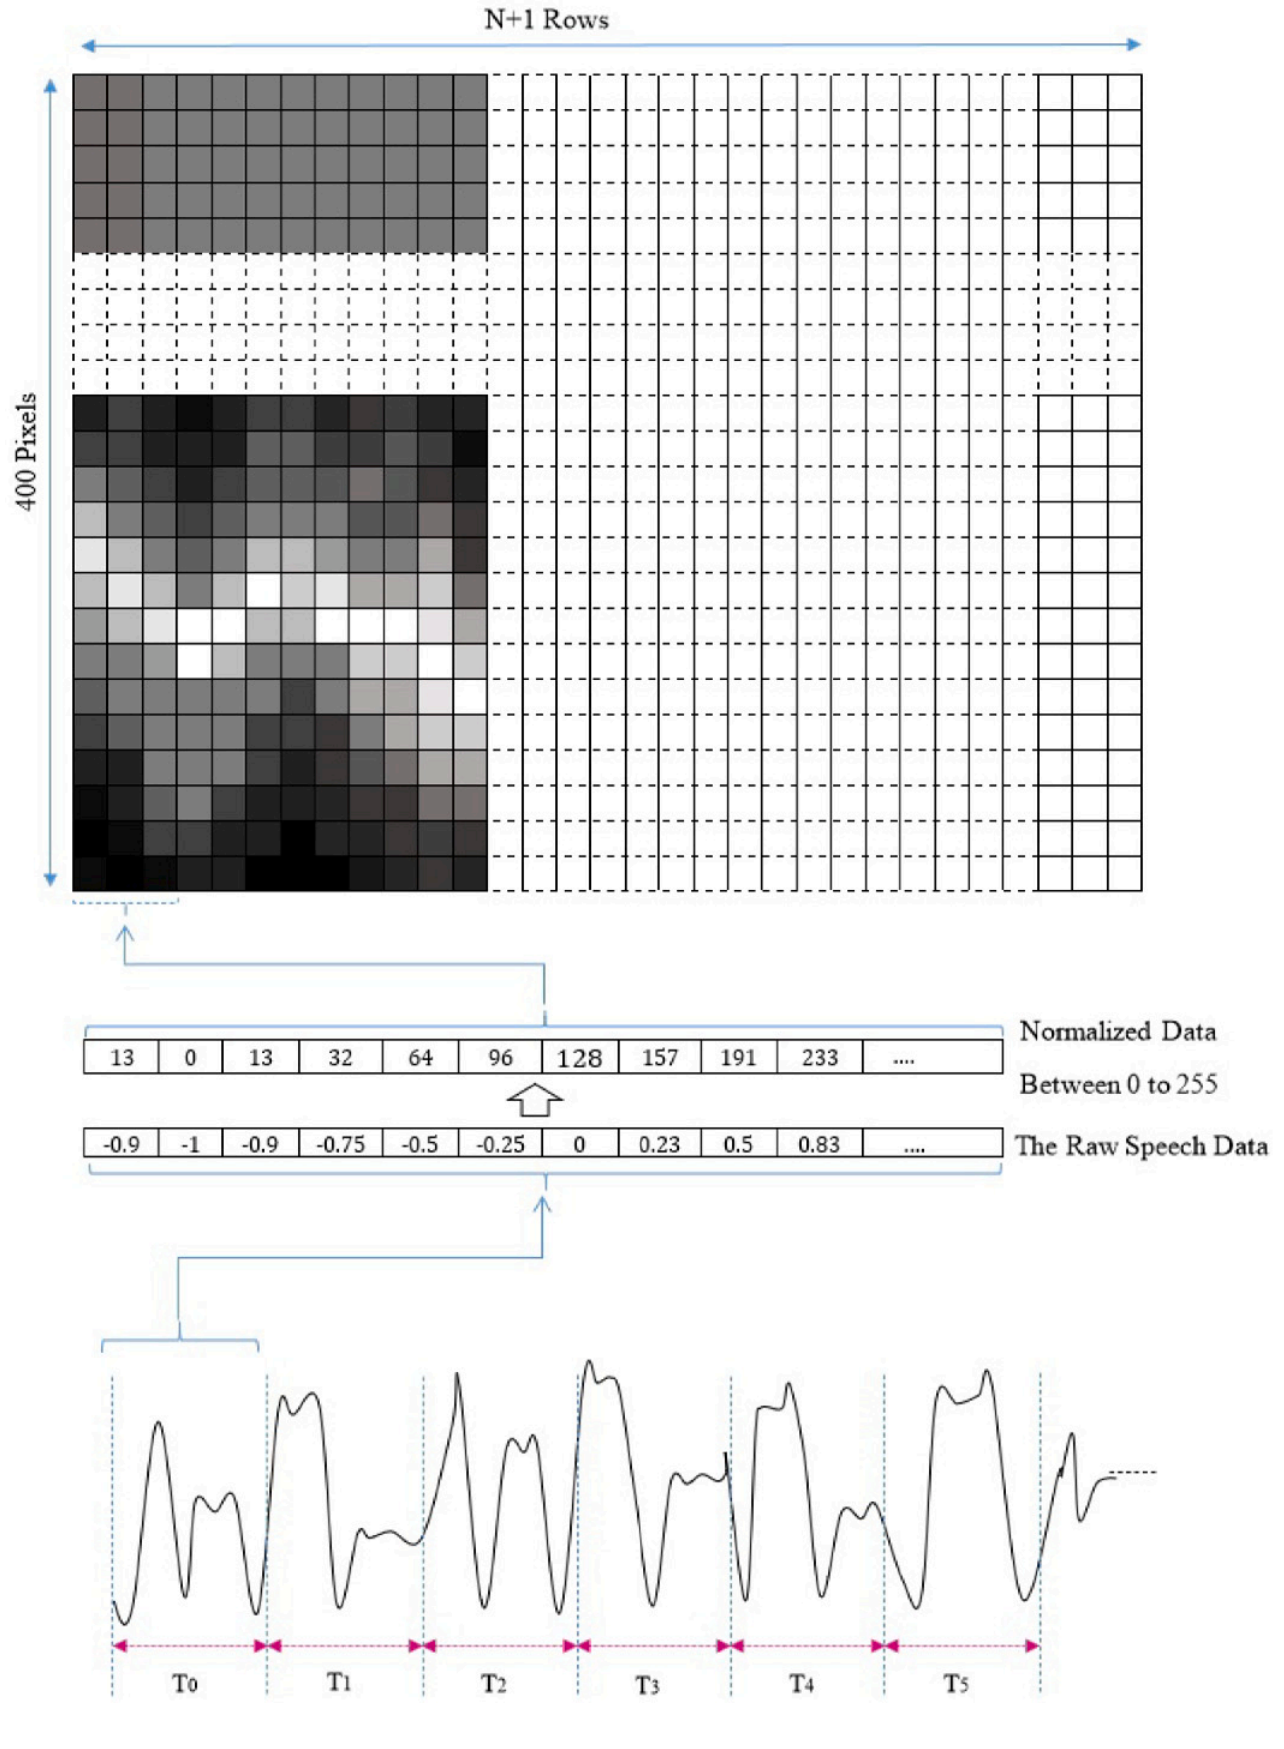
\includegraphics[scale = 1.2]{images/CyTex-diagram.png}
        \caption{CyTex mapping visualized \cite{CyTexRef}}
        \label{cytexVis_example}
\end{figure}

\subsection{RGB Texturing the Image}
Following this, the gradients of the image are calculated. If one was to imagine what these would correspond to in an acoustic sense, one may liken them to the concavity of the function in time. This would be akin to the change in the audio signal over time. For example, is the pitch of the signal trending in an ascending or descending fashion over time. They also apply some form of continuity and interrelation between separate window analysed singals. The results of these calculations are used as the remaining channels of the three channel RGB image. This portion is also another area of interest for innovation. By finding further information about the signal one can increase the dimension of output CyTex objects. This will encode more information in machine network inputs and improve the classification results. 


% SECTION:
% ================================================
\section{Train and Test Databases for SER}
As this genre of task is one of supervised classification, results are dependent on quality labelled data. The databases used to train the model have a drastic impact on the model performance. After all, a model is only as good as the data from which it is constructed. Several types of SER databases exist. However, each pose their own problems. These databases are categorised as Acted, Elicited and Natural \cite{surveyCORE1}.
\begin{description}
\item[Acted (Simulated) Speech:]
Acted datasets, as the name suggests, are entirely fabricated. Actors are employed and will usually be reading text from a script in a professional studio environment. The intention is to act out a certain emotional state whilst reading this script. Due to the controlled nature of this recording process, the signal quality is typically high and requires little audio preprocessing. The construction of an acted database is also simple as it is only limited by the number of actors and budget for their employment. The artificial nature of such a recording process does, however, have its disadvantages. Namely, it is believed that an actor cannot effectively emulate a given emotion in a completely natural way. That is to say that there may exist a disparity between the speech of an actor and speech uttered in a spontaneously emotional way \cite{campbell_2000_databases}. Actor's dialog can be prone to exaggeration and other features that detract from realism. These issues pose problems for the adaptation of learned models to real world data. Having been trained on potentially 'unrealistic' data can massively impact a machine's ability to make correct classifications. 

\item[Natural Speech:] These databases are the most representative of a user's real-world interactions. In this format participants are, mostly, unaware of their recording, (at least in terms of being judged on their emotion). Thus, the emotions expressed are entirely realistic at the time of audio capture. For example, the "Speech Under Simulated and Actual Stress" (SUSAS) Database contains the audio recordings of participants on roller-coasters and in helicopters, among other induced emotional environments, \cite{SUSAS_1997_DB}. While participants may be aware of their own recording, they still demonstrate authentic emotional responses. The drawback of this approach is that there still exists a disparity between these scenarios and everyday situations. In this case, the physical exertion the participant demonstrates is not representative of a typical user's interaction with a machine. There is also significant audio processing to be carried out prior to analysis due to the nature of the recording environment. Due to the nature of recording mostly unaware participants, such a database becomes difficult to construct with any kind of standardised rigor. Legal issues may also arise when considering intellectual property rights and personal confidentiality. Further, deliberately inducing fear and other strong emotions in experiment participants is illegal in many countries \cite{shaver1987emotion}. For these reasons, natural speech emotion databases are often constructed from publicly available audio sources like television and radio. These formats often produce non-ideal audio signals and require some form of preprocessing such as filtering or isolation.

\item[Elicited (Induced) Speech:]
Elicited databases can be viewed as a mixture of the two aforementioned categories. Participants are placed in environments which aim to stimulate specific emotional responses. After the recording process participants self-report the emotions they experienced. This self-reporting as opposed to human labelling is the key differentiating factor between elicited and natural databases. Finally, the aforementioned legal issues which apply to natural speech databases may also apply in this case. 
\end{description}
% --
An important facet of any database used to train the machine learning model is balance. In terms of a classification problem, each output class (emotion) should have roughly the same number of input classes as all other emotions in the training set. However, balance/diversity must also be imposed in terms of other dimensions of the training and test data. For example, the genders of speakers, speaker ages, repetition of phrases using different actors, etc.
Failure to do so will introduce errors into the model like over-fitting for certain types of data and large variance of classification results. This is particularly relevant in the cases of elicited and natural speech databases. Here one must be more selective with the audio used as one no longer has the ability to enforce artificial balance in the dataset. However, The cost of losing balance in the design of speech signals can be compensated by employing a much larger speech library which will contain similar, albeit shorter, acoustic sub-sequences \cite{campbell_2000_databases}.

\subsection{EMODB Database}
The Berlin Emotional Database is an acted emotional speech database spoken entirely in the German language. An acted speech environment was chosen to ensure the controlability and consistency of all elements of the data, apart from manifestations of emotional speech. To remove the bias of a trained actor's emotional exaggeration, roles were advertised openly in the newspaper. From this advertisement 40 people entered the selection phase. An expert panel chose five members of each gender based on their proficiency's in emotional recognisability naturalness of delivery \cite{EMODB_05b_doc}. The ages of participants ranged in between 21 and 35 years of age at the time of recording \cite{EMODB_97}.\\ \\
Choices for dialog were made to minimise the emotional bias the text contained. This can be done via utilising the two following forms of sentences.\\
\textbf{Nonsensical sentences}, which by nature are difficult to associate with any emotions based on the performer's social sensibilities. Unfortunately, the built-in obscurity of such sentences can lead to emotional exaggeration from performers \cite{scherer1981speech}.\\
\textbf{Normal sentences}, which are used so commonly that the performer should be emotionally indifferent to them. These sentences are also simple for actors to rethink in different emotional contexts.\\ \\
\textit{Normal sentences} were chosen for the particular database as "the
use of everyday communication has proved best \cite{scherer1981speech}", due to resembling natural speech when a subject is under emotional stimulation. Ten distinct phrases were spoken and recorded by each actor. Seven distinct emotional states were utilised during the performance process. Each of the phrases and emotions from the dataset are detailed in tables \ref{EMODB_phrase_table} and \ref{EMODB_emo_table}, respectively.
\begin{table}[]
\begin{tabular}{|c|l|l|}
\hline
Code & German Text                            & English Translation                    \\ \hline\hline
a01  & Der Lappen liegt auf dem Eisschrank.   & The tablecloth is lying on the frigde. \\ \hline
a02  & Das will sie am Mittwoch abgeben.      & She will hand it in on Wednesday.      \\ \hline
a04  & Heute abend könnte ich es ihm sagen.   & Tonight I could tell him.              \\ \hline
a05 &
  \begin{tabular}[c]{@{}l@{}}Das schwarze Stück Papier befindet \\ sich da oben neben dem Holzstück.\end{tabular} &
  \begin{tabular}[c]{@{}l@{}}The black sheet of paper is located\\  up there besides the piece of timber.\end{tabular} \\ \hline
a07  & In sieben Stunden wird es soweit sein. & In seven hours it will be.             \\ \hline
b01 &
  \begin{tabular}[c]{@{}l@{}}Was sind denn das für Tüten, die da \\ unter dem Tisch stehen?\end{tabular} &
  \begin{tabular}[c]{@{}l@{}}What about the bags standing \\ there under the table?\end{tabular} \\ \hline
b02 &
  \begin{tabular}[c]{@{}l@{}}Sie haben es gerade hochgetragen und\\  jetzt gehen sie wieder runter.\end{tabular} &
  \begin{tabular}[c]{@{}l@{}}They just carried it upstairs and\\ now they are going down again.\end{tabular} \\ \hline
b03 &
  \begin{tabular}[c]{@{}l@{}}An den Wochenenden bin ich jetzt immer\\  nach Hause gefahren und habe Agnes besucht.\end{tabular} &
  \begin{tabular}[c]{@{}l@{}}Currently at the weekends I always\\ went home and saw Agnes.\end{tabular} \\ \hline
b09 &
  \begin{tabular}[c]{@{}l@{}}Ich will das eben wegbringen und \\ dann mit Karl was trinken gehen.\end{tabular} &
  \begin{tabular}[c]{@{}l@{}}I will just discard this and then\\ go for a drink with Karl.\end{tabular} \\ \hline
b10 &
  \begin{tabular}[c]{@{}l@{}}Die wird auf dem Platz sein,\\ wo wir sie immer hinlegen.\end{tabular} &
  \begin{tabular}[c]{@{}l@{}}It will be in the place where we\\ always store it.\end{tabular} \\ \hline
\end{tabular}
    \caption{EMODB Simulated Phrases \cite{EMODB_97}}
    \label{EMODB_phrase_table}
\end{table}


\begin{table}[]
    \centering
    \begin{tabular}{|llll|}
    \hline
    \multicolumn{2}{|c|}{English}                                    & \multicolumn{2}{c|}{German}               \\ \hline\hline
    \multicolumn{1}{|l|}{Letter} & \multicolumn{1}{l|}{Emotion}      & \multicolumn{1}{l|}{Letter} & Emotion     \\ \hline
    \multicolumn{1}{|l|}{A}      & \multicolumn{1}{l|}{Anger}        & \multicolumn{1}{l|}{W}      & Ärger (Wut) \\ \hline
    \multicolumn{1}{|l|}{B}      & \multicolumn{1}{l|}{Boredom}      & \multicolumn{1}{l|}{L}      & Langeweile  \\ \hline
    \multicolumn{1}{|l|}{D}      & \multicolumn{1}{l|}{Disgust}      & \multicolumn{1}{l|}{E}      & Ekel        \\ \hline
    \multicolumn{1}{|l|}{F}      & \multicolumn{1}{l|}{Anxiety/Fear} & \multicolumn{1}{l|}{A}      & Angst       \\ \hline
    \multicolumn{1}{|l|}{H}      & \multicolumn{1}{l|}{Happiness}    & \multicolumn{1}{l|}{F}      & Freude      \\ \hline
    \multicolumn{1}{|l|}{S}      & \multicolumn{1}{l|}{Sadness}      & \multicolumn{1}{l|}{T}      & Trauer      \\ \hline
    \multicolumn{4}{|c|}{N = Neutral Emotion} \\ \hline
    \end{tabular}
    \caption{Emotions of the EMODB Dataset \cite{EMODB_97}}
    \label{EMODB_emo_table}
\end{table}


Audio was recorded in an anechoic chamber at the Technical University Berlin, sampled at 48kHz and later sampled down at a rate of 16kHz. The audio is of a high quality and requires little to no processing to improve clarity of the acoustic signals. In total there are 700 labelled emotional acoustic signals (7 emotions, 10 actors, 10 unique phrases). As this database is also open to he public it has found immense popularity in the SER research community. 
% It has been chosen as the prime bench-marking database to grade the performance of the results this study seeks to create.


\subsection{RAVDESS Database}
The Ryerson Audio-Visual Database of Emotional Speech and Song (RAVDESS) is another simulated speech dataset, similar to the EMODB dataset. However, this dataset is recorded entirely with English speaking actors from Ontario, Canada. Also unlike EMODB, the dataset also includes facial expression video recordings of actors whilst performing speech and song. This video footage was not analysed for the purposes of this study, however, as the aim is to perform emotional classification purely from audio signals. Only the audio exclusive signals were utilised from this dataset within this project. RAVDESS also, rather uniquely, includes the performance of emotional song. \\ \\
One of the most attractive factors, which has seen the RAVDESS dataset become a standard in SER, is its size. RAVDESS boasts 7356 multi-modal recordings,, consisting of 4320 speech recordings and 3036 song recordings. This is over 10 times the size of the EMODB dataset. Such a large corpus is ideal for machine learning methods. With larger training and testing sets directly improve training and testing results, generally. These clips are composed of a gender balanced cast of 24 professional actors. Actors are tasked with performing at two different emotional intensities, normal and strong, for each of the emotions detailed in table \ref{rav_emo_table}. The incorporation of different intensities is key, as intensity is one of the most salient indicators of emotion \cite{sonnemans1994structure}. 
\begin{table}[]
    \centering
    \begin{tabular}{|c|c|}
    \hline
    Code & Emotion \\ \hline \hline
    01 & neutral \\ \hline
    02 & calm \\ \hline
    03 & happy \\ \hline
    04 & sad \\ \hline
    05 & angry \\ \hline
    06 & fearful \\ \hline
    07 & disgust \\ \hline
    08 & surprised \\ \hline
    \end{tabular}
    \caption{Emotions of RAVDESS \cite{ravdess_dataset_2018}}
    \label{rav_emo_table}
\end{table}
Professional actors are utilised, as for the other datasets, as \cite{EMODB_05b_doc} details that the most identifiable emotional performances are created by actors. Actors were selected from the Toronto, Ontario region of Canada. Interestingly, this region's accent does not prominently exhibit a feature of the Canadian accent known as "Canadian raising" \cite{ravdess_journal}. This phenomena was also avoided via appropriate selection of the stimulus statements. These stimulus statements consisted of two sentences. Firstly, "Kids are talking by the door", and secondly, "Dogs are sitting by the door." These are both examples of \textit{normal sentences}, which the EMODB dataset also makes use of. The studio recording environment is displayed in figure \ref{ravdessstudio}. The complete process of the construction and validation of the RAVDESS dataset is illustrated in figure \ref{ravdessFlowchart}.\\ \\
It is important to note the naming convention of files in the RAVDESS dataset. The filenames are used to distinguish the characteristics of different samples. They are key for separating data points into different classes of emotions, prior to training a deep learning model. Characteristic identifiers are separated by hyphens and are ordered: Modality–Channel–Emotion–Intensity–Statement–Repetition–Actor. Table \ref{rav_code_table} comprehensively highlights the filename identifiers and the characteristic associated with each.
\begin{table}[]
    \centering
    \begin{tabular}{|l|l|}
    \hline
    Identifier & Coding Description of Factor Levels          \\ \hline\hline
    Modality   & 01=Audio-video, 02=Video-only, 03=Audio-only \\ \hline
    Channel    & 01=Speech, 02=Song                           \\ \hline
    Emotion   & \begin{tabular}[c]{@{}l@{}}01=Neutral, 02=Calm, 03=Happy, 04=Sad, 05=Angry,\\ 06=Fearful, 07=Disgust, 08=Surprised\end{tabular} \\ \hline
    Intensity  & 01=Normal, 02=Strong                         \\ \hline
    Statement & \begin{tabular}[c]{@{}l@{}}01="Kids are talking by the door.",\\ 02="Dogs are sitting by the door."\end{tabular}                \\ \hline
    Repetition & 01=First, 02=Second                          \\ \hline
    Actor      & 01=First actor, ..., 24=Twenty-fourth actor  \\ \hline
    \end{tabular}
    \caption{Code Protocol of RAVDESS \cite{ravdess_dataset_2018}}
    \label{rav_code_table}
\end{table}

\begin{figure}
    \centering
    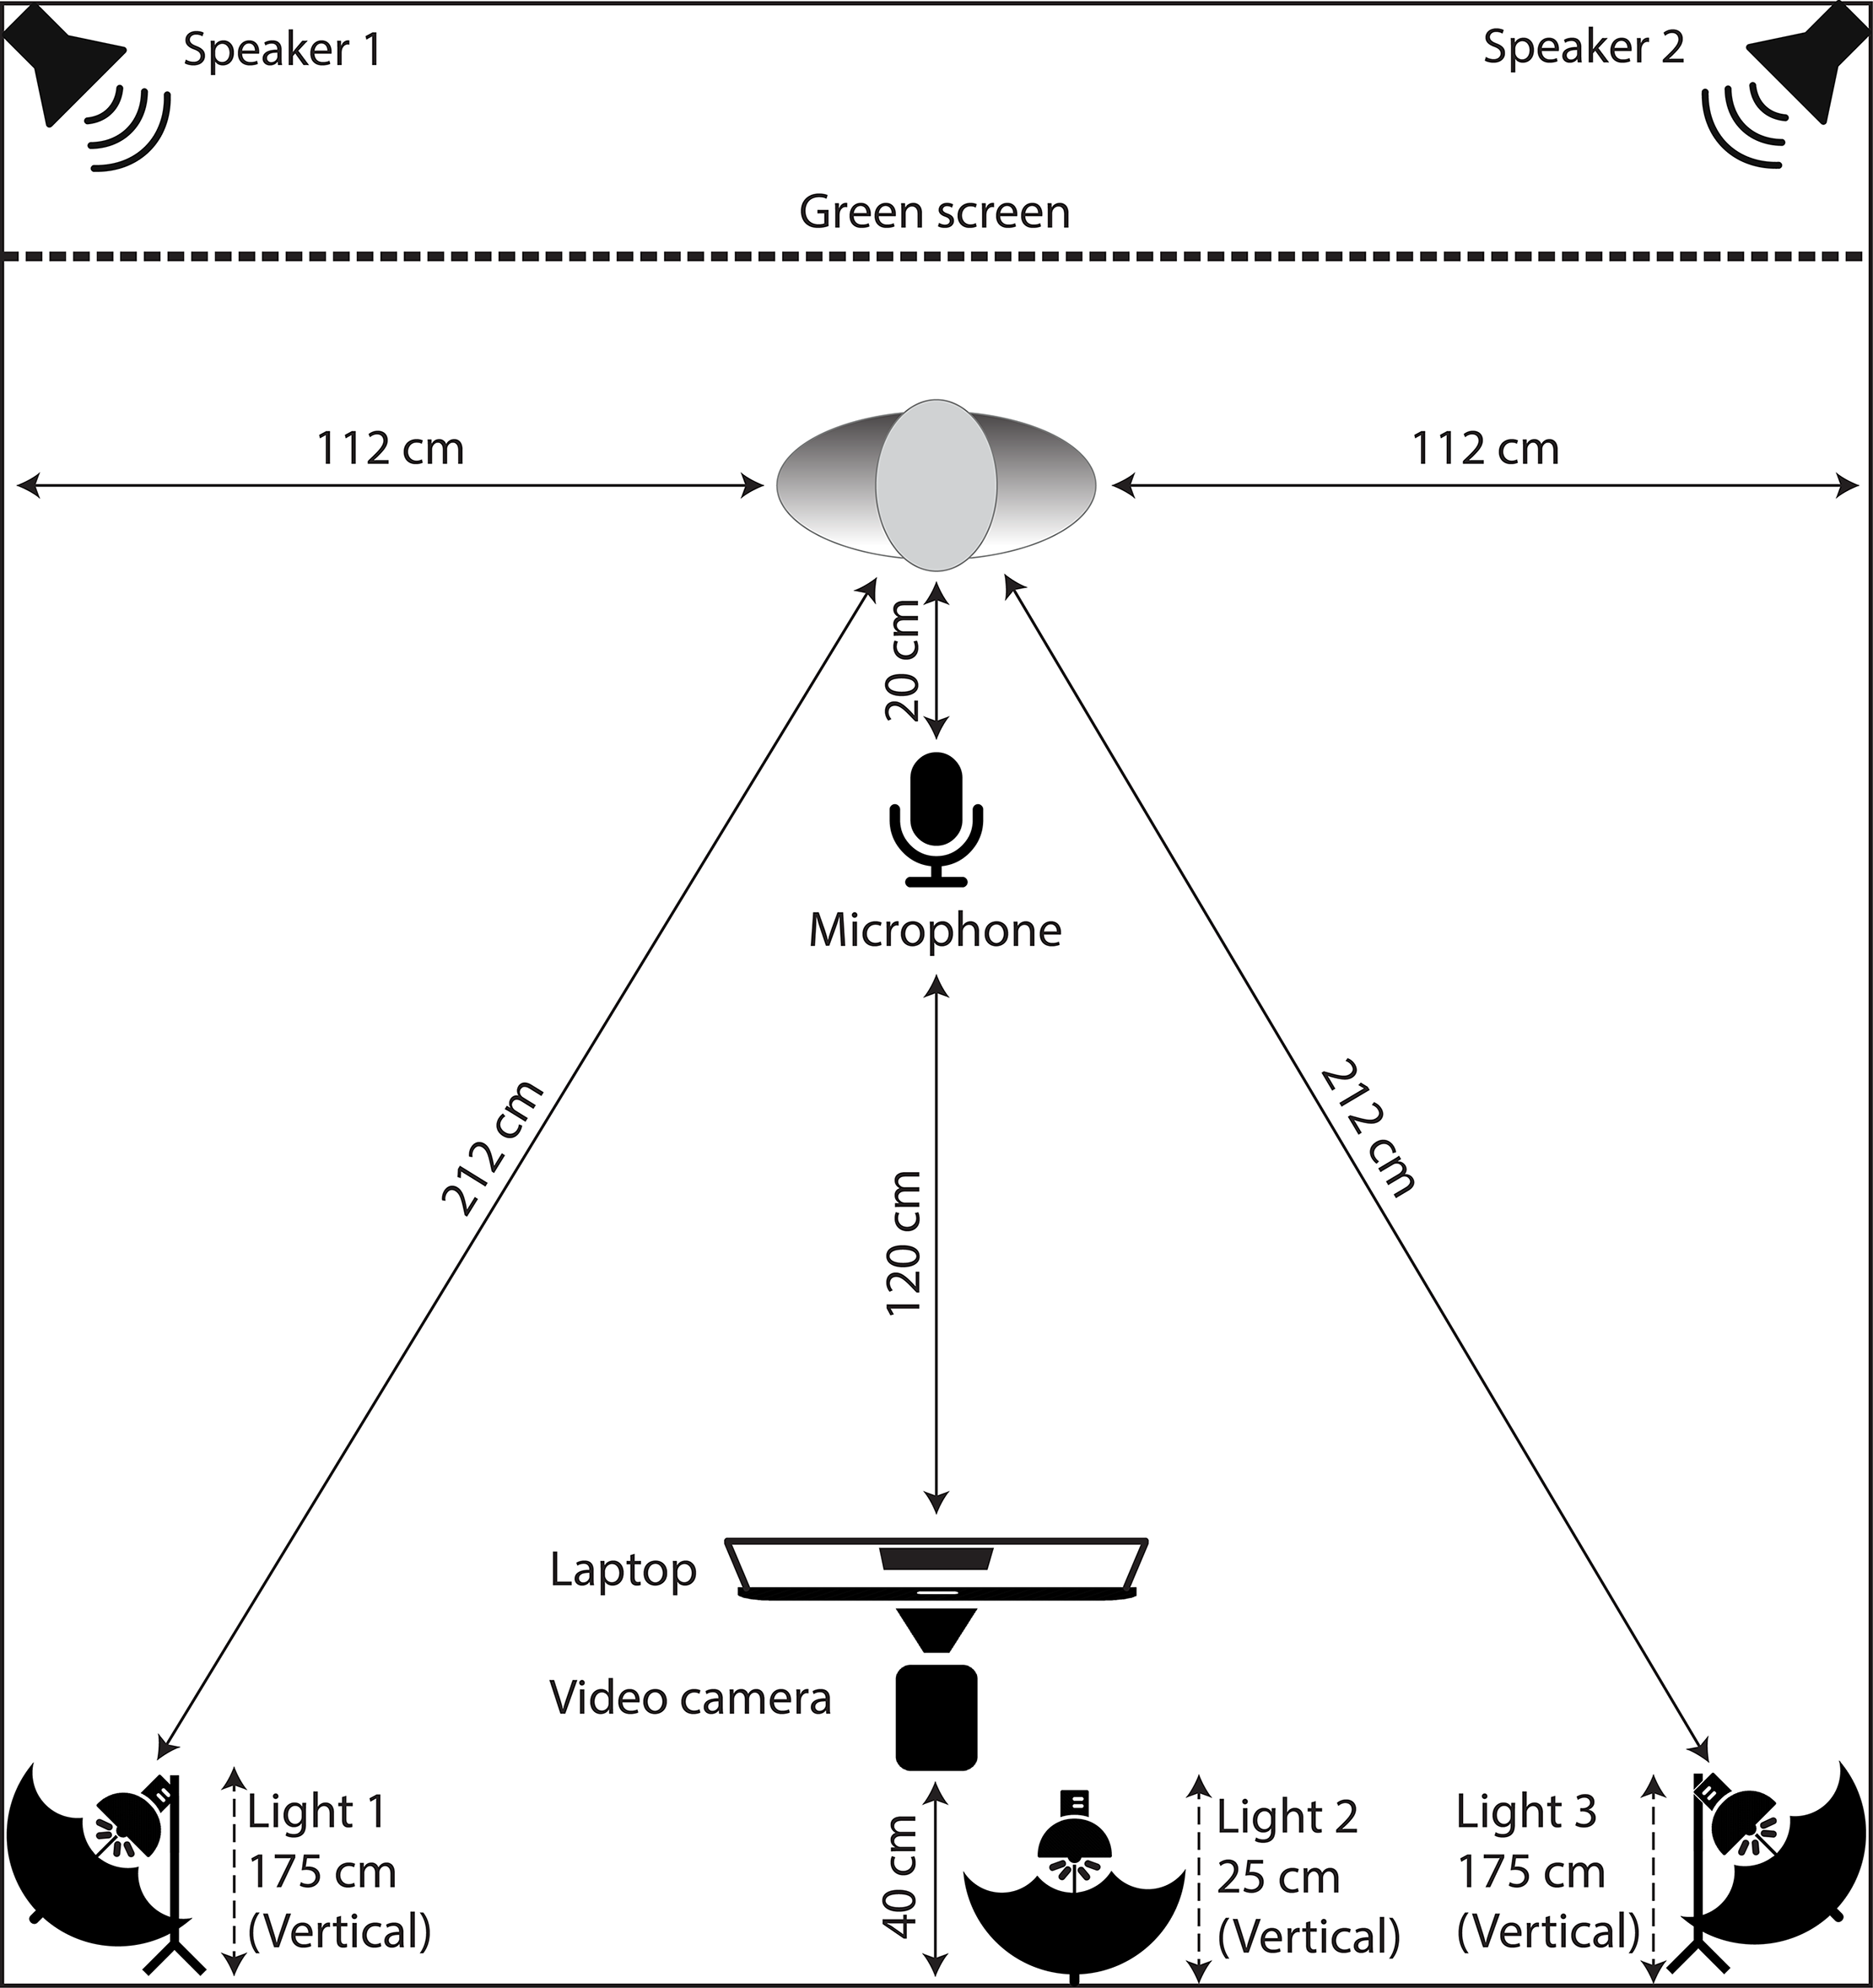
\includegraphics[scale = 0.4]{images/RAVDESS_studioSetup.png}
    \caption{RAVDESS recording environment \cite{ravdess_journal}}
    \label{ravdessstudio}
\end{figure}

\begin{figure}
        \centering
        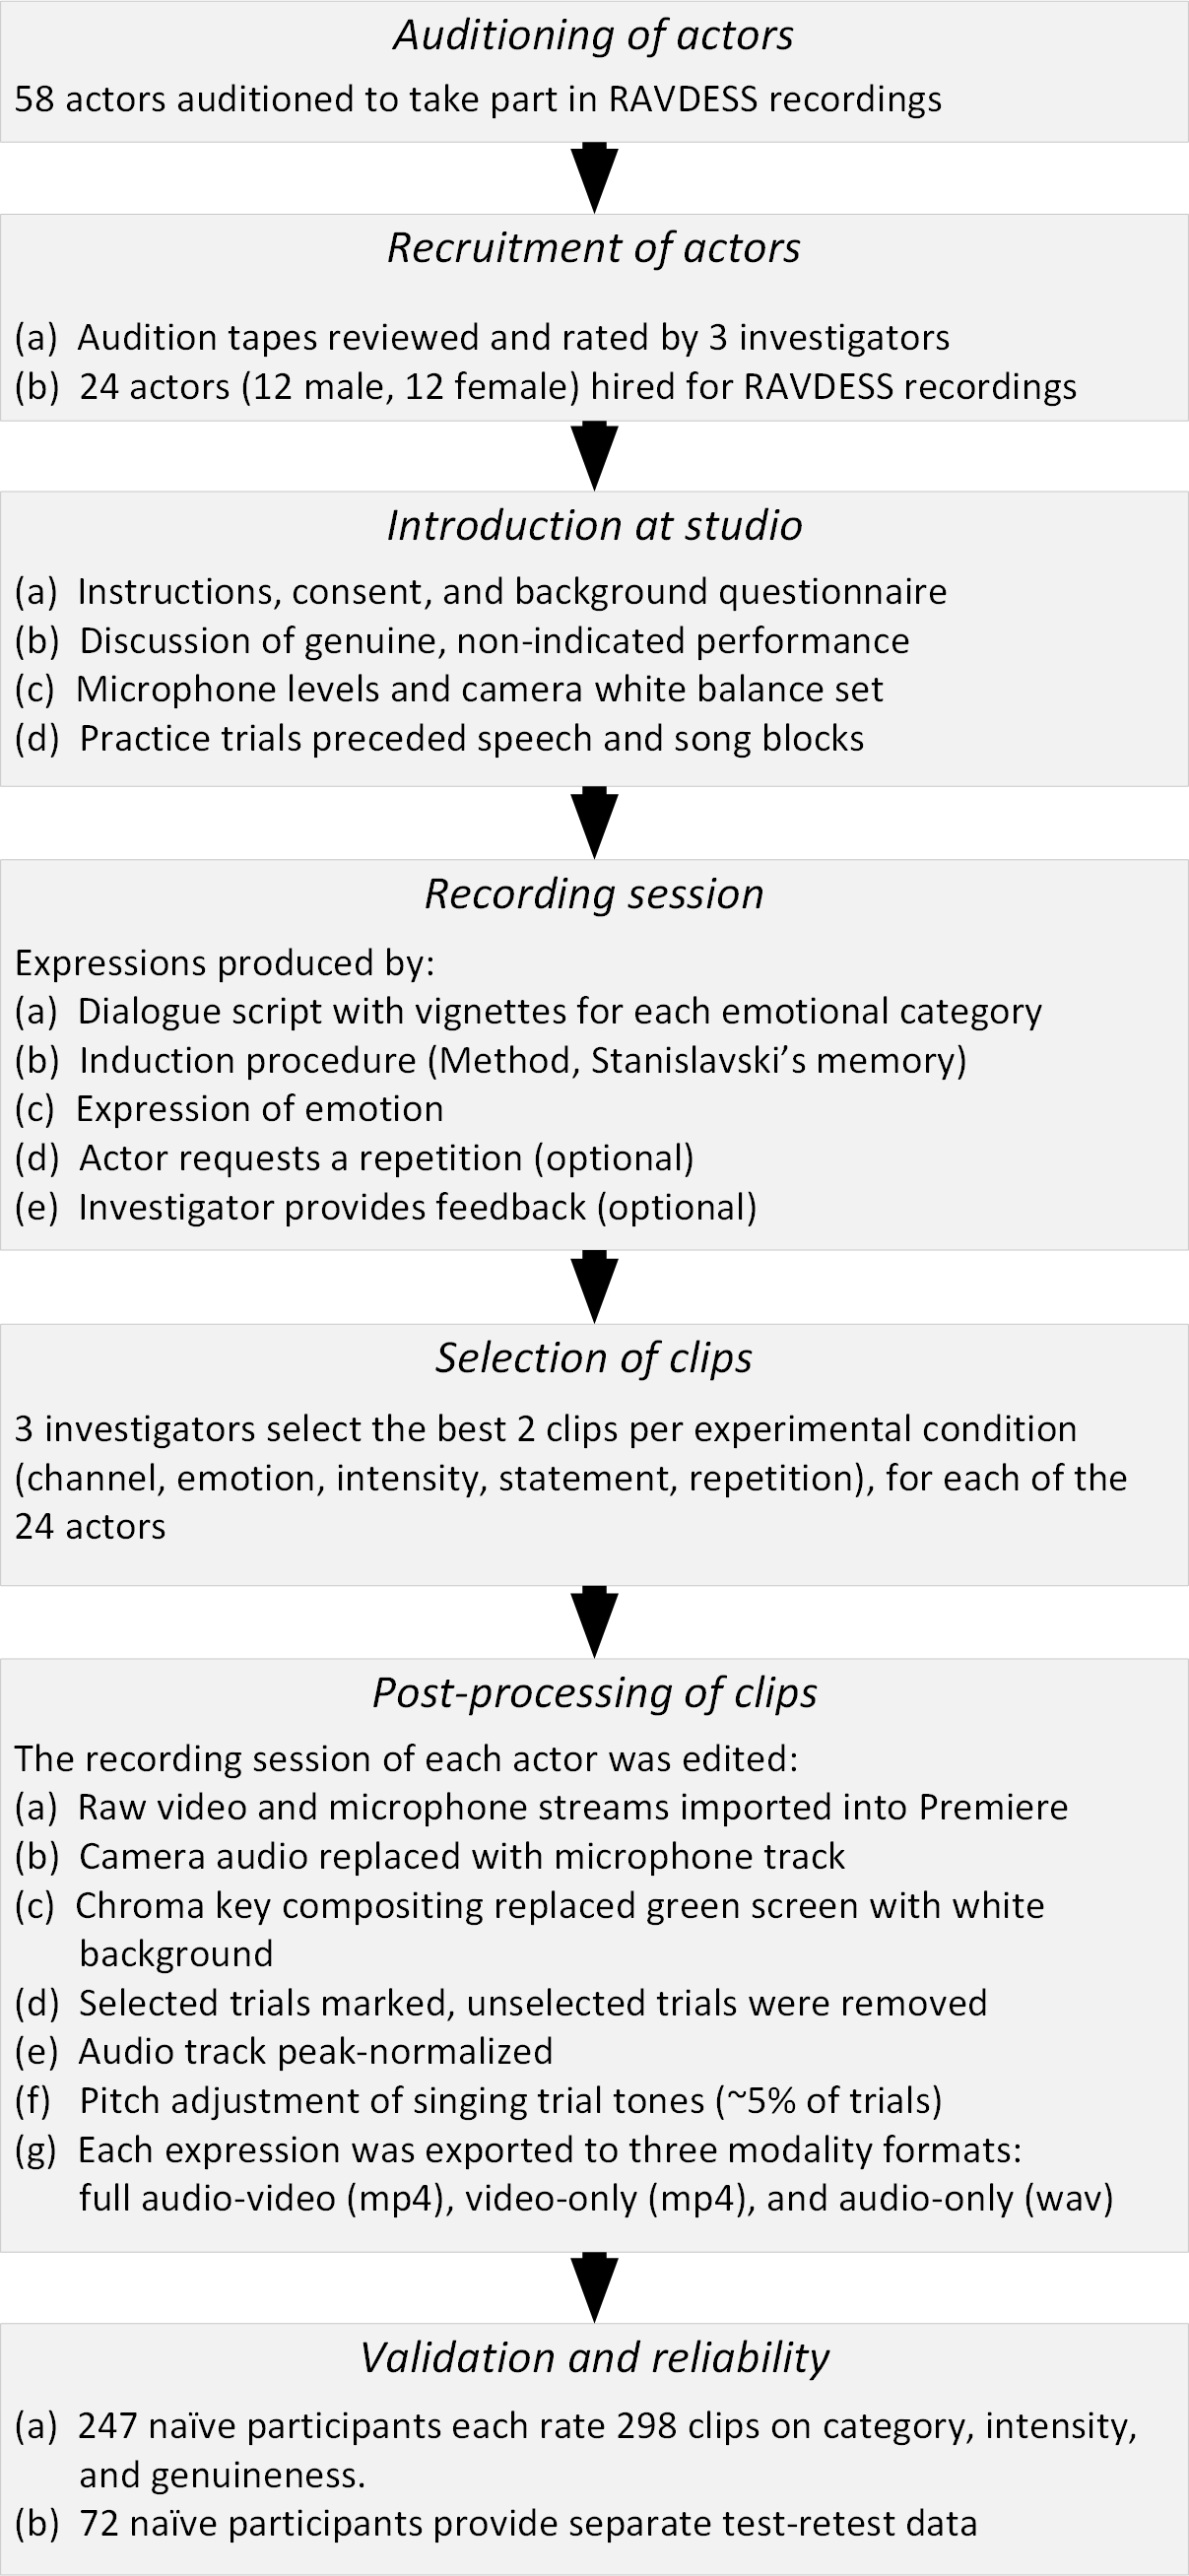
\includegraphics[scale = 1.0]{images/RAVDESS_process.png}
        \caption{RAVDESS construction flowchart \cite{ravdess_journal}}
        \label{ravdessFlowchart}
\end{figure}


\subsection{IEMOCAP Database}
This dataset, while not directly used for the gathering of results in this report, was used in the original CyTex research paper \cite{CyTexRef}. This was motivated by the fact that the RAVDESS dataset had not been previously tested. Instead, the RAVDESS dataset was used.\\ \\
The Interactive Emotional Dyadic Motion Capture (IEMOCAP) Database was constructed is a widely used and accepted benchmark dataset for SER. One of the distinguishing features of this dataset is the wealth of different modalities accessible. Like the RAVDESS, both speech and video are employed. However, modalities like facial motion capture, head angle, head movement, and dialog transcriptions are also available. The dataset was created with the intent to expand research in the areas of gesture and speech relationships, as well as linguistics and communications goals \cite{IEMOCAP_doc}.\\ \\
While the IEMOCAP database is primarily comprised of simulated speech, actors are also given hypothetical scenarios in which their dialog is entirely improvised. This is done with the intent of eliciting emotions from the actor, hence increasing emotional genuineness. In total 10 actors (5 male and female) were used for the recording of this dataset. The spoken language demonstrated throughout is English. Recording was conducted in pairs of actors (dyadic recording sessions). The total accumulated time of all data samples is roughly 12 hours. A relatively standard set of emotions are used in IEMOCAP. This set of emotions are listed in table \ref{iemocap_emo_table}.\\ \\
\begin{table}[]
    \centering
    \begin{tabular}{|c|}
    \hline
    Emotion \\ \hline \hline
    happiness \\ \hline
    anger \\ \hline
    sadness \\ \hline
    neutral \\ \hline
    frustration \\ \hline
    \end{tabular}
    \caption{Emotions of IEMOCAP}
    \label{iemocap_emo_table}
\end{table}
Two different material selection approaches were chosen throughout the recording process. As mentioned prior, improvised scenarios were used to provide some form of induced emotional speech. More conventionally, scripted dialog was exerted from plays was also used, demonstrating simulated speech. This later form offers control over experiment and recording parameters, while the unscripted recordings allow for generalizability to authentic emotions. Each of the play exerts contain verbal interaction between a singular male and female only. These recordings more closely approximate genuine emotion given the greater context of the play \cite{IEMOCAP_doc}. The improvised recordings stemmed from a set list of hypothetical scenarios proposed by \cite{scherer1986experiencing} and detailed in table \ref{iemocap_scenario_table}.
\begin{table}[]
\centering
\begin{tabular}{l|l|l|}
\cline{2-3}
 & Subject 1 (with markers) & Subject 2 (without markers) \\ \hline\hline
\multicolumn{1}{|l|}{1} & \begin{tabular}[c]{@{}l@{}}(Fru) The subject is at the Department \\ of Motor Vehicles (DMV) and he/she is\\ being sent back after standing in line for\\ an hour for not having the right forms of IDs.\end{tabular} & \begin{tabular}[c]{@{}l@{}}(Ang) The subject works\\ at DMV. He/she rejects\\ the application.\end{tabular} \\ \hline
\multicolumn{1}{|l|}{2} & \begin{tabular}[c]{@{}l@{}}(Sad) The subject, a new parent, was called\\ to enroll in the army in a foreign country. \\ He/she has to separate from his/her spouse\\ for more than 1 year.\end{tabular} & \begin{tabular}[c]{@{}l@{}}(Sad) The subject is\\ his/her spouse and is \\ extremely sad for the\\ separation.\end{tabular} \\ \hline
\multicolumn{1}{|l|}{3} & \begin{tabular}[c]{@{}l@{}}(Hap) The subject is telling his/her friend \\ that he/she is getting married.\end{tabular} & \begin{tabular}[c]{@{}l@{}}(Hap) The subject is\\ very happy and wants\\ to know all the details\\ of the proposal. He/she\\ also wants to know the\\ date of the wedding.\end{tabular} \\ \hline
\multicolumn{1}{|l|}{4} & \begin{tabular}[c]{@{}l@{}}(Fru) The subject is unemployed and \\ he/she has spent the last 3 years looking\\ for work in his/her area. He/she is \\ losing hope.\end{tabular} & \begin{tabular}[c]{@{}l@{}}(Neu) The subject is \\ trying to encourage\\ his/her friend.\end{tabular} \\ \hline
\multicolumn{1}{|l|}{5} & \begin{tabular}[c]{@{}l@{}}(Ang) The subject is furious, because\\ the airline lost his/her baggage and \\ he/she will receive only \$50 (for a \\ bag that cost over \$150 and has lots \\ of important things).\end{tabular} & \begin{tabular}[c]{@{}l@{}}(Neu) The subject works\\  for the airline. He/she tries\\ to calm the customer.\end{tabular} \\ \hline
\multicolumn{1}{|l|}{6} & \begin{tabular}[c]{@{}l@{}}(Sad) The subject is sad because a\\ close friend died. He had cancer that\\ was detected a year before his death.\end{tabular} & \begin{tabular}[c]{@{}l@{}}(Neu) The subject is trying\\ to support his friend in this\\ difficult moment.\end{tabular} \\ \hline
\multicolumn{1}{|l|}{7} & \begin{tabular}[c]{@{}l@{}}(Hap) The subject has been accepted\\  at USC. He/she is telling this to \\ his/her best friend.\end{tabular} & \begin{tabular}[c]{@{}l@{}}(Hap) The subject is very\\ happy and wants to know\\ the details (major, scholarship).\\ He/she is also happy because \\ he/she will stay in LA so\\ they will be together.\end{tabular} \\ \hline
\multicolumn{1}{|l|}{8} & \begin{tabular}[c]{@{}l@{}}(Neu) He/she is trying to change\\ the mood of the customer and\\ solve the problem.\end{tabular} & \begin{tabular}[c]{@{}l@{}}(Ang) After 30 min talking\\ with a machine, he/she is\\ transferred to an operator.\\ He/she expresses his/her \\ frustration, but, finally, he/she\\ changes his/her attitude.\end{tabular} \\ \hline
\end{tabular}
    \caption{Scenarios of IEMOCAP \cite{IEMOCAP_doc}}
    \label{iemocap_scenario_table}
\end{table}
IEMOCAP audio was recorded using a dual microphone setup, (one microphone per actor). Audio was sampled at a frequency of $48kHz$. To prioritize depth of emotion it was required that the two interacting actors were visible to each other. Camera and microphone equipment was positioned to accommodate this.

% SECTION:
% ================================================
\section{Deep Learning Fundamentals}
This section details the fundamental concepts necessary for understanding and applying methods of deep learning in the context of this project. Beginning with motivations of deep learning and traversing theoretical key concepts. One should note, however, that this review is by no means comprehensive. This section merely addresses the required material for understanding subsequent strategies and results of this report.\\ \\

\subsection{The Motivation For Deep Learning}
Problems in the domain of Artificial Intelligence (AI) are generally solved by generating an appropriate set of features to describe trends in a dataset. These features are input into a simple machine learning algorithm. Having analysed these features, the machine learning model can use this information to predict, classify, or make any number of assessments on a dataset. However, it may not be apparent which features best inform an algorithm, or which may be easily extracted. This introduces the concept of \textit{representation learning}. Representation learning utilises machine learning to not only learn patterns in data, (mapping features to outputs), but to learn the very features as well. \textit{Deep Learning} then refers to a sub-branch of representation learning in which complex features of a dataset are created hierarchically from simpler features. An example highlighting the development of complex features based upon simpler variants is illustrated in figure \ref{DL_feature_fig}. The need for deep learning comes about when finding complex features becomes as, or more, challenging than the initial machine learning problem one was trying to solve. One of the key advantages of deep learning is that the more data a model sees, the more complicated features it can build from simpler ones, improving performance. Another asset is the elimination of feature design. The user need not inform the computer of which features are important to determine an output, as the model will learn this itself through the training procedure.
\begin{figure}
        \centering
        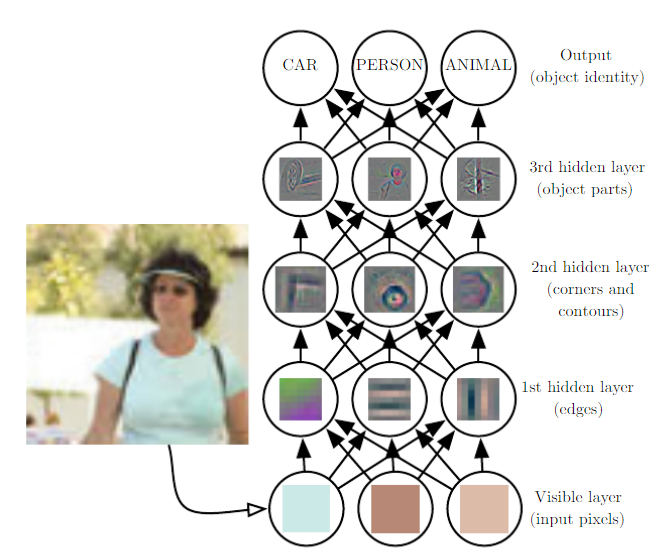
\includegraphics[scale = 0.7]{images/DL_features_figure.png}
        \caption{Deep learning feature generation \cite{Goodfellow-et-al-2016}}
        \label{DL_feature_fig}
\end{figure}

\subsection{Machine Learning - Key Concepts}
\subsubsection{Components of Learning}
The phrase 'Machine Learning' consists of two fundamental components we must understand. Where a machine simply refers to a computer, learning is defined more rigorously. To define learning we first introduce three concepts; a task (\textit{T}), performance measure (\textit{P}), and experience (\textit{E}).\\ \\
Firstly, a task \textit{T} is some action or process we wish to perform. Popular examples in contemporary literature include classification, anomaly detection, and regression. Initially, the computer may have no way of executing a process to complete some task. This is where experience \textit{E} enters. Experience refers to the scrutiny of a dataset and the machines interaction with the dataset during this process. This study approaches experience from a \textit{supervised} perspective. That is to say that a supervised learning algorithm experiences the dataset. In this setting example data \textbf{x} is associated with some target value \textbf{y}. The experience of the machine is used to inform the estimation of $p(y|x)$. In other words, finding a relating mapping between an input and provided output. Another setting, not discussed in this work, is that of \textit{unsupervised learning}. Here \textbf{x} is given, however no corresponding output \textbf{y} will be provided to the machine. The machine instead attempts to learn the underlying probability distributions of groups of example data. Finally, the performance measure \textit{P} is a user defined metric which attempts to grade how well an algorithm performs at a given task \textit{T}. The most obvious grading for many models is some indication of accuracy, expressed as a ratio of correct predictions to total predictions made.

\subsubsection{Defining Learning}
Having defined the building blocks of learning, we may now formally define learning by the definition provided by \cite{mitchell_97_ML}. Mitchell poses, “A computer program is said to learn from experience \textit{E} with respect to some class of tasks \textit{T} and performance measure \textit{P}, if its performance at tasks in \textit{T}, as measured by \textit{P}, improves with experience \textit{E}.”

\subsubsection{Generalization and Model Fitting}
Another concept at the core of machine learning is that of \textbf{Generalization}. This refers to model performance graded on data inputs which do not belong to the training set used to learn the model. Generalization is important as any model is essentially useless if it cannot perform its intended function on input data it has not seen before. In the pursuit of attaining sufficient model generalization, one must be weary of two undesirable phenomena, \textit{underfitting} and \textit{overfitting}. Underfitting implies that the model has not sufficiently been trained and cannot extract enough meaning from the training data to perform its intended task. Overfitting, conversely, refers to giving the model too much exposure to training data. In this case, a model may be memorizing training data, as opposed to intelligently identifying prominent features and characteristics of the data. This typically results in large training accuracy and poor generalization (low test and validation accuracy). Both of the phenomena can be visualized in figure \ref{biasVarTrade}. Here the capacity informally refers to a model's ability to broadly fit many functions \cite{Goodfellow-et-al-2016}. It can be seen that as capacity increases the training error, (approximately indicated by bias), decreases. However, the generalization error after some point begins to increase. This indicates that there is some optimal point at which one should stop training a machine learning model to optimise generalizability.
\begin{figure}
    \centering
    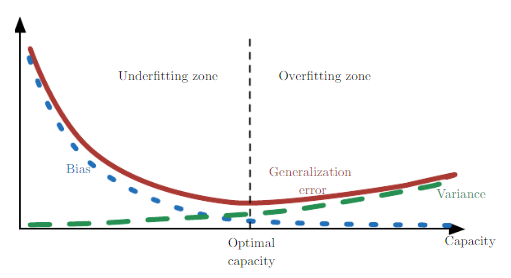
\includegraphics[scale = 1.0]{images/BiasVarTradeOff_Fig.png}
    \caption{Bias variance trade-off and model fitting \cite{Goodfellow-et-al-2016}}
    \label{biasVarTrade}
\end{figure}

\subsubsection{Bias and Variance}
In defining bias and variance, we first define a point estimator of some parameter $\pmb{\theta}$ as in equation \ref{pointEst_eq}. Here each $\pmb{x}$ is an independent and identically distributed (i.i.d.) data point.
\begin{equation}
    \hat{\pmb{\theta}}_m = g(\pmb{x}^{(1)}, ..., \pmb{x}^{(m)})
    \label{pointEst_eq}
\end{equation}
Bias may then be defined by equation \ref{bias_eq}.
\begin{equation}
    bias(\hat{\pmb{\theta}}_m) = \mathrm{E}(\hat{\pmb{\theta}}_m) - \pmb{\theta}
    \label{bias_eq}
\end{equation}
That is to say the bias is given by the difference between the expected value of the point estimator of some parameter and the true underlying value of that parameter. An estimator is called unbiased if, in this case, equation \ref{bias_eq} equates to zero. In a machine learning context, bias gives an indication of how well a model understands the data and its characteristics within a training set. It measures the 'distance' (or error) between a prediction and some actual value. For this reason it is optimal to minimise bias , although only to a point (refer to figure \ref{biasVarTrade}).\\ \\
One must also consider the variance of an estimator. Variance indicates how sensitive a model is to perturbations within the training set. The variance of an estimator is defined in terms of conventional statistical variance, see equation \ref{var_eq}.
\begin{equation}
    Var(\hat{\theta})
    \label{var_eq}
\end{equation}
As is noted above, variance gives indication of a model's performance on unseen data. For this reason the variance is related to model generalizability. By referring to figure \ref{biasVarTrade}, one may note a compromise that must be made between suitably low bias and variance. This concept is know as the \textbf{bias variance trade-off}. In other words, improvements in training accuracy beyond a certain point sacrifice the extent to which a model can generalize. In this study the trade-off is handled via implementation of cross-validation. 

\subsubsection{Cross-Validation}
A typical split of data involves using $80\%$ of a dataset to create a training set and the remaining $20\%$ to create a test set. One can imagine the motivation of these choices, as a model needs to be exposed to as much data as possible to learn defining characteristics of a dataset. However, a sufficiently large subset must remain for testing to any kind of meaningful results. For smaller datasets, division of the net dataset into train and test sets can introduce uncertainty into the test results of a model. A small test set is akin to an insufficient sample that does not accurately represent the complete dataset. For this reason, along with the ubiquity of smaller than ideal datasets, alternate methods of determining test error performance have been developed.\\ \\
Of particular interest to this study is the method of \textit{k-fold cross validation}. This method partitions datasets into random training and test sets  and executes the training process. After this is complete the training process begins again, however, a different partitioning of the dataset is used to construct the train and test subsets. The name of this method comes from the splitting of the data in subset creation. Data is split into \textit{k} partitions containing no overlapping elements. Of these \textit{k} sets, one will be used as the test set and the remainder will be used for training. Following this, the test set will be iterated to the next partition of data and training will be commenced upon the remaining subsets once more (now including the test set from the previous iteration). This process is executed \textit{k} times and the results of each trial are stored and then averaged.

\subsection{The Classification Problem}
% \subsubsection{Defining Classification}
Classification is the basis of many interesting modern artificial intelligence applications. Be it object recognition employed in driverless cars, or medical diagnosis from particular medical imaging datasets.\\ \\
This task involves specification of an input in terms of it belonging to some group. Each of these groups may be referred to as \textit{classes} or \textit{targets}. A model is trained to develop some mapping function which takes an input and maps it to the most probable class that said input belongs to. This mapping function is notated as $f: \mathbb{R}^n \rightarrow \{1, ..., k\}$ for $k$ number of classes. Outputs may vary depending on the construction of the model and type of problem. In the context of this thesis the probability of a particular input belonging to each of the possible emotional classes is used. The maximum is taken of this output to determine the emotional class with the highest probability for the corresponding input.
% \subsubsection{Outputs Using Softmax}
% Get infor from 6.2.2.3 in deep learning (Ian Goodfellow)

% \subsection{Regularization - Methods of Generalization}
% "Regularization is any modification we make to a learning algorithm that is intended to reduce its generalization error but not its training error", \cite{Goodfellow-et-al-2016}.
% \subsubsection{Dataset Augmentation}
% \subsubsection{Training and Early Stoppage}
% \subsubsection{Dropout}

% \subsection{Model Optimization}
% % TIME PERMITTING:
% % \subsubsection{Minibatch Stochastic Optimization}
% \subsubsection{Neural Network Optimization Difficulties}
% % refer to section 8.2
% % TIME PERMITTING:
% % \subsubsection{Parameter Initialization}
% \subsubsection{Stochastic Gradient Descent}
% \subsubsection{ADAM Stochastic Optimization}
% % discussed in textbook but printed paper is main source! Adaptive learning rate method.
% \subsubsection{Batch Normalization}
% refer to printed batch norm academic paper, textbook also discusses.

\subsection{Convolutional Neural Networks}
Convolutional Neural Networks (CNNs) are networks proficient in grid based data processing and analysis. One prominent example is that of an image. An image is a grid consisting of pixels. For some time CNNs have been very popular due to their high performance and ease of production, given many open source tools and packages exist to aid in their construction. 

\subsubsection{Convolution}
Convolution can be defined in terms of two functions in time, $f(t)$ and $h(t)$. The convolution of these two functions is shown in equation \ref{convolution_eq}.
\begin{equation}
    f(t) * h(t) = \int f(\tau)h(t-\tau) d\tau
    \label{convolution_eq}
\end{equation}
The operation of convolution can also be thought of graphically. The function $h$ is flipped about the y-axis and progressively shifted to the right as the $t$ parameter increases. As this function is shifted, the integral of the multiplied functions is calculated. In equation \ref{convolution_eq}, $f$ may be referred to as the input and $h$ is the kernel or filter. The output of this operation constitutes the interaction between $f$ and $h$ (the input and some filter). This output may be known as the feature map.\\ \\
Due to the nature of signal processing and machine learning taking place in a digital setting, it make sense to discretize this process. Just as was done for in the continuous case, we define discrete time convolution as in equation \ref{disc_conv_eq}.
\begin{equation}
    f[k]*h[k] = \sum^{\infty}_{m=-\infty} f[m]h[k-m]
    \label{disc_conv_eq}
\end{equation}
One may note that the graphical explanation for continuous time convolution still holds in this case. The key difference in discrete time is that the integral of the multiplied functions is no longer calculated. Now, the summation of all multiplied overlapping discrete instances are calculated. 

\subsubsection{Convolution in the Image Domain}
In image processing, the input $f$ will be a tensor representing the input image. The filter $h$ will be some arbitrarily sized tensor of values chosen to appropriately scale the input under convolution. We will label the input image $I$ and the filter (or kernel) as $K$, following the conventions set in \cite{Goodfellow-et-al-2016}. Both of these objects are two-dimensional. The convolution of these objects is defined by equation \ref{2d_conv_eq}.
\begin{equation}
    (I*K)(i, j) = \sum_m\sum_n I(m,n)K(i-m, j-n)
    \label{2d_conv_eq}
\end{equation}
As the filter is now in two-dimensional space, the graphical explanation must be altered slightly. Instead of 'flipping' the filter about the y-axis, as was performed in the on-dimensional case, we must flip the filter about two sets of axes. By flipping the filter about x and y, this is the same as taking the 2-D array and rotating it $180^\circ$ counter clockwise. The filter/kernel is the slid across the two-dimensional image and each overlapping pixel value is multiplied and summed.

\subsubsection{Why CNNs Matter}
The usefulness of this operation lies in a filter's ability to extract features from an input. For example, if the input is a 2-dimensional image, by sliding and convoluting some filter over the image, many features may be extracted. Initially the filtering effect may make edges more prominent and allow the learning algorithm to better detect the edges of objects.\\ \\
Another advantage of using these networks is by restricting the type of interactions between outputs and inputs in convolutional layers. Since the kernel is smaller than an input image, when sliding it over we can detect things in smaller regions. This also results in more efficient computation than matrix multiplication based methods. These kinds of interactions are referred to as \textit{sparse interactions}.\\ \\
Unlike traditional neural networks, CNNs also offer shared parameters. By using shared parameters, less parameters overall need be learned, reducing the net required storage for the learned model.

% \subsubsection{Pooling}


% SECTION:
% ================================================
\section{Transfer Learning - Economic Model Building}
Transfer Learning refers to the process of re-purposing pre-trained deep learning models. These models are initially trained for some problem, and later applied to an adjacent task. In doing so, one can leverage the power of the initial model and save time and computational effort. This process may also improve generalization of the final model. In essence, transfer learning utilises powerful models as starting points to extend upon. 

\subsection{Transfer Learning Basics}
Strategies of machine learning typically employ a training dataset which is used to teach a model patterns in the data. Validation of the learnt model is performed on a test set. Both of these datasets usually have the same feature space and data distribution. If this is not the case, prediction performance can depreciate \cite{SHIMODAIRA2000}. Transfer learning passes on information, which has already been learnt by a model, to improve another model in a related domain. This approach is necessary when training data is hard to obtain, or its size is insufficient, (as is the case for many emotional audio datasets). SER has historically been a smaller research field of interest and, as has previously been noted, is a lot younger than other machine learning fields. This has caused datasets to have limited access, limited size, or be largely/entirely unlabelled. As one can imagine, because emotion is perceived subjectively by humans, labelling emotional speech data is ill-advised. For these reasons, the employment of transfer learning is hugely beneficial for SER tasks which are solved in the image domain.\\ \\
\textbf{Defining Transfer Learning}\\
To formally define transfer learning, this report uses the conventions in notation and definition of the prominent surveys \cite{IEEE_TL_Survey} and \cite{2016transfer_survey}. Before defining transfer learning, we must first define its constituents. A \textit{domain} $\mathcal{D}$ has some feature space $\mathcal{X}$ and a marginal probability distribution $P(X)$, with the feature space $\mathcal{X}$ containing all feature vectors for a given learning sample $X = \{ x_1, ..., x_n \}$. The domain can be notated $\mathcal{D} = \{ \mathcal{X}, P(X) \}$.\\
A \textit{task} $\mathcal{T}$ is notated as $\mathcal{T} = \{ \mathcal{Y}, f(\cdot) \}$. Here, $\mathcal{Y}$ is the \textit{label space}, and $f(\cdot)$ is an objective predictive function. The objective predictive function is not known, however, by observing trends in training data, a suitable $f(\cdot)$ can be learned such that a label $y$ from instance $x$ can be predicted. In this training data, each $x_i$ is associated with a corresponding $y_i$. Thus, the objective predictive function can be written in conditional probabilistic terms as $f(x) = P(y|x)$.\\
Finally, we can define two different types of associated domains and tasks in the context of transfer learning. The source domain $\mathcal{D}_S = \{ \mathcal{X}_S, P(X_S) \}$ and source task $\mathcal{T}_S = \{ \mathcal{Y_S}, f_S(\cdot) \}$ both stem from some machine learning problem. In this paper's context, the source domain is images and the source task is the classification of objects in those images. The target domain $\mathcal{D}_T = \{ \mathcal{X}_T, P(X_T) \}$ and target task $\mathcal{T}_T = \{ \mathcal{Y_T}, f_T(\cdot) \}$ are also related to some machine learning problem, which may share similarities with the source problem. Again, in the context of this study, the target domain is images. However, the target task is emotional classification. Finally, we define transfer learning as the following.\\ \\
\textit{Given a source domain and learning task, along with target equivalents $\mathcal{D}_S$, $\mathcal{T}_S$, $\mathcal{D}_T$ and $\mathcal{T}_T$, respectively,  transfer learning aims to improve the learning ability of $f_T(\cdot)$ using previously learnt knowledge in $\mathcal{D}_S$ and $\mathcal{T}_S$. In this case either $\mathcal{T}_S \neq \mathcal{T}_T$, or $\mathcal{D}_S \neq \mathcal{D}_T$} \cite{IEEE_TL_Survey}.\\ \\


% WONT HAVE TIME TO INCLUDE :(
% \subsection{Translation of Deep Learning Features}
% \textbf{***Get info from transferable features paper!}\\
% \cite{yosinski2014transferable}\\


% \subsection{CyTex Enabling Transfer Learning}
%  The power of transfer learning is unlocked through mappings like the CyTex transform.


% TALK ABOUT TRANSFER LEARNING. Two different resources to use here. A gentle introduction webpage in bookmarks + use survey, first few pages with definitions.




% ===========================================
%	Chapter 5
% ===========================================
\chapter{SER Simulations and Results}\label{ch-ser_sim}
This section discusses the experimental procedure of using CyTex to generate RGB images and the construction of a DCNN model to extract features and classify the dominant emotion of each CyTex image passed through the model. It is of importance to note that machine learning results can often be hardware dependent and difficult to reproduce, even under the same experimental conditions. The Initial simulation results and improved results are both discussed. This is to inform the reader of the dependency on hardware related to performance. It also highlights the nature of machine learning problems, which often require significant tuning and reconstruction to achieve more desirable results. Through this chapter, the engineering design process should also be acknowledged; making informed decisions and balancing trade-offs to improve system performance. 

% SECTION:
% ================================================
\section{Experimental Environment}
All programming of this project took place in Python. The Integrated Development Environment (IDE) utilised was PyCharm on certain local machines and VSCode in other instances. GitHub was used for centralized version control of the project. The GitHub repository for this project can be accessed through the following reference \cite{Blake_ELEC4840B-Repo}. Further information regarding the structure and functionality of the code can be found in the \textit{readme.md} file of the aforementioned repository.\\ \\
The deep learning component of this thesis was carried out using PyTorch and it's associated deep learning deep learning frameworks \cite{PyTorch_Ketkar_2017}. The office spaces and computers in \textit{ES-219} and \textit{ES-115A} were utilised for preliminary code building and DCNN simulation, respectively. Sufficiently advanced contemporary equipment is required to complete deep learning simulations in a reasonable amount of time. Specifically, deep learning simulations should be conducted on platforms with appropriate graphics cards to enable parallel processing. This hardware not only effects the time of simulations, but also the quality and accuracy of results. IThe hardware specifications of the work station present in \textit{ES-115A} include an Intel Core i7-7800X CPU at 3.5GHz, 2 threads per core and 6 cores per socket. The memory is rated as 32 GB DDR4 memory. Finally, a CUDA enabled graphics card was utilised for deep learning simulation. The graphics card utilised was an NVIDIA GeForce GTX 1080 Ti with a 33MHz clock.

% SECTION:
% ================================================
\section{Generating CyTex Images}
The generation of CyTex images for all databases detailed in this thesis followed the structure highlighted in chapter \ref{ch-theory}, figure \ref{cytexFlowchart}. However, this section gives further specificity with respect to the programming and construction of the process. Choices for important parameters are also discussed.
\subsection{Loading and Resampling}
Initially each of the \textbf{.wav} files are loaded using the glob python library which allows for UNIX based string specifications. After all file names are appended to a list, each audio file is loaded using the librosa python package (version 0.8.1) \cite{brian_mcfee_2021_4782663}. Librosa is also used to resample the loaded signal at a new sampling rate of $16kHz$. This is a standard sampling rate for speech signals as all most speech is generated at frequencies below $8kHz$. By accounting for the Nyquist criterion, we sample at twice this rate.\\ \\
\subsection{Frame Division and Overlap}
The resampled audio signals are then divided into smaller frames in two separate steps. Firstly, a signal will be split into relatively larger frames of $16000$ samples. Due to our sampling rate, this is equivalent to one second in the time domain. Each of these one second frames constitutes some portion of the original emotional audio file. It is important to note that a CyTex image is generated for each one second frame, and not for every full audio file. This naturally inflates the dataset as more CyTex images are generated than \textbf{.wav} files existed in a given dataset. As size is often largely limited in SER datasets, this helps in reducing the overfitting of a model trained on CyTex data. An overlap parameter can be adjusted to allow the inclusion of data between neighbouring one second frames. This parameter is labelled \textit{n\_step} and the overlap is given by equation \ref{overlap_eq}.
\begin{align} \label{overlap_eq}
    overlap &= 100 \times \dfrac{n_{step}}{f_s} (\%) \\
            &= 100 \times \dfrac{n_{step}}{16000} (\%) \nonumber
\end{align}
This overlap parameter is included to allow for modelling of the continuous nature of a speech signal. This parameter was marginally tuned, however, it was later determined no overlapping of the signals marginally improved the accuracy results.\\ \\
After this the approximately one second frames were further decomposed into 100 sub-frames. This gave each frame an approximate width of $10ms$, chosen due to the stationary approximation of speech over this interval.

\subsection{Pitch and Magnitude Extraction}
The fundamental frequency (pitch), as previously noted, was extracted using the librosa piptrack method. The index of the largest magnitude was found for each sub-frame, as well as the corresponding pitch. During pitch extraction minimum and maximum frequency thresholds are provided to the piptrack method. These parameters can impact the quality of the generated CyTex image quite largely. A minimum threshold of $40Hz$ was chosen to include lower frequencies of human speech and an upper threshold of $400Hz$ was arbitrarily chosen. If these parameters do not include the window of frequency of typical human speech, no emotional classification will be able to be made. Different windows are also able to be specified to the piptrack method, however, this functionality was not explored.

\subsection{Image Dimensions and Processing}
The number of vertical rows present in the CyTex image is detailed in equation \ref{vert_rows_eqn}. The horizontal width of figures was constant across all images generated and found via equation \ref{max_width_cytex}. Upon constructing the image dimensions, the image values were converted from a list to a numpy array and normalized. A form of increased contrast was applied to the values via raising all pixel values of the image to the third power. Mathematically, this increases the larger valued samples and decreases the smaller valued samples with respect to each other. As the output image is an RGB image, three channels of information are available to be encoded. The first channel was encoded with pixel intensity. The remaining channels were encoded using the vertical and horizontal gradients. However, other strategies like the Laplace transform or Gaussian filtering may also be applied. Gradients were chosen as they have the most analogical fitting to the speech domain. One can interpret a derivative related to pitch as an increasing or descending pitch with respect to time.

\subsection{CyTex Image Output}
Upon encoding the three channels of the numpy array, the \textit{Image.fromarray()} method was used to create an output image of RGB type. The size of each image was set to a 400 pixel squared grid. Finally, each image had its corresponding input filename read to determine the associated emotion of the sample. Images were saved into files of each emotional class type (varying depending on which dataset was in use). 

% SECTION:
% ================================================
\section{DCNN Model Architecture}
This section details the selection and additions made to a pre-existing powerful DCNN model, leveraging the power of transfer learning. Utilising transfer learning is the key advantage gained through solving SER problems in the image domain. Many powerful pre-built models already exist in the image domain, (many trained on the ImageNet dataset \cite{deng2009imagenet}).

\subsection{Base Model - ResNet Variants}
One of the most difficult processes in training a deep learning model is finding suitable initialisations for the weights of the system. Initial weights largely influence a machine's ability to learn. Thus, they are vital for notable accuracy on any task. As DCNN's create complex features hierarchically from simpler ones, these initial weights also form the basis on which all features are created.\\ \\
It is not feasible, nor possible, in this case  to attain great initial weights directly. This is because the datasets for SER are much smaller than image classification datasets like ImageNet \cite{deng2009imagenet}. Created for the advancement of computer vision and object classification, ImageNet boasts 3.2 million images. Within this set there are 12 subtrees, which are essentially broad classes of object. For each of these subtrees there exists 5247 synonym sets. A synonym set is broadly defined by the documentation as "a meaningful concept..., possibly described by multiple words or word phrases". Each of the images present in this dataset are also annotated by humans, ensuring no misclassification in its construction.\\ \\
If a model has been trained on a large image dataset like ImageNet, it can be assured that it possesses the ability to extract features from a wide variety of images. Referring to comments made on the initialisation of weights prior, ImageNet trained models can proficiently extract features from images like CyTex. It is through modifying these models and retraining portions of the networks that we can then select which extracted features are appropriate for classification of CyTex images. \\ \\
A number of readily available models are accessible via the \textit{torchvision.models} subpackage. each of these models comes with their associated pre-trained weights. Common image classification models used via transfer learning include VGG variants, ResNet variants and ConvNeXt. However, due to the scalability and reduced complexity of ResNet models, as well as higher accuracy on similar problems in previous studies \cite{CyTexRef}, the ResNet family was chosen. The ResNet class of models was designed to reduce the complexity of deeper models and eliminate the drawbacks associated with increasing model depth. The key design concept of ResNet was \textit{"reformulating layers as learning residual functions with reference to the layer inputs, instead of learning unreferenced functions"} \cite{he2015deep}. This reformulation involves recasting the desired underlying mapping of $\mathcal{H(\mathbf{x})}$ as $\mathcal{F(\mathbf{x})} \coloneqq \mathcal{H(\mathbf{x})} - \mathbf{x}$. Results of this method have yielded extremely high accuracy, even taking first place at the 2015 ImageNet Large Scale Visual Recognition Challenge (ILSVRC). Various depths of models are available including 18, 34, 50, 101 and 152 layer models.

\subsection{Retraining \& Improving Generalization}
The deeper ResNet models like the 101 and 152 layer variants required too much memory to operate reasonably on the experimental environment. While the batch size could have been decreased to accommodate this, the training process would have taken much longer and rapid pilot testing would not be possible. Resulting in much slower pilot testing results. The complexity of these deeper models would likely result in higher classification accuracy, however, it is hypothesised that this would not be to a dramatic extent.\\ \\
The first two layers of weights of the ResNet model were "frozen". Meaning they were fixed to their original values during the training phase of model fine-tuning. This design consideration was to allow a sufficient initialisation while still providing enough weights to retrain to offer specificity in the classification of CyTex images. Since the structure and composition of CyTex images differ significantly to many images present in ImageNet (the basis of training for ResNet) significant adaptation to later weights was required.\\ \\
\subsubsection{Model Output Layers}
As the original ResNet structure is designed to classify data over 1000 different classes, the output of the model had to be altered. Additions to the output of the original model are listed below. Additional layers introduced to the output of the ResNet model were added with the primary intention of improving model generalisation and specifying the classification to CyTex images.
\begin{itemize}
    \item A dropout layer was added for regularization, enhancing the generalization of the model.
    \itemsep0em
    \item A flatten operation was then used, converting the input tensor into a one-dimensional tensor, to allow input into the subsequent linear fully connected layer.
    \itemsep0em
    \item This linear layer mapped the tensors at the output of the ResNet model (with number of features depending on the model utilised) to a tensor with 4096 features. This layer provides additional learning capacity, further fine-tuning the model to the CyTex data.
    \item A 1-dimensional batch normalization was applied to improve training stability, rate of convergence and additional improve generalizability (although much less so than dropout).
    \itemsep0em
    \item Another dropout layer was used, further reducing the potential for overfitting of the model.
    \itemsep0em
    \item Another linear layer was introduced mapping the aforementioned 4096 features to a smaller set of 1024 features.
    \itemsep0em
    \item A second one-dimensional batch normalization was applied to the data passing through the model.
    \itemsep0em
    \item In order to output predictions over the range of classes of the given dataset, a final linear layer was introduced. This mapped the remaining number of features to the number of classes pertaining to the desired SER dataset.
    \itemsep0em
    \item The final layer used was a softmax function which returned a normalized probability distribution over each of possible output emotional classes. By taking the maximum of the output vector, one yields the class with the highest prediction probability.
\end{itemize}


% \subsection{Model Overfitting - Proof of Concept}
% POTENTIALLY NOT NECESSARY... ONLY INCLUDE AFTER ALL ELSE
% If the model can overfit, then it is working successfully. Can talk about data leakage problems encountered to prove model functionality.

% SECTION:
% ================================================
\section{EMODB Simulations}
This section details the experimentation process used for the EMODB dataset used to select an appropriate model and model parameters. Both successful results and subpar results are discussed in the pilot testing portion to inform the reader of the modifications made throughout the experiment. Design decisions are discussed with reference to the results obtained. These results, for the most part, also informed the design decisions made during RAVDESS testing. This was because the datasets used for training are quite similar in nature, especially when converted to the image domain via CyTex transform.\\ \\
CyTex images were generated using the parameters and techniques specified earlier in this chapter. A random sample of the generated images is provided in figure \ref{emodb_cytex_imgs}, with corresponding class labels. The classes are annotated in the German letter abbreviation format. For translation to English, table \ref{EMODB_emo_table} should be consulted. Please note that each of the images in figure \ref{emodb_cytex_imgs} have not had any form of data augmentation applied to them. This sample, along with the remaining dataset, formed the input for the image classification model.
\begin{figure}[ht]
        \centering
        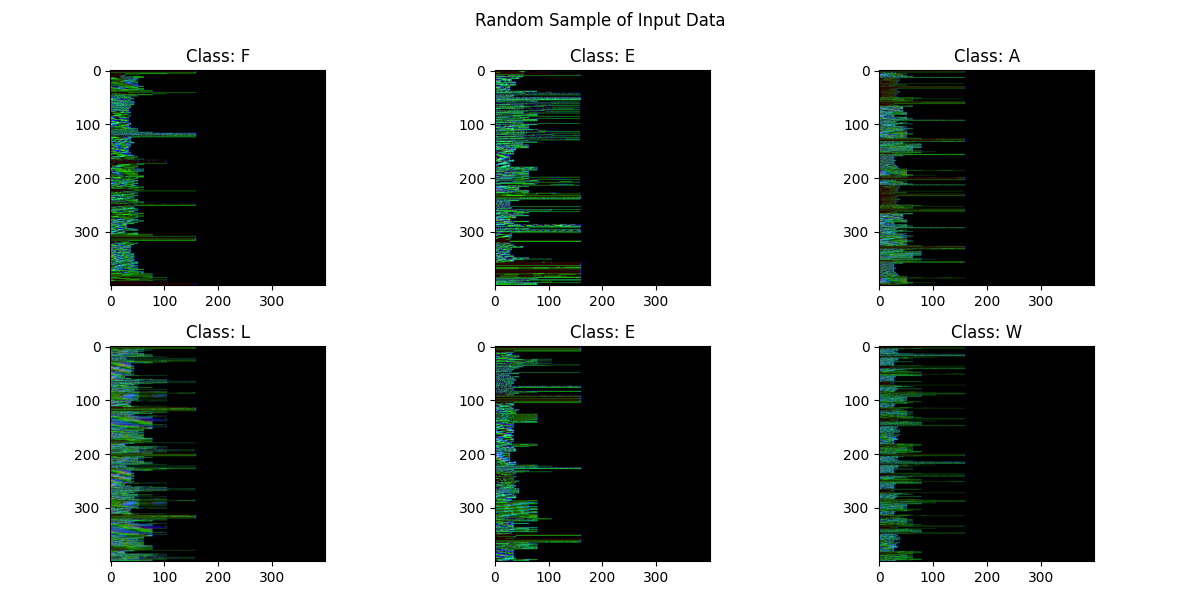
\includegraphics[scale = 0.4]{images_results/CyTex_T1-Initial_Pics/Random Input Sample.png}
        \caption{EMODB - Random CyTex Sample}
        \label{emodb_cytex_imgs}
\end{figure}

\subsection{Pilot Testing and Alterations}
Initially a series of pilot tests were conducted to gauge suitable hyper parameters fro use in the deep learning model. A single simulation was run for varying sets of parameters and the validation accuracy was used to determine the performance of the model. It must be noted that, due to the small size of the EMODB dataset, overtraining is difficult to avoid. By training for a smaller number of epochs with fast convergence, this was marginally mitigated. While pilot tests were conducted on the EMODB dataset, due to the similarity of CyTex images that would be generated for the RAVDESS dataset, the same final hyper parameters were used in that case as well. For each of these trials the EMODB database was randomly split into a train and test set. $80\%$ of the data was grouped into the training set and the remainder into the test set. The random splitting was performed while preserving the balance of classes in both of the data subsets.

\subsubsection{Pilot Test 1:}
For the first pilot test a relatively larger learning rate was employed to allow the model to search rapidly. The ADAM optimization method was used due to its faster convergence than other methods like SGD. It also offers better performance for smaller datasets that can be more prone to noise. A cross entropy loss criterion was also used, which is typical in many image processing tasks. No learning rate scheduler was used as the search habits of this particular learning rate were to be investigated prior to fine tuning. The full list of notable parameters are detailed below.
\begin{itemize}
    \item base model = ResNet50
    \itemsep0em
    \item epochs = 20
    \itemsep0em
    \item mini batch size = 32
    \itemsep0em
    \item $lr = 1e^{-3}$
    \itemsep0em
    \item ADAM weight decay parameter ($\lambda$) = $1e^{-5}$
    \itemsep0em
    \item CyTex overlap = $50\%$
    \itemsep0em
    \item data augmentation (training) = random horizontal flipping and normalization
    \itemsep0em
\end{itemize}
As can be observed in figure \ref{Pilot1_fig}, the convergence for this particular learning rate is far too unstable. That is to say that between epochs the test/validation accuracy is prone to massive fluctuations. This is somewhat unavoidable for smaller non-ideal datasets, however, can be reduced considerably. The best test accuracy achieved in this case was $56\%$. As the training accuracy also seemed to reach a relative ceiling at around $60\%$, it seemed as though the model was having trouble generalizing. By increasing the weight decay parameter ($\lambda$) regularization is also increased. This reduces how large weights can become, in turn reducing model complexity. This parameter was to be modified in future trials.
\begin{figure}[ht]
        \centering
        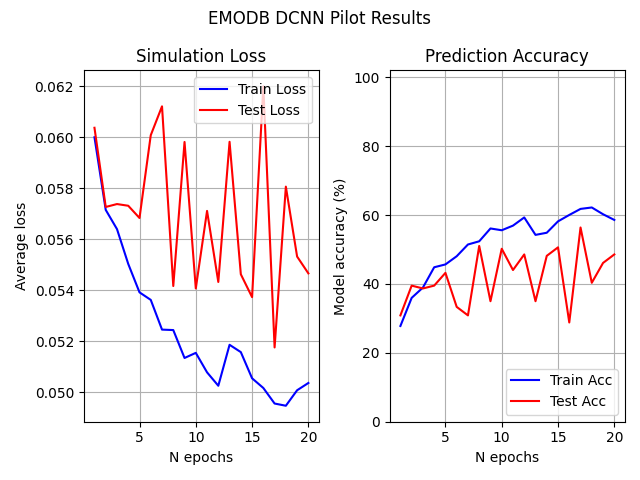
\includegraphics[scale = 0.6]{images_results/EMODB_PilotTests/EMODB_PilotResults_30-05__15-48.png}
        \caption{EMODB - Pilot Test 1}
        \label{Pilot1_fig}
\end{figure}

\subsubsection{Pilot Test 2:}
In the second pilot trial the learning rate was decreased to provide more stable convergence (at the cost of speed). The weight decay was increased to attempt to improve model generalization, reducing large weights present in the model. The number of epochs was also reduced to allow for more rapid pilot testing. While it appears that the model can be trained for longer as the accuracy is still  increasing, this training period is sufficient for parameter comparison and tuning. All parameters not listed below for this trial and future trials can be assumed to be held constant from the previous trial(s). 
\begin{itemize}
    \item epochs = 10
    \itemsep0em
    \item $lr = 1e^{-4}$
    \itemsep0em
    \item $\lambda$ = $1e^{-4}$
    \itemsep0em
\end{itemize}
In this case the convergence was actually faster and more stable. This suggests that the previous learning rate was too large and the model was potentially 'stepping over' local minima and initially missing the ideal solution. The training accuracy was much improved in this trial, informing us that the model is learning more details about the training set. With this more informed model, the test accuracy also slightly improved, reaching a height of $59\%$. It is still apparent that, due to the large difference in training accuracy and test accuracy, the model generalization could be improved. However, the small size of this dataset bring about a fundamental limitation to generalization. 
\begin{figure}[ht]
        \centering
        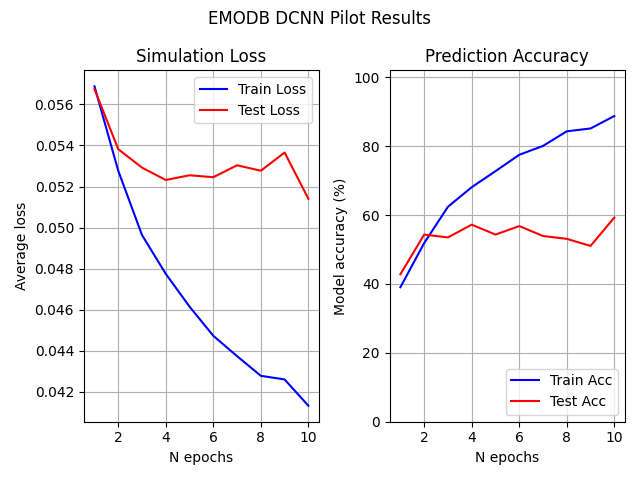
\includegraphics[scale = 0.6]{images_results/EMODB_PilotTests/EMODB_PilotResults_30-05__15-59.png}
        \caption{EMODB - Pilot Test 2}
        \label{Pilot2_fig}
\end{figure}

\subsubsection{Pilot Test 5:}
Pilots 3 and 4 marginally improved accuracy via increasing the learning rate, and hence the search capacity. The number of epochs was also slightly increased. However, due to the minor changes to both parameters and results they are not detailed. Both of these approaches exhibited unstable convergence, as one would expect for a larger learning rate. The fifth pilot test sought to build upon previous trials by attempting to massively improve generalization. The weight decay was increased by a large rate and a number of additional data transformations were applied to the training set, listed subsequently.
\begin{itemize}
    \item epochs = 15
    \itemsep0em
    \item $lr = 1e^{-2}$
    \itemsep0em
    \item $\lambda$ = $1e^{-1}$
    \itemsep0em
    \item data augmentation (training) = random vertical flipping, random rotation, random resized cropping, random horizontal flipping and normalization
    \itemsep0em
\end{itemize}
The results of this test are depicted in figure \ref{Pilot5_fig} and highlight a much more gradual increase in training and test accuracy. A similar scenario was later tested over a larger number of epochs. One may note the much smaller gap between train and test statistics, however, both accuracies are poor. This suggest that the many data augmentation applied, along with increased weight decay, do not allow the model to sufficiently learn the training data. The largest test accuracy obtained over this training interval as $42\%$.
\begin{figure}[ht]
        \centering
        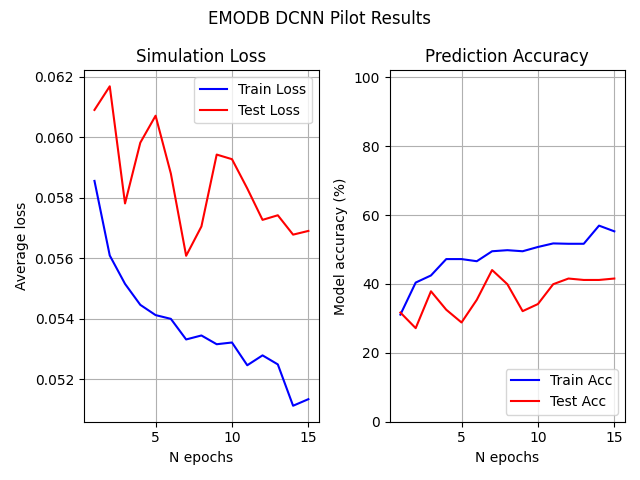
\includegraphics[scale = 0.6]{images_results/EMODB_PilotTests/EMODB_PilotResults_30-05__16-57.png}
        \caption{EMODB - Pilot Test 5}
        \label{Pilot5_fig}
\end{figure}

\subsubsection{Further Pilot Testing:}
A series of further pilot tests were examined in which data augmentation was altered, the number of training epochs was increased to 30 and the learning rate was further modified. However, each of the cases exhibited lower test accuracy than the previous highest result achieved in pilot test 2. Two test which simulated models with lower learning rates over a much longer period (100 epochs) were also tested. However, both of these cases demonstrated poorer accuracy than previous cases. Multi-step scheduling of the learning rate was also applied, however models seemed to be capped at a certain test accuracy which was not sufficient. \\ \\
It was hypothesised that the complexity of the deep learning base model, ResNet50, was too great. A small collection of alternative ResNet models were tested using the exact same experimental conditions and hyper parameters. This collection contained ResNet architectures at depths of 18, 34, and 50 layers. The deeper the model, the higher the complexity. 

% -------------------------------------------
\subsection{K-Fold Cross Validation \& Model Selection}
With the conclusion of the pilot tests a ballpark of optimal parameters were able to be selected. However, parameters were still tuned further during the k-fold testing. 5 folds were used for all instances of cross validation, yielding 80/20 train test splits of the dataset. \textit{Stratified k-fold cross validation} was employed to ensure the preservation of percentages of samples pertaining to each emotion class. The k-fold validation score (test accuracy) was used as the benchmark of model performance as it provides a much better metric for how the model generalizes to other data. It is also necessary for negating 'one off' high achieving results that are not representative of true model performance.\\ \\
The first major round of test conducted altered which ResNet base model was used. For each alteration of base model the following parameters were held constant to allow only the base models to be compared. As mentioned earlier, it was hypothesised that a model with lower complexity and fewer layers may produce greater results due to improved generalization. 
\begin{itemize}
    \item epochs = 10
    \itemsep0em
    \item mini batch size = 32
    \itemsep0em
    \item k folds = 5
    \itemsep0em
    \item $lr = 1e^{-4}$
    \itemsep0em
    \item $\lambda$ = $1e^{-2}$
    \itemsep0em
    \item CyTex overlap = $0\%$
    \itemsep0em
    \item data augmentation (training) = random horizontal flipping and normalization
    \itemsep0em
\end{itemize}
Interpreting the results of each k-fold can be done by examining the vertical yellow lines, which indicate the start of a new fold. At the start of each new fold the model parameters (apart from the first two frozen layers) were reinitialised so that the model could be retrained. Failing to do so would introduce data leakage and corrupt any validity of the results. This is why at each k-fold interval the training and test accuracy dramatically decreases. The results of each fold were plotted in the same figure window to allow for the comparison of results over different folds. For standard presentation one can simply view the results over a single k-fold interval.

\subsubsection{ResNet18 Testing}
First the simplest of the three models was tested, ResNet18. This model was able to be trained in the shortest amount of time and displayed an average test accuracy of \textbf{63.17\%} over the 5 folds. The results of this test are plotted in figure \ref{pilot_r18_fig}. 
\begin{figure}[ht]
        \centering
        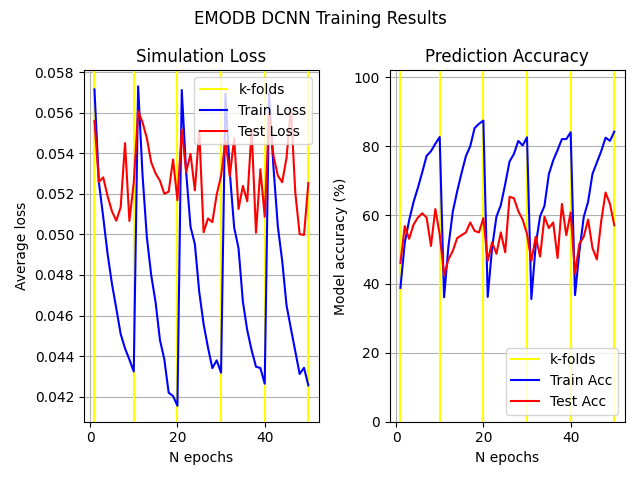
\includegraphics[scale = 0.6]{images_results/EMODB-FinalResults/EMODB_TrainResults_30-05__19-27.png}
        \caption{EMODB - K-Fold Test: ResNet18}
        \label{pilot_r18_fig}
\end{figure}
\subsubsection{ResNet34 Testing}
Next the more complex model, ResNet34 was plotted. This model was considered as a mid-point between the complexity of ResNet50 and the simplicity and potential for lower variance of ResNet18. Results are highlighted in \ref{pilot_r34_fig}, detailing worse performance than ResNet18. The average highest accuracy over each of the 10 epoch folds was \textbf{60.53\%}. While this difference is not dramatic, it definitely points to the fact that greater generalization improves the overall performance of the model for this dataset. 
\begin{figure}[ht]
        \centering
        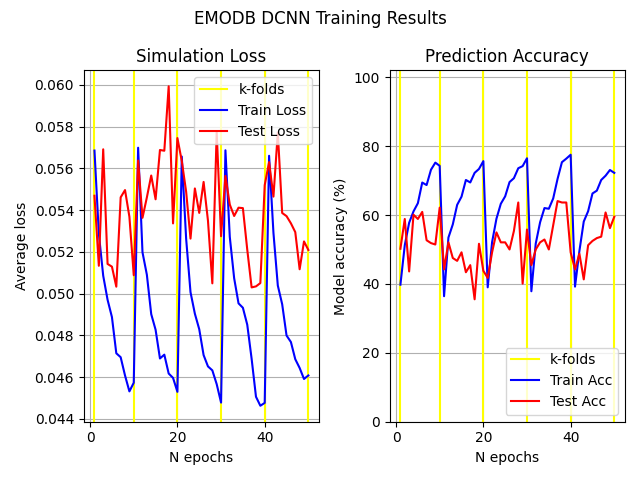
\includegraphics[scale = 0.6]{images_results/EMODB-FinalResults/EMODB_TrainResults_30-05__19-39.png}
        \caption{EMODB - K-Fold Test: ResNet34}
        \label{pilot_r34_fig}
\end{figure}
\subsubsection{ResNet50 Testing}
ResNet50 was then tested using a k-fold cross validation approach. As previous, the model parameters were held constant allowing independent grading of the model. Interestingly, the performance was greater than the ResNet34 model. Although not significantly enough to grade it as a better outright choice. This approach obtained an average highest accuracy of \textbf{61.03\%} over each of the folds. Demonstrating this, one may observe figure \ref{pilot_r50_fig}.
\begin{figure}[ht]
        \centering
        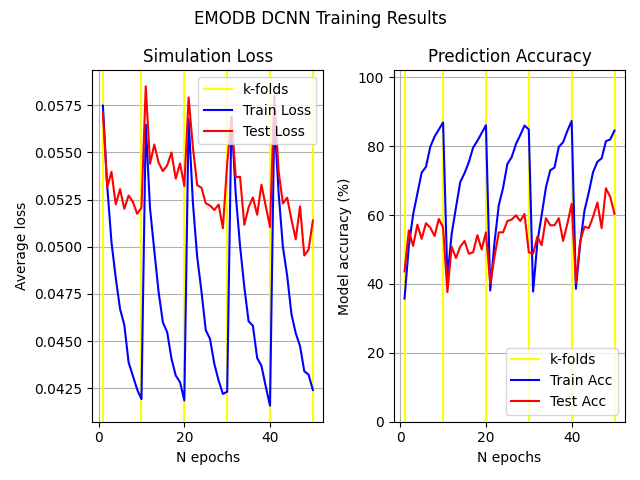
\includegraphics[scale = 0.6]{images_results/EMODB-FinalResults/EMODB_TrainResults_30-05__19-58.png}
        \caption{EMODB - K-Fold Test: ResNet50}
        \label{pilot_r50_fig}
\end{figure}

\subsection{Model Structure and Results}
The final results for the EMODB dataset were attained through use of the ResNet18 model with the additional output layers specified previously in this chapter. Model parameters are listed below. 
\begin{itemize}
    \item base model = ResNet18
    \itemsep0em
    \item epochs = 10
    \itemsep0em
    \item mini batch size = 32
    \itemsep0em
    \item k folds = 5
    \itemsep0em
    \item $lr = 1e^{-4}$
    \itemsep0em
    \item $\lambda$ = $1e^{-5}$
    \itemsep0em
    \item CyTex overlap = $0\%$
    \itemsep0em
    \item no learning rate scheduler implemented
    \itemsep0em
    \item data augmentation (training) = normalization
    \itemsep0em
\end{itemize}
Data augmentation strategies were removed from this approach to create more similar training and test data. This improved the score and while it may lead to overtraining, this should not influence generalization heavily over a small number of epochs. The approach was to reduce model bias rapidly as the pilot testing showed that numerous generalization strategies did not improve the results. A pseudo early stopping criteria was applied in which the parameters of the model with the net highest test accuracy were saved. This preserves a high test accuracy and will minimise the potential for overtraining. The highest accuracy obtained throughout the cross validation process was \textbf{72.7\%} test accuracy. The average test accuracy across each of the folds was \textbf{70.27\%}. The results over each fold are observed in figure \ref{emodb_final_results}.
\begin{figure}[ht]
        \centering
        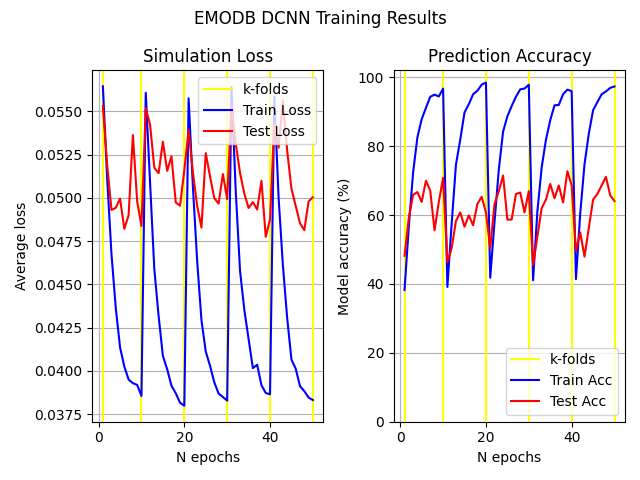
\includegraphics[scale = 0.6]{images_results/EMODB-FinalResults/EMODB_Results_31-05__15-50.png}
        \caption{EMODB - Final Training Results}
        \label{emodb_final_results}
\end{figure}

% SECTION:
% ================================================
\section{RAVDESS Simulations}
This section is significantly shorter than the EMODB results as that database formed the primary set for experimentation and grading model performance. Brief discussions of pilot testing and alterations to the data are included. However, only the final results of the RAVDESS dataset classification are inserted. Other test results can be found on the GitHub repository for this study \cite{Blake_ELEC4840B-Repo}. 

\subsection{Pilot Testing and Alterations}
As mentioned earlier, the results of the EMODB pilot test were largely applicable to the RAVDESS dataset as well. Experiments were conducted, however, roughly the same conclusions were made. The same base model and approximate parameters were identified to give the highest test accuracy. These remained largely unchanged from the previous cases and are detailed in the cross validation  discussion of results on the RAVDESS dataset. The primary difference is the larger number of epochs used due to the greater database size. The RAVDESS dataset took longer to train on in terms of both time and convergence to a solution.

\subsection{Dataset Reduction of Scope}
The RAVDESS dataset possessed more emotions than the EMODB dataset, (8 emotions as compared to 7). As such, the classification was slightly more difficult in this particular case. In attempts to further improve the test accuracy of this method, the number of emotional states for classification was reduced. The reduction of emotional states has been shown to increase a model's prediction accuracy, reducing the number of output classes \cite{zhou2016deep}. In the case of the RAVDESS dataset, the emotions Calm and Surprised exhibit similar characteristics to other emotions present in the dataset. For instance, surprise, prosodically, has features which overlap with fear and happiness given the context of the situation. Calm can also be closely related to a neutral emotion. In terms of the CyTex images generated for both of these emotions, it may be the case that they do not separate themselves enough, saliently, from other emotions in the dataset. Both of these emotions also had no direct equivalent in the EMODB dataset. For these reasons the dataset was truncated to exclude surprised and calm emotional classes for comparison. Results prior to, and after, emotional state truncation are provided in the successive section.

\subsection{Model Structure and Results}
Parameters for RAVDESS simulation were unchanged apart from the duration of simulation and exposure to the training sets. All notable parameters and formats are provided in the ensuing list. A ResNet18 model was once again utilised to reduce complexity of the model. A ResNet50 architecture was also trialled, however, inferior results were obtained.
\begin{itemize}
    \item base model = ResNet18
    \itemsep0em
    \item epochs = 14
    \itemsep0em
    \item mini batch size = 32
    \itemsep0em
    \item k folds = 5
    \itemsep0em
    \item $lr = 1e^{-4}$
    \itemsep0em
    \item $\lambda$ = $1e^{-5}$
    \itemsep0em
    \item CyTex overlap = $0\%$
    \itemsep0em
    \item no learning rate scheduler implemented
    \itemsep0em
    \item data augmentation (training) = normalization
    \itemsep0em
\end{itemize}
For the entire RAVDESS dataset an average test accuracy, across 5 folds, of \textbf{50.72\%} was recorded. As expected, reducing the number of output classes yielded a higher average test accuracy of \textbf{56.87\%}. These metrics relate to the results presented in figures \ref{ravdess_final_results} and \ref{ravdess_trunc_results}, respectively. The differences in accuracy between this dataset and the EMODB dataset are discussed in the following section. While these results are not as favourable as previous recordings, they do not form the primary judgement over the models performance. Further, the original CyTex study did not include exploration of this dataset, so the comparison to CyTex's previous performances cannot be made. One point of interest is that the initial accuracy of each fold is considerably lower than that of figure \ref{emodb_final_results}. This suggests that the base model and initial weights have more trouble describing and classifying the data in this set. In future trials, a slower converging extended epoch simulation should be conducted. This method would more intimately explore the characteristics and could benefit from the increased size of the RAVDESS dataset. While approaches similar to this were attempted, no promising results were gathered.
\begin{figure}[ht]
        \centering
        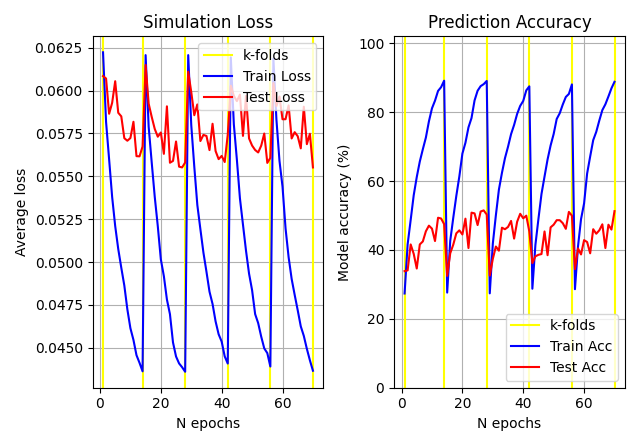
\includegraphics[scale = 0.6]{images_results/RAVDESS-FinalResults/RAVDESS_Results_31-05__19-18.png}
        \caption{RAVDESS - Final Training Results}
        \label{ravdess_final_results}
\end{figure}
\begin{figure}[ht]
        \centering
        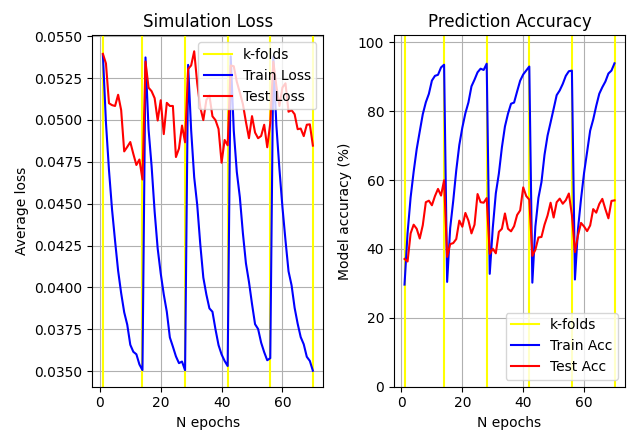
\includegraphics[scale = 0.6]{images_results/RAVDESS-FinalResults/RAVDESS_Results_01-06__12-17.png}
        \caption{RAVDESS - Truncated Data Results}
        \label{ravdess_trunc_results}
\end{figure}

% SECTION:
% ================================================
% PROBABLY NOT NECESSARY
% \section{Advanced Simulations}
% \textbf{*** Only add this section if given extension to alter CyTex images and further improve results. Also could include MEL Spectrogram results here.}


% SECTION:
% ================================================
\section{Discussion of Results}
This section discusses the results obtained for the two datasets considered in this study. The result achieved for the EMODB case is of a relatively high standard and is compared to validation/test results obtained by Zhao et al. \cite{ZHAO2019}. A discussion of the experimental design for achieving these results is covered. This includes information on how these results should be interpreted and whether or not they are directly comparable to other benchmark methods (including the foundational CyTex paper on which this work is based).  Concluding this section, suggestions for future experiments are put fourth with hopes of improving these results in further trials. The key results which will be referenced throughout this section pertain to table \ref{CytexResults_table}.
\begin{table}[ht]
    \centering
    \begin{tabular}{|l|c|c|}
    \hline
    Database & \multicolumn{1}{l|}{Highest Test Accuracy} & \multicolumn{1}{l|}{Average Fold Test Accuracy} \\ \hline
    \textbf{EMODB}             & 72.7\%  & 70.27\% \\ \hline
    \textbf{RAVDESS}           & 51.48\% & 50.72\% \\ \hline
    \textbf{Truncated RAVDESS} & 59.94\% & 56.87\% \\ \hline
    \end{tabular}
    \caption{Summary of CyTex Results}
    \label{CytexResults_table}
\end{table}

\subsection{Interpreting \& Comparing Results}
The main metrics used to gauge the performance of a model on a particular dataset in this report is the average test accuracy over five folds. This metric is often used in SER  literature due to the small  size of many widely used datasets. Another common measure is the average accuracy found over each of the emotional classes. This measure was not used at it does not accurately enough imply how a model may generalize. However, it does provide greater insight into particular classes or features that the model may have trouble classifying. In future this metric should also be included for a greater breadth of comparison.\\ \\
When comparing these results to contemporary benchmarks, we must first find suitable points of comparison. For the results on the EMODB dataset, the highest accuracy achieved rivals the validation accuracy observed in figure \ref{zhao2019_train_fig} \cite{ZHAO2019}. As this is considered a state  of the art method, our models achieves a good result in the training and validation phase. However, the average accuracies recorded over classes is likely significantly higher than this study of the CyTex methodology.\\ \\
The original results of Bakhshi et al. using the CyTex transform may be noted as significantly more accurate \cite{CyTexRef}. However, it is important to note the differences in experimental approach. A much more complicated base model of ResNet152 was utilised for their approach. More advanced computing resources were also available, which can have a direct impact on the accuracy of an assessed system. It is also likely that the quality and structure of CyTex images generated are noticeably different. The exact same process of image generation was not used, so it is likely that the parameters used in this study's approach are not as optimal as those used in the foundational study. This is also evidenced by the large gap between training and test accuracy in all figures detailing the training results of this thesis. A large training accuracy highlights the fact that the model is successful at identifying patterns in the training data. No difficulties exist that prevent the model from adequately learning. This points to the source of mismatch in accuracy metrics resulting from the CyTex images themselves. Despite the model learning, the images are not expressive or salient enough to yield more impressive results on validation sets. Potential improvements to the underlying CyTex images are discussed later.\\ \\
As far as the results evaluated on the RAVDESS dataset, significantly more work need be done to produce a noteworthy result. The TIM-Net model, currently holding one of the highest performance metrics for this dataset, is dramatically more accurate that the method detailed in this paper. TIM-Net achieves a UAR score of $91.93\%$ on this dataset \cite{ye2023temporal}. This approach employs 10-fold cross validation, and while it is not directly analogous to the metrics of table \ref{CytexResults_table}, it clearly details a need to improve this strategy's results.


\subsection{Improving Results in Further Experiments}
A number of strategies for improving the results are provided below. It is predicted that the greatest positive improvement of results would be seen by modification of the generated CyTex images used for training and evaluation. Methods for improving the validity and comparability of results are also discussed.
\subsubsection{CyTex Parameter Tuning}
As was noted, it is likely that the generated CyTex images are the source of less than optimal accuracy in each of the test settings. By further tuning parameters used to generate these images the quality of the transform should increase. It is important to note that these parameters may need to be tuned on a per dataset basis.\\ \\
The maximum frequency threshold ($\mathbf{f_{max}}$) able to be extracted by the librosa piptrack method should be stepped by intervals of $100Hz$. For experiments conducted in this work, a maximum of $400Hz$ was used as this should include the standard operating frequency of human speech. However, two potential scenarios could be affecting the resultant images. The first scenario is that the maximum threshold is too large and too much frequency data is included. This means that information that is not useful for the classification of emotional speech is making its way into the CyTex images. The other case is that the maximum threshold is too low and there exists data samples which exhibit frequencies larger than the maximum threshold. If this is the case, the piptrack method may be truncating important information that could inform the basis of classification.\\ \\
Framing can produce differing results as well. While $10ms$ is a common choice, this value may not be optimal for the RAVDESS dataset. Some literature uses values somewhat larger than this interval, which could change the performance of a model. Values significantly larger should not be used, however. This would result in speech frames that are no longer able to be considered stationary and the granularity of fundamental frequencies extracted would be too coarse. Varying this frame length between $10ms$ and $40ms$ may produce some difference to the observed results, particularly for the RAVDESS database. It has been found, experimentally, that $10ms$ is a suitable measure for the EMODB database experiments.\\ \\
Finally, the additional dimensions of encoding the RGB images could be substituted for different kinds of information. Horizontal and vertical gradients were used in this application, but this information may not be optimal. A wealth of other encoding schemes could be used, including previously discussed strategies like Laplace Transform information.

\subsubsection{MEL Spectrogram Comparison}
In order to better determine whether the model needs improvement and to give a better baseline for model performance, MEL-Spectrograms should be generated for each of the samples in a given dataset. The model can then be trained and evaluated on this set of image data. We expect the performance of a properly employed CyTex method to be greater than that of a MEL spectrogram approach. If this is not the case, we can infer that our CyTex images need be further improved to better represent the dataset. If the MEL-Spectrogram trained model also performs poorly, it is inferred that the model is a poor candidate for exhibiting exemplary results.

\subsubsection{Alternate Performance Metrics}
During this thesis, only training and validation sets were used. This is why the terms test and validation have been used interchangeably in places. The decision to do so was to recreate the experimental conditions from the original CyTex study conducted by Bakhshi et al. The small size of a dataset like the EMODB also necessitates this as splitting this set into 3 subsets (training and independent test and validation sets) can compromise the validity of results. In this case, either the test and validation sets will be too small to gain meaningful information about generalization. Or, the training set will be too small to sufficiently learn the model. That being said, in future the use of independent test and validation sets would help obtain results that are more closely comparable to other studies in the literature.

\subsubsection{Data Augmentation Injection}
Thanapol et al. suggest improved generalization using a novel approach to data augmentation \cite{Thanapol2020}. In this study, CNN models are initially trained on non-augmented data samples, similarly to the approach taken in this thesis. This encourages an initial fast convergence to a solution. However, after 30 epochs the training data is inject with data augmentations. This means that after a model has learned the more basic features to broadly classify input data, it then gains a better capacity to generalise, minimising overfitting. An approach like this would be interesting to study and may improve performance metrics.




% ===========================================
%	Chapter 6
% ===========================================
% \chapter{Extending CyTex to Alternate Data Sources}\label{ch-ext-cytex}
The CyTex transform has previously demonstrated tremendous results on a number of benchmark datasets within the SER domain \cite{CyTexRef}. However, what is currently unknown, is the performance of such a method in alternate classification domains. This transformation method would prove even more powerful should its applications expand into these other types of problems. For this reason, this study also seeks to attempt to successfully extend the CyTex transforms use cases into additional domains. This section details the underlying theory and experimental results of such alternate data extensions. I should be noted that the extensions explored are not comprehensive and the CyTex transform may have further applications not explored in this project.\\ \\
\textbf{***USE THIS RESOURCE \cite{won2021music}!}


% =================================================
\section{Alternate Audio Data Sources}


% =================================================
\section{Classifying Musical Instruments OR NOTES}
\subsection{Musical Instrument Signals}


\subsection{Monophonic and Polyphonic Signals}


% =================================================
\section{Benchmark Musical Databases and Methods}


% =================================================
\section{CyTex in a Musical Context}
\subsection{CyTex Suitability}
As musical instruments produce acoustic signals, which typically exist within the human range of hearing, they are naturally similar to speech signals produced by humans. For this reason it is hypothesised that some meaningful patterns should be identifiable by a CyTex transformed deep learning process. 

\subsection{CyTex Classification Results}




% ===========================================
%	Chapter ***[REDUNDANT]***
% ===========================================
% section altered and removed for PART B
% \chapter{Planning for Future Research - ELEC4840B}\label{ch-plan}
Having completed the interim portion of this project requires planning for the following phase of this honours thesis. This section proposes milestones and work scheduling required to achieve the established deliverables of this project. Also outlined are brief descriptions of active areas of interest pertaining to the CyTex transformation. These areas aim to be explored in the remainder of the thesis. Such areas include further review of contemporary literature, better articulating the methods CyTex employs, and extending the CyTex transform in novel ways.


% -----------------------------------
\section{Project Milestones}
\begin{description}
\item[Deep learning model construction:]
Using a transfer learning approach, a suitable DCNN will be constructed. This model will be closely aligned with the fine-tuned ResNet152 DCNN model utilised in \cite{CyTexRef}. Following the creation of the model the training period will commence. The expectation is that this process may take some time (potentially over a week per dataset). For this reason some of the subsequent milestones will be completed in parallel with this task.

\item[Recreation of CyTex results:]
After the development and training of a DCNN for EMODB and additional databases, the validation phase will begin. An accuracy approxiamte to those seen in \cite{CyTexRef}
% , \textbf{*** Ref table if inserted into my report!},
should be demonstrated. Having done so gives a baseline for the implementation of the method. Demonstrating correct implementation and adaptation to the relevant datasets. The primary goals of the thesis, to this point, have been rooted in gaining knowledge in the subject area and proving understanding via successful execution of learnt concepts. Beyond this point the dissertation will delve into new territory. The subsequent milestones investigate areas that have not necessarily been explored before, at least in terms of the CyTex transform. 

\item[Alternative $F_0$ representations:]
The basis of the CyTex transform relies heavily on the calculation of the fundamental frequency of specified length audio frames. By combining the frequency information over a larger time frame one can essentially replicate a multi-resolution analysis technique. Currently, key frequency information is calculated through use of the librosa package \cite{mcfee2015librosa}. This particular package employs an STFT using methods highlighted in \cite{SASPWEB2011_stanford}. However, there are a number of alternate methods available, producing a similar function. Further literature review into each of these methods will be conducted. Following this, the implementation of suitable candidate methods will be tested and compared to the baseline method. Upon comparison of alternate time and frequency analysis practices, recommendations will be made to ensure CyTex performance is maximised. Among the time and frequency analysis strategies investigated will be,
\begin{itemize}
    \item The Fourier Transform.
    \item The Short-Time Fourier Transform.
    \item The Gabor Transform.
    \item The Wavelet Transform.
\end{itemize}

\item[Generalising CyTex to other data sources:]
After execution of CyTex and investigation of improved fundamental frequency calculation, the transform's operation will be applied to other data sources. Areas of interest include classification of musical instruments, identification of artificially simulated sound sources, and animal classification. However, this investigation will largely depend on the accessibility of high quality, labelled, open-source data. For a number of the previously mentioned data types this may pose an issue.

\item[Identifying weaknesses of CyTex:]
Upon generalising CyTex and testing the transforms accuracy over various scenarios, the potential weaknesses of the transform should become evident. Should this not be the case, further testing and review of literature will be conducted to recognize such deficiencies. This identification is necessary for future researchers to be weary of ahead of their interactions with the transform. A set of scenarios for which CyTex is a prime candidate of feature extraction may be developed. It may also spawn an active interest in fortifying CyTex and removing such vulnerabilities for more consistent results. The flaws highlighted will also shape the direction of the investigation into extensions applied to CyTex in both this paper and future papers.

\item[Investigation of CyTex extensions:]
The final proposed milestone of the thesis involves investigating contemporary methods and proposing novel advancements to CyTex. It should be noted that this milestone is time dependent and the level of completion is not guaranteed, nor the final outcome. At the very least, however, the thesis will aim to suggest exciting topics for future research. As well as key areas for the CyTex transform to gain further relevance within the expanding field of SER. A number of potential enhancements are detailed in the following section of this report. It is likely that, due to time constraints and limiting of the project scope, only a single innovation (at most) will be thoroughly researched and employed.

\end{description}


% -----------------------------------




% ===========================================
%	Chapter 7
% ===========================================
\chapter{Concluding Remarks}\label{ch-concl}
In studying and evaluating the CyTex transform as a means of emotional classification from speech, this chapter summarizes and expands upon some of the key findings of this report. As a number of the strengths of this method have been discussed in previous chapters, these are not addressed here in great detail. Instead, focus is dedicated towards identifying the weaknesses of this method and improving/extending this method for future research. A small list of tasks which will be undertaken to prepare for project demonstration is also discussed.

% \section{Strengths of the CyTex Image}
% Lossless transform\\
% Higher accuracy than other methods\\
% Allows for simple deep learning application and rapid + efficient training\\


\section{Weaknesses of the CyTex Image}
The CyTex transform has the benefit of only requiring knowledge of the fundamental frequency. While this means that the transform can be executed with limited information and processing, it also has its drawbacks. Depending heavily on a single characteristic of input data means that the CyTex transforms quality is entirely dependent on the method of extraction of that particular characteristic. In the case of this application, the piptrack method from the librosa library influences all results obtained \cite{mcfee2015librosa}. While this library is commonly used, alternative approaches should be investigated. Additionally, the other channels of the RGB image are also related to the fundamental frequency. These channels could instead be encoded with information relating to other prosodic features of the audio data.\\ \\
For extending CyTex to other acoustic domains, it is likely that significant reworking is required to generalise this transform. One may consider an extension to the domain of musical instrument classification. Musical instruments operate over a larger bandwidth than that of the human range of speaking. Furthermore, different instruments may also produce spectra of noise that significantly overlaps with that produced by other instruments. We can then infer that pitch will not be an ideal determining factor for classification.\\ \\
Evaluations on the RAVDESS dataset suggest that optimal tuning of CyTex parameters may be dataset dependent. This is particularly relevant for extending CyTex beyond the realms of human emotional speech data. The frequency range must be researched for each application such that relevant information is not lost during pitch extraction.\\ \\
While the utilisation of CyTex images, although not compared in this study, has been demonstrated to be superior to MEL-Spectrograms, they require more work to implement. Packages and libraries exist for the generation of MEL-Spectrogram images and, due to the infancy of CyTex, the same community support does not exist.


\section{Enhancements for Project Demonstration}
Prior to the demonstration of the project, the following advancements are planned to be introduced to this project. Each point seeks to improve the results in terms of accuracy, validity and applicability, respectively.
\begin{description}
\item[Additional tuning of CyTex parameters:]
In attempts to improve the accuracy of the methods discussed in this paper, the parameters of the CyTex image generative script will be progressively tuned. Following each tuning the proposed DCNN model will be trained and evaluated to see if the average test accuracy is increased. The primary parameter to be tuned is the maximum frequency threshold, however, the frame lengths and channel encoding may also be investigated. 

\item[Introduction of separate test set:]
Results will be recreated using a different composition of data for training and validating. However, the introduction of an independent test set which is separate from both the training and validation sets will be used. The proposed data split still utilises $80\%$ of the total data as the training set. However, the remaining data will be evenly divided into validation and test sets. The validation set will be used as a grade of performance during training. The test set will act as unseen data by the model and will be used to generate confusion matrix plots. This output will specify the accuracy displayed for each emotional class and also give information on which classes the model finds more difficult to categorise. 

\item[Development of an interactive presentation:]
A script will be developed which takes, as input, a user recorded speech sample. This speech sample will then be converted into a group of CyTex images (depending on the length of the signal) and analysed using the highest performing model trained on an English speaking dataset (RAVDESS). A barplot will be produced as the output, detailing the percentage of each emotion displayed by the user, aggregated over each of the generated CyTex images. It is acknowledged that the accuracy of such tests will be poor due to the significant difference between user simulated data and the training set. However, this extension merely seeks to provide a novel and interactive means of applying the technology presented in this work.

\end{description}

\section{Areas for Innovation}
\begin{description}
\item[Extending CyTex to higher dimensions:]
One of the major benefits of the CyTex transform is the ability to encode additional feature information by transforming an audio signal into a two-dimensional textured image. This can potentially be taken a step further, however. By training the machine learning model with more information dense inputs, one would expect that the output classification would improve in accuracy. Additional information can be encoded into the input via creating inputs of larger dimensions. For example, a speech to three-dimensional image/object transform could be constructed. This extra dimension could encode information that would aid the classification of emotion. A third dimension could also be used to give greater temporal information, similar to the approach taken by Kim et al. \cite{kim2017speech}.

\item[Generalise CyTex to other forms of acoustic data:]
As of this time, CyTex has only been utilised in conjunction with human speech data. It is of great interest to substitute this training data for alternate data sources. In doing so, the applications for CyTex may become incredibly broad. One of the largest areas of interest in this region is that of animal data. Candidate datasets for such purposes have been identified. Particular datasets that appear promising for this task include the BirdVox-DCASE-20k and ESC-50 datasets, \cite{lostanlen_vincent_2018_1208080}, \cite{piczak2015dataset}. The BirdVox-DCASE-20k dataset is segmented in 10 second clips, which is an appropriate format for CyTex analysis. Both datasets also contain many samples, however, the ESC-50 contains audio types other than animals. Some additional sorting of the ESC-50 dataset must be performed prior to any kind of analysis. It is also hypothesised that pitch would yield sufficient identifiable characteristics to be able to differentiate between different animals. This means that the CyTex transform need not be significantly modified to sufficiently represent animal data. 
\\ \\
Another interesting domain for the application of CyTex is the musical audio domain. The most directly relevant classification problem is the classification of the emotion of music, however, this has not been investigated in any great depth. Musical instrument classification in monophonic and polyphonic audio samples can also be approached. However, as previously noted, significant restructuring of the CyTex transform need be applied. The IRMAS dataset has been identified as a suitable candidate dataset for such applications \cite{bosch2012comparison}.
\end{description}


\section{Conclusion}
A successful review and inflation of literature pertinent to the CyTex transform was conducted. This thesis serves as a reference for those seeking to engage with CyTex and relevant SER literature. Many of the foundational concepts required for image classification in the SER domain were collated and surveyed within this body of work. In reading this report, one also gains sufficient knowledge of existing challenges faced by the SER domain and the CyTex transform specifically.\\
CyTex images were generated for different datasets and interpreted by deep learning models using a transfer learning approach. This made use of one of the key advantages of the lossless speech to image transform, in utilising a pre-trained state of the art model.\\
Key performance metrics were adequate in the instance of the EMODB dataset and were comparable with a select group of established methods. However, further adjustments to the structure and composition of the CyTex images should yield a classification accuracy closer to the results achieved by the original implementation of this transform. Additional tuning of the deep learning model should also be employed to improve the results demonstrated on other datasets.





% ===========================================
\singlespacing

\bibliographystyle{apalike}  
% or: plain,unsrt,alpha,abbrv,acm,apalike,...
\bibliography{22S2FYP}
\clearpage



\appendix
% APPENDIX: ReadMe, Copyright permissions
% 
% 
% \pagenumbering{roman}  % make sure that front matter is numbered roman
%\renewcommand*{\thepage}{A\roman{page}}

\chapter{Readme File}\label{Apndx:readme-ga-eoc}
\makeatletter 
\renewcommand{\thefigure}{S\@arabic\c@figure}
\renewcommand{\thetable}{S\@arabic\c@table}
\makeatother


\section*{How to Use the Software}



\chapter{Permissions for Copyrighted Materials}\label{Apndx:license}
This chapter in the appendix includes the first page of each acquired licenses of the figures and excerpt of papers used in the thesis. %I obtained licenses to the inclusion of figure for both in the printed and online version of the thesis from respective copyright holder.



% Glossary:
%           Alpahbetised 
% 
%\backmatter

\chapter{Glossary} % \addcontentsline{toc}{chapter}{List of Symbols}

    % Template:
    % $$ & {} \\
    
	\begin{longtable}{ll}
    % 0. Abstract
    
	
	% 1. Introduction
    $SER$ & {Speech Emotion Recognition} \\
    
    
    % Speech Signal Intro
    $F_0$ & {Fundamental Frequency} \\

    % 1.5 Basics of Acoustics
    $DSP$ & {Digital Speech Processing} \\
    $T_0$ & {Sampling Period} \\
    $f_0$ & {Sampling Frequency} \\
    $DTFT$ & {Discrete-Time Fourier Transform} \\
    $LPF$ & {Low Pass Filter} \\
    $LTI$ & {Linear Time Invariant} \\
    $DFT$ & {Discrete Fourier Transform} \\
    $STFT$ & {Short-Time Fourier Transform} \\
    $Stationary$ & {Non-varying with respect to time} \\
    
    % 3. Lit Review
    $LSTM$ & {Long Short Term Memory} \\
    $LFLBs$ & {local feature learning blocks} \\
    $ MTL$ & {Multi-Task Learning} \\
    $TIM-Net$ & {Temporal-aware bI-direction Multi-scale Network} \\
    $MFCCs$ & {Mel-Frequency Cepstral Coefficients}  \\
    $UAR$ & {Unweighted Average Recall} \\
    $WAR$ & {Weighted Average Recall} \\
    $SAE$ & {Stacked Autoencoder} \\
    $DBN$ & {Deep Belief Network} \\
    $RBM$ & {Restricted Boltzmann Machine} \\
    
    % 4. Theory
    $SUSAS$ & {Speech Under Simulated and Actual Stress} \\
    $EMODB$ & {Emotional Database of Berlin} \\
    $RAVDESS$ & {Ryerson Audio-Visual Database of Emotional Speech and Song} \\
    $IEMOCAP$ & {Interactive Emotional Dyadic Motion Capture} \\
    $DCNN$ & {Deep Convolutional Neural Network} \\
    $Stationary$ & Non-changing frequency and spectral contents over time \\
    $AI$ & {Artificial Intelligence} \\
    $i.i.d.$ & {independent and identically distributed} \\
    $CNN$ & {Convolutional Neural Network} \\
    
    % 4. Future Research
    
    
	\end{longtable}



%\printindex

\end{document}